\documentclass{skripsimathugm}
\graphicspath{{figures/}{figures/Gambar FHO/}{attachments/}}

%-----------------------------------------------------------------
%Disini awal masukan untuk data Skripsi (ISI SESUAI DENGAN DATA ANDA!)
%-----------------------------------------------------------------
\titleind{
OPTIMALISASI SISTEM \textit{ELECTRIC BIKE-SHARING} DI YOGYAKARTA DENGAN PENDEKATAN OPTIMISASI STOKASTIK DUA TAHAP MENGGUNAKAN \textit{FIRE HAWK OPTIMIZER}
}

\titleeng{
ELECTRIC BIKE-SHARING SYSTEM OPTIMIZATION IN YOGYAKARTA WITH TWO-STAGE STOCHASTIC OPTIMIZATION APPROACH USING FIRE HAWK OPTIMIZER}

\fullname{Saddam Aditya Hartanto}
\NIM{20/459353/PA/20014}
\yearenrollment{2020}
\examdate{17 Oktober 2024}
\degree{Sarjana Matematika}
\yearsubmit{2024}
\firstsupervisor{Dr. Noorma Yulia Megawati, M.Sc.}
\firstexaminer{Dr. Fajar Adi Kusumo, S.Si., M.Si.}
\secondexaminer{Dr. Indarsih, S.Si., M.Si.}
\thirdexaminer{Dr.rer.nat. Yeni Susanti, S.Si., M.Si.}



\begin{document}

\cover\titlepage
\approvalpage
\declarepage
%Setelah Anda selesai Ujian Akhir Skripsi, scan halaman pengesahan yang telah ditandatangani dosen pembimbing dan penguji, scan juga halaman pernyataan yang telah Anda tandatangani. Selanjutnya simpan hasil scan tersebut dalam bentuk PDF dengan nama pengesahanskripsi.pdf dan pernyataan.pdf (file disimpan di folder yang sama dengan folder dimana file Skripsi.tex tersimpan)
%Hilangkan karakter % sebelum perintah "\approvalpagescan" dan "\declarepage" di bawah ini, dan tambahkan karakter % sebelum perintah "\approvalpage" di atas.
%\approvalpagescan
%\declarepagescan

%-----------------------------------------------------------------
%Halaman Persembahan (ISI SESUAI DENGAN DATA ANDA!)
%-----------------------------------------------------------------

\acknowledment
\begin{flushright}
\Large\emph\cal{Untuk penulis di masa lalu\\
yang telah berjuang dengan segala keterbatasan,\\
tidak menyerah meski dalam kesulitan.}
\end{flushright}
%-----------------------------------------------------------------
%-----------------------------------------------------------------


%-----------------------------------------------------------------
%Halaman Motto (ISI SESUAI DENGAN DATA ANDA!)
%-----------------------------------------------------------------
\motto
\emph{"\textit{Try to find the argmax over the things that you're interested in}"}
\begin{flushright}
(Andrej Karpathy)
\end{flushright}
%-----------------------------------------------------------------
%-----------------------------------------------------------------


%-----------------------------------------------------------------
%Disini awal masukan untuk Prakata (ISI SESUAI DENGAN DATA ANDA!)
%-----------------------------------------------------------------
\preface
Puji dan syukur Penulis panjatkan ke hadirat Allah Subhanahu Wa Ta’ala, karena atas rahmat dan karunia-Nya Penulis bisa menyelesaikan Skripsi yang berjudul ”Optimalisasi Sistem \textit{Electric Bike-Sharing} dengan Pendekatan Optimisasi Stokastik Dua Tahap Menggunakan \textit{Fire Hawk Optimizer}”. Shalawat serta salam Penulis curahkan kepada Nabi Muhammad Shalallahu’Alaihi Wassalam dan semoga kita mendapatkan syafaatnya kelak.

Penulisan Skripsi ini bertujuan untuk memenuhi salah satu syarat memperoleh gelar sarjana Program Studi S1 Matematika Fakultas Matematika dan Ilmu Pengetahuan Alam Universitas Gadjah Mada. Dalam penulisan dan penyusunan Skripsi ini tentunya tidak terlepas dari bantuan, bimbingan dan dukungan dari berbagai pihak. Oleh karena itu, Penulis ingin menyampaikan ucapan terima kasih
kepada :

\begin{enumerate}
    \item Prof. Dr. Eng. Kuwat Triyana, M.Si. selaku Dekan Fakultas Matematika dan Ilmu Pengetahuan Alam, Universitas Gadjah Mada
    \item Dr. Nanang Susyanto, S.Si., M.Sc. selaku Ketua Departemen Matematika Fakultas Matematika dan Ilmu Pengetahuan Alam, Universitas Gadjah Mada.
    \item Dr. Sutopo, S.Si., M.Si. selaku Ketua Program Sarjana Program Studi Matematika, Fakultas Matematika dan Ilmu Pengetahuan Alam, Universitas Gadjah Mada.
    \item Dr. Noorma Yulia M., S.Si., M.Sc. selaku dosen pembimbing tugas akhir yang telah membimbing penulis, memberikan ilmu, semangat, dan motivasi sehingga penulis dapat menyelesaikan skripsi ini.
    \item Prof. Dr.rer.nat. Indah Emilia Wijayanti, M.Si. selaku dosen pembimbing akademik penulis selama menimba ilmu di Program Studi Matematika, Universitas Gadjah Mada.
    \item Seluruh civitas akademika Fakultas Matematika dan Ilmu Pengetahuan Alam, Universitas Gadjah Mada khususnya seluruh dosen yang telah sabar membagikan ilmunya kepada Penulis.
    \item Ayah dan Ibu yang selalu memberikan dukungan moral dan motivasi kepada penulis untuk selalu melangkah ke depan, serta Adik tercinta Iqbal Prakusa Hartanto.
    \item Amelia Gina Salsabila beserta keluarga yang turut memberikan dukungan maupun saran dalam penyusunan Tugas Akhir.
    \item Dosen pendamping, PI-Koor, serta seluruh panitia LMNas 34 dan Semnastika 15 terkhusus Fauzan Nauvally Muhammad yang telah banyak membantu kesuksesan LMNas 34 dan Semnastika 15.
    \item Madellin de Cartelle dan teman-teman Kondik yang sering menampung keluh kesah kuliah.
    \item Tim \textit{Wastewater Surveillance} yang turut mendukung segera selesainya penulisan Tugas Akhir.
    \item Teman-teman mahasiswa Program Studi S1 Matematika Angkatan 2020, kakak dan adik tingkat yang membersamai dan membantu Penulis baik dalam menjalani perkuliahan maupun dalam penyusunan Skripsi ini.
    \item Seluruh pihak yang terlibat dalam proses penyelesaian Skripsi ini yang tidak dapat disebutkan satu per satu.
\end{enumerate}

\vspace{0.8cm}

\begin{tabular}{p{7cm}c}
&Yogyakarta, 17 Oktober 2024\\
&\\
&\\
&Penulis
\end{tabular}
%-----------------------------------------------------------------
%-----------------------------------------------------------------
%-----------------------------------------------------------------
%Daftar Isi (TIDAK PERLU DIUBAH)
%-----------------------------------------------------------------
\newpage\phantomsection\addcontentsline{toc}{chapter}{DAFTAR ISI}
\makeatletter\renewcommand\l@chapter[2]{\ifnum \c@tocdepth >\z@\addpenalty\@secpenalty\addvspace{0em}\setlength\@tempdima{2.5em}\begingroup\parindent \z@ \rightskip \@pnumwidth\parfillskip -\@pnumwidth\leavevmode \bfseries\advance\leftskip\@tempdima\hskip -\leftskip#1\nobreak\ \leaders\hbox{$\m@th\mkern \@dotsep mu\hbox{.}\mkern \@dotsep mu$}\hfil\nobreak\hb@xt@\@pnumwidth{\hss #2}\par\endgroup\fi}\makeatother
\begin{singlespacing}\tableofcontents\end{singlespacing}
%-----------------------------------------------------------------
%-----------------------------------------------------------------

%-----------------------------------------------------------------
%Daftar Tabel (JIKA DIPERLUKAN, HAPUS KARAKTER % SEBELUM \newpage dan \begin)
%-----------------------------------------------------------------
\newpage\phantomsection\addcontentsline{toc}{chapter}{DAFTAR TABEL}
\begin{singlespacing}\listoftables\end{singlespacing}
%-----------------------------------------------------------------
%-----------------------------------------------------------------

%-----------------------------------------------------------------
%Daftar Gambar (JIKA DIPERLUKAN, HAPUS KARAKTER % SEBELUM \newpage dan \begin)
%-----------------------------------------------------------------
\newpage\phantomsection\addcontentsline{toc}{chapter}{DAFTAR GAMBAR}
\begin{singlespacing}\listoffigures\end{singlespacing}
%-----------------------------------------------------------------
%-----------------------------------------------------------------


%-----------------------------------------------------------------
%Daftar Lambang (ISI SESUAI DENGAN DATA ANDA!)
%-----------------------------------------------------------------
\lambang
\begin{tabular}{ccp{10.5cm}}
$\Omega$ &:&  Himpunan skenario\\
$K_\omega$ &:&  Himpunan perjalanan dalam skenario $\omega$\\
$S$ &:&  Himpunan lokasi potensial stasiun\\
$T$ &:&  Himpunan periode waktu\\
$H$ &:&  Himpunan sepeda\\
$\pi_\omega$ &:&  Probabilitas skenario $\omega$\\
$p_k$ &:&  Kontribusi keuntungan perjalanan $k$\\
$F_i$ &:&  Biaya pembangunan stasiun di lokasi $i$\\
$F_{\text{bike}}$ &:&  Biaya pembelian satu sepeda\\
$\varphi_i$ &:&  Biaya operasional stasiun $i$\\
$\phi$ &:&  Biaya operasional per sepeda\\
$C_i$ &:&  Kapasitas stasiun $i$\\
$W$ &:&  Anggaran yang tersedia\\
$o_k, d_k$ &:&  Asal dan tujuan perjalanan $k$\\
$s_k, e_k$ &:&  Waktu mulai dan selesai perjalanan $k$\\
$b_k$ &:&  Konsumsi baterai perjalanan $k$\\
$\rho$ &:&  Laju pengisian daya per unit waktu\\
$r$ &:&  Jarak maksimum yang diizinkan antar stasiun\\
$y_i$ &:&  Variabel keputusan apakah stasiun $i$ dibangun\\
$z_h$ &:&  Variabel keputusan apakah sepeda $h$ dibeli\\
$x_k^\omega$ &:&  Variabel keputusan apakah perjalanan $k$ diterima dalam skenario $\omega$\\
$x_k^{h,\omega}$ &:&  Variabel keputusan apakah perjalanan $k$ ditugaskan ke sepeda $h$ dalam skenario $\omega$\\
$f_a^{h,\omega}$ &:&  Variabel keputusan apakah sepeda $h$ melintasi arc $a$ dalam skenario $\omega$\\
\end{tabular}

\begin{tabular}{ccp{10.5cm}}
$G^\omega$ &:&  Graf lokasi dengan ekspansi waktu dalam skenario $\omega$\\
$A_I^\omega$ &:&  Himpunan \textit{edge} alokasi awal dalam skenario $\omega$\\
$A_W^\omega$ &:&  Himpunan \textit{edge} tunggu dalam skenario $\omega$\\
$A_C^\omega$ &:&  Himpunan \textit{edge} pengumpulan akhir dalam skenario $\omega$\\
$A_T^\omega$ &:&  Himpunan \textit{edge} perjalanan dalam skenario $\omega$\\
$r^\omega$ &:&  Node akar dalam skenario $\omega$\\
$s^\omega$ &:&  Node tujuan dalam skenario $\omega$\\
\end{tabular}
%-----------------------------------------------------------------
%-----------------------------------------------------------------


%-----------------------------------------------------------------
%Disini awal masukan Intisari (ISI SESUAI DENGAN DATA ANDA!)
%-----------------------------------------------------------------
\begin{abstractind}
    Pertumbuhan pariwisata di Yogyakarta menuntut adanya sistem transportasi yang efisien, ramah lingkungan, dan mampu memenuhi kebutuhan mobilitas pengunjung serta masyarakat lokal. Sebagai salah satu alternatif transportasi berkelanjutan, sistem \textit{electric bike-sharing} memiliki potensi besar untuk mengurangi kemacetan dan emisi gas rumah kaca, sekaligus mendukung perkembangan sektor pariwisata yang lebih ramah lingkungan. Dalam skripsi ini dibahas mengenai optimalisasi penempatan stasiun pada sistem \textit{electric bike-sharing} di Yogyakarta, dengan pendekatan model optimisasi stokastik dua tahap yang dibangun berdasarkan ketidakpastian permintaan yang diselesaikan menggunakan algoritma \textit{Fire Hawk Optimizer} (FHO). Algoritma FHO dipilih karena keunggulannya dalam menghindari \textit{local optima}, konvergensi yang cepat, dan kemampuannya menangani masalah optimisasi kompleks dengan banyak variabel dan kendala. Dalam studi ini diselesaikan permasalahan penentuan lokasi stasiun secara optimal berdasarkan keuntungan terbaik dengan mempertimbangkan pola pergerakan pengguna, aksesibilitas ke lokasi-lokasi strategis, dan fluktuasi permintaan musiman. Hasil simulasi menunjukkan bahwa penerapan algoritma FHO pada sistem \textit{electric bike-sharing} mampu menghasilkan solusi yang optimal dalam hal pemilihan lokasi stasiun, pengalokasian trip, serta jumlah sepeda yang dibutuhkan, sehingga memberikan keuntungan maksimal bagi sistem secara keseluruhan.
\end{abstractind}
%-----------------------------------------------------------------
%-----------------------------------------------------------------

%-----------------------------------------------------------------
%Disini awal masukan untuk Abstract (ISI SESUAI DENGAN DATA ANDA!)
%-----------------------------------------------------------------
\begin{abstracteng}
The growth of tourism in Yogyakarta demands an efficient, environmentally friendly transportation system that can meet the mobility needs of both visitors and local residents. As a sustainable transportation alternative, the electric bike-sharing system holds great potential for reducing traffic congestion and greenhouse gas emissions while supporting the development of a more eco-friendly tourism sector. This thesis discusses the optimization of station placement in the electric bike-sharing system in Yogyakarta, using a two-stage stochastic optimization model solved by the Fire Hawk Optimizer (FHO) algorithm. The study addresses the problem of determining optimal station locations by considering user movement patterns, accessibility to strategic locations, and seasonal demand fluctuations. The simulation results show that the application of the FHO algorithm in the electric bike-sharing system can produce optimal solutions in terms of station location selection, trip allocation, and the number of bikes required, thereby maximizing the overall system benefit.
\end{abstracteng}
%-----------------------------------------------------------------
%-----------------------------------------------------------------

%-----------------------------------------------------------------
%Disini awal masukan untuk Bab (ISI BAB I DAPAT DIEDIT DI FILE Bab1.tex,
%ISI BAB II DAPAT DIEDIT DI FILE Bab2.tex, dst...)
%-----------------------------------------------------------------
\chapter{PENDAHULUAN}
\pagenumbering{arabic}\setcounter{page}{1}

\section{Latar Belakang Masalah}

Perubahan iklim global telah menjadi isu mendesak karena peningkatan suhu rata-rata bumi yang disebabkan oleh akumulasi gas rumah kaca di atmosfer, sehingga mendorong negara-negara di seluruh dunia untuk mencari solusi yang lebih ramah lingkungan terutama di sektor transportasi, yang menjadi salah satu kontributor utama emisi gas rumah kaca. Intensifikasi penggunaan kendaraan bermotor pribadi telah mengakibatkan peningkatan signifikan emisi CO2, yang berkontribusi langsung pada efek rumah kaca dan pemanasan global. Sebagai bagian dari upaya ini, negara-negara berkomitmen pada Perjanjian Paris untuk membatasi pemanasan global di bawah 2°C (\mycitet{unfccc2015paris}). Sistem \textit{electric bike-sharing} muncul sebagai solusi alternatif transportasi yang rendah emisi, dan fleksibel (\mycitet{fishman2020bikeshare}).

Meskipun sepeda konvensional sudah menawarkan solusi transportasi tanpa emisi, \textit{electric bike-sharing} memberikan keunggulan tambahan dalam hal jangkauan dan aksesibilitas. \mycite{campbell2016electric} menemukan bahwa sepeda listrik lebih disukai untuk perjalanan yang lebih panjang dan oleh pengguna yang mencari pengurangan upaya fisik, terutama di daerah berbukit atau saat cuaca panas. Meskipun produksi listrik masih bertumpu pada pembangkit berbahan bakar fosil, sistem \textit{electric bike-sharing} tetap menawarkan keunggulan dalam efisiensi energi dibandingkan kendaraan konvensional. Konsumsi energi per kilometer \textit{electric bike} hanya sebesar 0,0075 kWh/km dibandingkan mobil listrik yang membutuhkan 0,2 kWh/km. Sistem ini menawarkan peluang untuk mengurangi emisi dari sektor transportasi, yang pada tahun 2020 menyumbang sekitar 24\% dari total emisi CO2 terkait energi di seluruh dunia (\mycitet{iea2021global}). Dibandingkan dengan sistem transportasi massal seperti MRT atau LRT yang membutuhkan infrastruktur besar dan investasi tinggi, \textit{electric bike-sharing} menawarkan solusi yang lebih adaptif dan cepat diimplementasikan, terutama untuk perjalanan jarak pendek hingga menengah dalam kawasan bersejarah dan padat penduduk. Sistem ini juga dapat berperan sebagai penghubung "\textit{first-mile}" dan "\textit{last-mile}" yang melengkapi, bukan menggantikan, sistem transportasi massal yang ada, sekaligus mendukung tujuan mobilitas berkelanjutan yang tertuang dalam Sustainable Development Goals (SDGs) (\mycitet{un2015transforming}).

Di Indonesia, Yogyakarta—sebuah kota yang dikenal sebagai pusat budaya dan pendidikan—memiliki potensi besar untuk mengadopsi sistem \textit{electric bike-sharing} guna mendukung pariwisata, salah satu sektor ekonomi utamanya. Pada tahun 2019, lebih dari 3,7 juta wisatawan mengunjungi Yogyakarta (\mycitet{bps2020yogyakarta}), menciptakan tantangan bagi pemerintah kota untuk menyediakan transportasi yang efisien dan ramah lingkungan. Sistem \textit{electric bike-sharing} dapat menjadi solusi untuk memudahkan mobilitas wisatawan di antara destinasi budaya dan sejarah yang tersebar di kota, seperti Keraton Yogyakarta, Candi Prambanan, dan Malioboro, sambil mengurangi dampak negatif terhadap lingkungan. Selain itu, penerapan sistem ini sejalan dengan visi Yogyakarta untuk menjadi kota cerdas dan berkelanjutan (\mycitet{pemkot2020yogyakarta}), yang tidak hanya dapat meningkatkan daya tarik kota sebagai destinasi wisata ramah lingkungan, tetapi juga mendukung pertumbuhan ekonomi lokal melalui pariwisata berkelanjutan.

Namun, keberhasilan implementasi sistem \textit{electric bike-sharing} sangat tergantung pada infrastruktur yang memadai, termasuk stasiun peminjaman sepeda dan fasilitas pengisian daya. Optimalisasi lokasi stasiun, jumlah sepeda listrik, serta rute-rute yang menguntungkan menjadi tantangan krusial yang harus dipertimbangkan. Tantangan ini diperparah oleh variasi permintaan, batasan anggaran, dan kendala operasional. Oleh karena itu, pendekatan optimasi yang efektif diperlukan untuk memaksimalkan cakupan layanan dan efisiensi sistem, sambil meminimalkan biaya investasi dan operasional. Kompleksitas masalah ini semakin meningkat ketika mempertimbangkan sifat stokastik dari permintaan dan variabel operasional lainnya. 

Pendekatan pemodelan stokastik dua tahap menjadi relevan dalam konteks ini, di mana keputusan strategis jangka panjang, seperti penentuan lokasi stasiun, dilakukan pada tahap pertama, sementara keputusan operasional, seperti realokasi sepeda, dapat disesuaikan di tahap kedua berdasarkan kondisi permintaan aktual \mycitet{powell2019unified}. Untuk menyelesaikan masalah optimasi yang kompleks ini, penelitian ini mengusulkan penggunaan algoritma \textit{fire hawk optimizer} (FHO), sebuah metode metaheuristik yang terinspirasi dari perilaku elang api dalam berburu dengan menyebarkan api \mycitet{azizi2023fire}. FHO telah menunjukkan kinerja yang baik dalam menyelesaikan masalah optimasi dengan ruang pencarian yang besar dan banyak kendala, seperti yang dihadapi dalam optimasi sistem \textit{electric bike-sharing}.

Penelitian ini bertujuan untuk memperoleh model optimasi penentuan lokasi stasiun pengisian dalam sistem \textit{electric bike-sharing} yang mampu mengakomodasi karakteristik multi-charging dan waktu pengisian singkat yang tidak terdapat dalam model \mycite{brandstatter2017determining} untuk sistem \textit{car-sharing} listrik. Pengembangan model dilakukan dengan memodifikasi asumsi kapasitas pengisian daya yang memungkinkan setiap stasiun melayani banyak sepeda listrik per hari \mycitet{chen2020electric}, serta menyesuaikan kendala dan parameter untuk karakteristik khusus sistem \textit{electric bike-sharing}. Dengan mempertimbangkan ketidakpastian permintaan dan kendala operasional, model yang dikembangkan mengintegrasikan pemodelan stokastik dua tahap dan algoritma FHO untuk menghasilkan solusi yang tidak hanya optimal secara teoritis, tetapi juga adaptif dan aplikatif dalam menghadapi dinamika sistem di dunia nyata. Kontribusi dari penelitian ini tidak hanya akan membantu perencanaan dan implementasi sistem berbagi sepeda listrik yang lebih efisien dan berkelanjutan, tetapi juga dapat menjadi kerangka kerja yang dapat diterapkan pada sistem transportasi perkotaan lainnya yang menghadapi ketidakpastian serupa.

\section{Tujuan dan Manfaat Penelitian}

Penelitian ini memiliki beberapa tujuan utama:
\begin{enumerate}
    \item Memperoleh model optimisasi stokastik dua tahap yang mampu merepresentasikan ketidakpastian permintaan dalam sistem \textit{electric bike-sharing}.
    \item Mendapatkan solusi optimal untuk penempatan stasiun, alokasi sepeda, dan penerimaan trip dalam sistem \textit{electric bike-sharing} di Yogyakarta menggunakan algoritma \textit{fire hawk optimizer} (\mycitet{azizi2023fire}).
\end{enumerate}

Penelitian ini diharapkan memberikan beberapa manfaat penting diantaranya:
\begin{enumerate}
    \item Kontribusi teoritis dalam pengembangan model stokastik untuk sistem transportasi perkotaan untuk pemangku kepentingan seperti pemerintah daerah.
    \item Panduan bagi perencana kota dan operator sistem \textit{bike-sharing} dalam mengoptimalkan penempatan stasiun pengisian daya dan meningkatkan aksesibilitas sistem \textit{electric bike-sharing} bagi pengguna (\mycitet{fishman2020bikeshare}).
    \item Kontribusi pada pengembangan solusi transportasi perkotaan yang lebih berkelanjutan dan ramah lingkungan.
\end{enumerate}

\section{Tinjauan Pustaka}

Penelitian ini dibangun di atas beberapa aliran literatur yang saling terkait, mencakup sistem \textit{electric bike-sharing}, optimisasi lokasi stasiun, pemodelan stokastik, dan algoritma optimisasi. \mycite{obrien2014mining} menggarisbawahi pentingnya analisis data dalam mengembangkan sistem transportasi berkelanjutan, sementara \mycite{fishman2020bikeshare} memberikan tinjauan komprehensif tentang perkembangan terbaru dalam sistem \textit{bike-sharing}, termasuk tren elektrifikasi yang menunjukkan potensi untuk memperluas jangkauan perjalanan dan meningkatkan aksesibilitas.

Dalam kebijakan dan dampak lingkungan, penelitian ini sejalan dengan komitmen internasional yang tercantum dalam \mycite{unfccc2015paris} dan agenda pembangunan berkelanjutan \mycite{un2015transforming}. \mycite{iea2021global} menunjukkan bahwa elektrifikasi transportasi menjadi tren global, dengan \mycite{roadcc2021} memberikan perspektif tentang perkembangan regulasi terkini. Di tingkat lokal, \mycite{bps2020yogyakarta} dan \mycite{pemkot2020yogyakarta} menyediakan kerangka kebijakan untuk implementasi sistem transportasi berkelanjutan.

Beberapa studi telah menganalisis perilaku pengguna dan preferensi moda transportasi. \mycite{campbell2016electric} meneliti faktor-faktor yang mempengaruhi pilihan antara sepeda konvensional dan sepeda listrik di Beijing, menemukan bahwa sepeda listrik lebih disukai untuk perjalanan jarak jauh. \mycite{ling2017emerging} mempelajari transisi dari pengguna \textit{e-bike} ke pengguna mobil di Cina, sementara \mycite{shaheen2019sharing} memberikan perspektif komprehensif tentang strategi berbagi dalam berbagai moda transportasi mikro. \mycite{langford2013comparing} dan \mycite{fyhri2017effect} menganalisis dampak kesehatan dan perilaku penggunaan, menunjukkan bahwa \textit{e-bikes} dapat meningkatkan frekuensi bersepeda terutama di daerah berbukit.

Optimisasi lokasi stasiun merupakan aspek krusial yang telah mendapat perhatian signifikan dalam literatur. \mycite{brandstatter2017determining} mengembangkan model stokastik untuk sistem \textit{car-sharing} dengan asumsi satu stasiun hanya dapat melayani satu kendaraan dalam satu periode waktu. Model yang dikembangkan dalam penelitian ini memperluas pendekatan tersebut dengan mengadaptasi konsep \textit{multi-charging capability} dari \mycite{chen2020electric} yang memungkinkan satu stasiun melayani beberapa sepeda secara simultan. \mycite{zhu2016charging} memberikan kerangka dasar untuk masalah lokasi stasiun pengisian yang dapat diadaptasi untuk sepeda listrik. \mycite{sun2018data} menekankan pentingnya faktor lingkungan dalam penentuan lokasi stasiun, sedangkan \mycite{ma2020electric} menunjukkan dampak penempatan stasiun terhadap pergeseran moda transportasi.

Fondasi teoritis untuk optimisasi stokastik dan pemodelan sistem dibangun dari berbagai sumber. \mycite{birge2011introduction} dan \mycite{powell2019unified} menyediakan kerangka kerja untuk program stokastik, sementara \mycite{wilson1996introduction} memberikan dasar teori graf untuk pemodelan jaringan. \mycite{billingsley1995probability}, \mycite{ross2014introduction}, dan \mycite{grimmett2020probability} menyediakan landasan probabilitas dan proses stokastik. \mycite{haight1967handbook} dan \mycite{casella2002statistical} memberikan dasar statistik untuk analisis data.

Aspek komputasi dan algoritma optimisasi mendapat dukungan dari beberapa literatur kunci. \mycite{boyd2004convex} dan \mycite{nocedal2006numerical} menyediakan dasar optimisasi numerik, sedangkan \mycite{winston2004operations} dan \mycite{hastie2009elements} memberikan kerangka analisis operasional. \mycite{talbi2009metaheuristics} dan \mycite{glover1986future} membahas pendekatan metaheuristik, yang menjadi dasar pengembangan algoritma modern seperti Fire Hawk Optimizer oleh \mycite{azizi2023fire}. Implementasi komputasional didukung oleh \mycite{mckinney2011pandas} untuk analisis data dan \mycite{hunter2007matplotlib} untuk visualisasi.

Dari perspektif industri dan implementasi, laporan \mycite{bikeplus2016shared} tentang program \textit{electric bike-sharing} memberikan wawasan praktis tentang tantangan dan peluang dalam pengembangan sistem operasional. \mycite{holland1992adaptation} memberikan kerangka kerja adaptif yang dapat diterapkan dalam optimisasi sistem dinamis seperti \textit{bike-sharing}, sementara \mycite{ross1996stochastic} menyediakan dasar untuk pemodelan proses stokastik dalam sistem transportasi.

Meskipun literatur yang ada memberikan dasar yang kuat untuk pemahaman tentang \textit{electric bike-sharing}, masih terdapat beberapa kesenjangan penelitian yang signifikan karena mayoritas penelitian sebelumnya fokus pada sistem \textit{bike-sharing} konvensional atau adaptasi langsung dari model \textit{car-sharing} listrik yang memiliki karakteristik operasional berbeda.

Selain itu, penggunaan algoritma \textit{fire hawk optimizer} yang baru diperkenalkan oleh \mycite{azizi2023fire} dalam optimisasi sistem transportasi masih sangat terbatas. Meskipun algoritma ini menunjukkan performa yang menjanjikan dalam masalah optimisasi kompleks, implementasinya dalam optimisasi sistem \textit{electric bike-sharing} belum pernah dilakukan sebelumnya. Penelitian ini bertujuan untuk mengisi kesenjangan tersebut dengan mengembangkan model stokastik yang secara spesifik disesuaikan untuk karakteristik \textit{electric bike-sharing} dan menjadi yang pertama dalam mengaplikasikan algoritma \textit{fire hawk optimizer} untuk optimisasi lokasi stasiun dalam konteks ini.

\section{Metodologi Penelitian}
Penelitian ini mengadopsi pendekatan multi-fase yang menggabungkan analisis teoretis, pemodelan matematis, dan simulasi komputasi. Metodologi penelitian terdiri dari beberapa fase utama:
\begin{enumerate}
    \item Pengembangan Model Stokastik Dua Tahap.
    \begin{enumerate}
        \item Memperluas model \mycite{zhu2016charging} dengan menambahkan komponen ketidakpastian permintaan berdasarkan variasi hari (kerja, Sabtu, Minggu) dan mempertimbangkan karakteristik khusus sepeda listrik seperti waktu pengisian daya dan kapasitas baterai yang berbeda dari kendaraan listrik lainnya.
        \item Menyesuaikan asumsi kapasitas pengisian daya dari model \mycite{chen2020electric} untuk mengakomodasi karakteristik stasiun pengisian sepeda listrik yang dapat melayani \textit{multiple charging} secara simultan, berbeda dengan sistem \textit{car-sharing} yang umumnya terbatas pada \textit{single charging}. 
    
        \item Mengonstruksi model dengan mempertimbangkan kondisi nyata seperti batasan jarak antar stasiun, karakteristik geografis Yogyakarta, dan pola pergerakan wisatawan.
    \end{enumerate}
    
    \item Implementasi algoritma \textit{fire hawk optimizer} (FHO). \\ Algoritma FHO dipilih karena kemampuannya dalam mencari solusi optimal pada permasalahan dengan dimensi tinggi dan banyak kendala, serta efektivitasnya dalam menemukan solusi global optimal dibandingkan algoritma metaheuristik lainnya (\mycite{azizi2023fire}). FHO juga menunjukkan performa yang baik dalam menghindari \textit{local optima} dan konvergensi prematur.
    
    \item Memodelkan sistem \textit{electric bike-sharing}.
    
    \item Implementasi dan Simulasi Komputasi.
    \begin{enumerate}
        \item Python dipilih sebagai bahasa pemrograman karena bersifat open source serta karena kemampuannya dalam pemrosesan data yang kompleks dan tersedianya berbagai library pendukung untuk optimisasi.
        
        \item NumPy, SciPy, dan Pandas (\mycite{mckinney2011pandas}) digunakan untuk manipulasi data dan komputasi numerik yang efisien, terutama dalam penanganan matriks besar dan operasi matematika yang dibutuhkan dalam algoritma optimisasi.
        
        \item Matplotlib (\mycite{hunter2007matplotlib}) dan Folium dipilih untuk visualisasi karena kemampuannya dalam menghasilkan grafik berkualitas tinggi dan peta interaktif yang memudahkan analisis hasil optimisasi lokasi stasiun.
    \end{enumerate}
    
    % \item Validasi Model dan Analisis Hasil
    % \begin{enumerate}
    %     \item Melakukan validasi model menggunakan data historis dan/atau studi kasus dari sistem \textit{bike-sharing} yang ada (\mycite{obrien2014mining}).
    %     \item Melaksanakan multiple runs dengan parameter yang bervariasi untuk memastikan robustness hasil.
    %     \item Menerapkan analisis statistik untuk menginterpretasikan hasil.
    %     \item Melakukan validasi silang untuk mengevaluasi generalisasi model pada dataset yang berbeda (\mycite{hastie2009elements}).
    % \end{enumerate}
    
    % \item Analisis dan Interpretasi Hasil Akhir
    % \begin{enumerate}
    %     \item Menganalisis trade-off antara berbagai faktor dalam desain sistem, seperti cakupan layanan, biaya infrastruktur, dan efisiensi operasional (\mycite{caggiani2022real}).
    %     \item Menyusun wawasan praktis dan rekomendasi untuk implementasi sistem \textit{electric bike-sharing}.
    %     \item Mengidentifikasi implikasi teoretis dan praktis dari hasil penelitian.
    % \end{enumerate}
\end{enumerate}
Metodologi ini dirancang untuk menghasilkan model optimisasi yang robust untuk penentuan lokasi stasiun pengisian daya \textit{electric bike-sharing}, serta memberikan wawasan praktis yang berharga untuk pengembangan dan pengelolaan sistem tersebut.

\section{Sistematika Penulisan}
Sistematika penulisan skripsi ini terdiri dari lima bab utama yang disusun sebagai berikut:
\begin{enumerate}
    \item \textbf{BAB I PENDAHULUAN}\\
    Bab ini berisi gambaran umum tentang penelitian, meliputi latar belakang masalah, rumusan masalah, tujuan dan manfaat penelitian, tinjauan pustaka, dan sistematika penulisan.
    \item \textbf{BAB II DASAR TEORI}\\
    Pada bab ini disajikan landasan teoritis yang digunakan dalam penelitian. Topik-topik yang dibahas meliputi konsep \textit{\textit{electric bike-sharing}}, graf, proses stokastik, dan algoritma heuristik.
    \item \textbf{BAB III OPTIMISASI STOKASTIK}\\
    Pada bab ini dijelaskan pendekatan penelitian yang digunakan, termasuk pengembangan model stokastik dua tahap, implementasi algoritma \textit{fire hawk optimizer}, pengembangan skenario uji, dan metode validasi model.
    \item \textbf{BAB IV SIMULASI}\\
    Pada bab ini akan dibahas mengenai pembentukan model, termasuk asumsi dan notasi, fungsi tujuan, serta kendala. Bab ini juga menyajikan hasil simulasi numerik menggunakan algoritma\textit{ fire hawk optimizer}, disertai dengan analisis dan interpretasi hasil.
    \item \textbf{BAB V PENUTUP}\\
    Bab ini berisi kesimpulan dari penelitian yang telah dilakukan, serta saran untuk penelitian selanjutnya dalam bidang optimisasi sistem \textit{\textit{electric bike-sharing}}.
\end{enumerate}

\chapter{DASAR TEORI}
Pada bab ini dibahas tentang konsep yang mendasari pembahasan di bab berikutnya. Konsep dasar yang dibahas pada bab ini, yaitu konsep \textit{electric bike-sharing}, graf, proses stokastik, dan algoritma heuristik.

\section{\textit{Electric Bike-Sharing}}
Sistem \textit{electric bike-sharing} adalah salah satu bentuk transportasi berbagi (\textit{shared mobility}) di mana pengguna dapat menyewa sepeda listrik untuk perjalanan singkat di dalam kota. 

\begin{figure}[H]
    \centering
    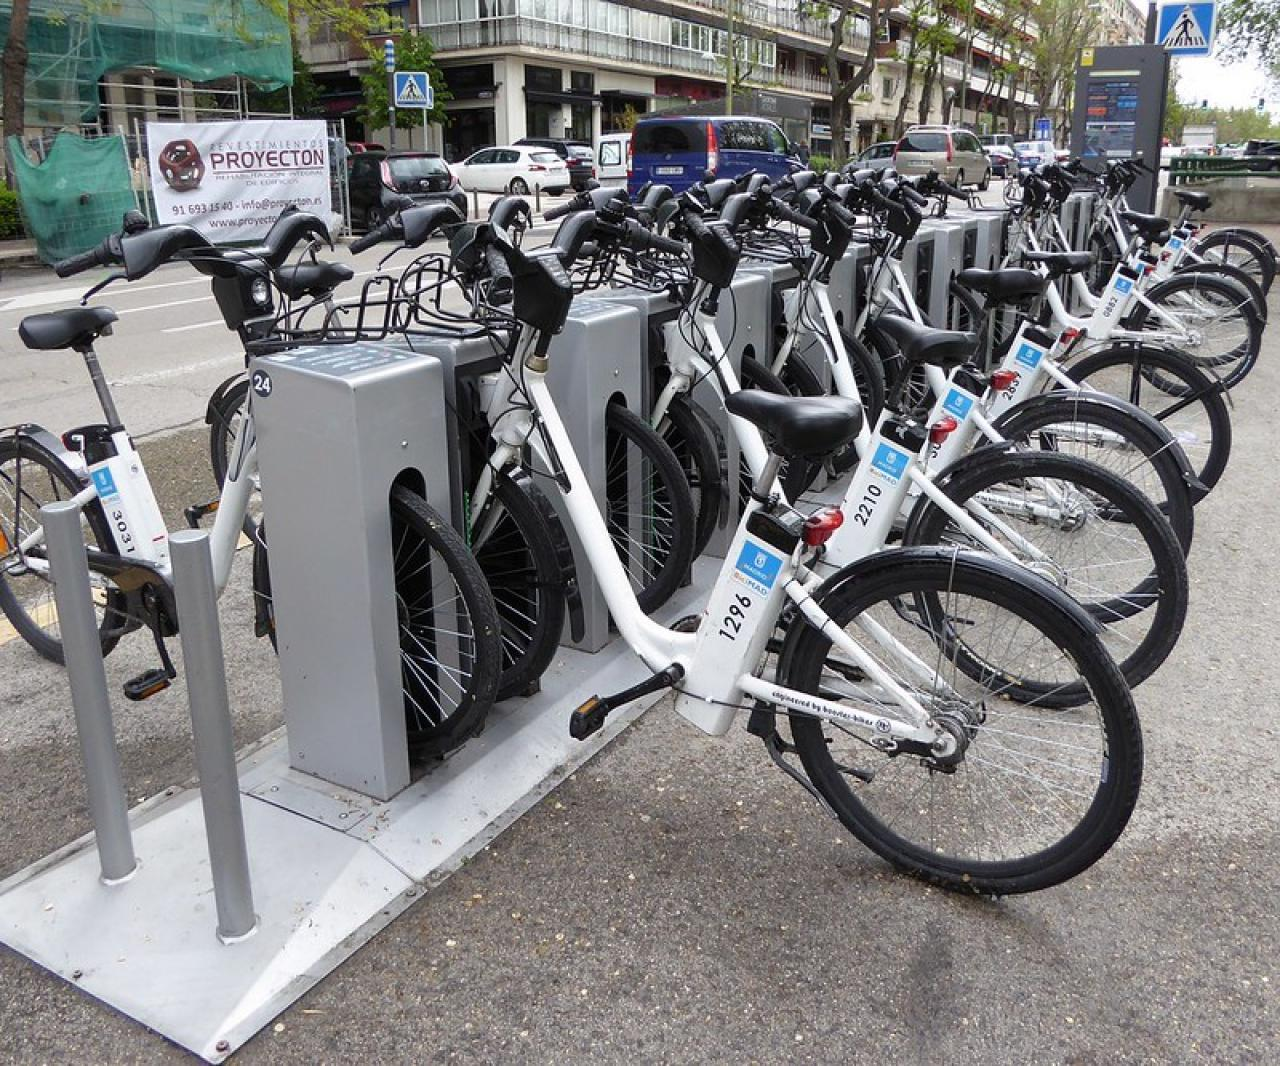
\includegraphics[scale=0.27]{Gambar FHO/e-bikes-madrid-licenced-under-cc-20-bicimad-flickr.jpg}
    \caption{Stasiun Sepeda Listrik (\protect\mycite{roadcc2021})}
    \label{Electric bike sharing}
\end{figure}

Sistem \textit{electric bike-sharing} merupakan evolusi dari sistem \textit{bike-sharing} konvensional yang menggabungkan keuntungan dari mobilitas aktif dengan teknologi \textit{electric assist} untuk memperluas jangkauan dan aksesibilitas layanan (\mycitet{fishman2020bikeshare}). Sepeda listrik dalam sistem ini umumnya dilengkapi dengan motor listrik yang membantu pengendara, terutama saat menghadapi tanjakan atau perjalanan jarak jauh, sehingga memperluas segmen pengguna potensial (\mycitet{campbell2016electric}).
Komponen kunci dari sistem \textit{electric bike-sharing} meliputi:
\begin{enumerate}
    \item \textbf{Sepeda Listrik}\\ Umumnya menggunakan sepeda dengan \textit{pedal-assist electric motor} dengan baterai yang dapat diisi ulang (\mycitet{ling2017emerging}).
    \item \textbf{Stasiun Pengisian}\\ Infrastruktur yang memungkinkan pengguna untuk mengambil dan mengembalikan sepeda serta mengisi daya baterai (\mycitet{sun2018data}).
    \item \textbf{Sistem Akses dan Pembayaran}\\ Mekanisme yang memungkinkan pengguna untuk mendaftar, membuka kunci sepeda, dan membayar layanan, biasanya melalui aplikasi smartphone atau kartu RFID (\mycitet{shaheen2019sharing}).
\end{enumerate}
Dibandingkan dengan sistem \textit{bike-sharing} konvensional, \textit{electric bike-sharing} menawarkan beberapa keunggulan:
\begin{enumerate}
    \item Dengan kemampuan sepeda listrik untuk menempuh jarak tempuh yang lebih jauh, memungkinkan pengguna untuk melakukan perjalanan yang lebih panjang (\mycitet{langford2013comparing}).
    \item Potensi untuk menggantikan perjalanan mobil jarak pendek hingga menengah yang berkontribusi pada pengurangan emisi (\mycitet{bikeplus2016shared}).
\end{enumerate}
Namun, sistem ini juga menghadapi tantangan di antaranya:
\begin{enumerate}
    \item Kebutuhan infrastruktur pengisian daya yang lebih kompleks terutama pada manajemen energi yang digunakan (\mycitet{sun2018data}).
    \item Biaya operasional yang lebih tinggi karena harga sepeda listrik dan pemeliharaan.
    \item Manajemen baterai, termasuk pengisian daya dan penggantian (\mycitet{ling2017emerging}).
\end{enumerate}
Optimalisasi lokasi stasiun pengisian daya menjadi krusial, mengingat biaya infrastruktur yang signifikan dan dampaknya terhadap aksesibilitas sistem. Model stokastik, seperti yang diusulkan oleh \mycite{brandstatter2017determining}, memungkinkan perencana untuk mempertimbangkan ketidakpastian permintaan dan variabilitas operasional dalam menentukan lokasi stasiun yang optimal.

Untuk merepresentasikan sistem \textit{bike-sharing} ini dibentuk kerangka kerja dengan menggunakan teori graf. Kerangka kerja ini dapat memodelkan konektivitas jaringan stasiun dan rute perjalanan sistem \textit{bike-sharing} dengan merepresentasikan stasiun sebagai titik dan rute trip-trip sebagai busur.

\section{Graf Berarah}
    Berikut diberikan definisi graf berarah.

\begin{definisi}
    digraf (directed graph) $G$ adalah pasangan himpunan tak kosong berhingga $V(G)$ dengan elemen-elemennya disebut titik (\textit{vertex}) dan himpunan berhingga $A(G)$ dengan elemennya merupakan pasangan berurutan $(u,v)$ dari dua titik berbeda $u$ dan $v$ di $V(G)$ yang disebut busur (arc). Pasangan himpunan titik $V(G)$ dan himpunan busur $A(G)$ dinotasikan dengan $G = (V(G), A(G))$. Untuk pasangan berurutan $(u,v)$, titik $u$ disebut titik awal dan titik $v$ disebut titik akhir dari busur tersebut.
\end{definisi}

Sebarang digraf dapat divisualisasikan dengan elemen di $V(G)$ digambarkan dalam bentuk titik/lingkaran dan elemen $(u,v)$ di $A(G)$ digambarkan sebagai busur dari $u$ ke $v$. Pada tulisan ini, penyebutan digraf akan disingkat dengan graf saja.

\begin{contoh}\label{contoh_digraph}
    Diberikan graf seperti berikut.\\
    \begin{figure}[H]
        \centering
        
\begin{tikzpicture}[scale = 0.8]
        \tikzset{vertexStyle/.append style = {shape=circle,fill=blue!10,minimum size=20pt,inner sep=1pt}}
        \Vertex[x=4.5, y=1.55,label=$C$]{C}
        \Vertex[x=3, y=0,label=$D$]{D}
        \Vertex[x=3, y=3,label=$A$]{A}
        \Vertex[x=6, y=3,label=$B$]{B}
        \Vertex[x=6, y=0,label=$E$]{E}
        \Edge[style={->}](A)(B)
        \Edge[style={->}](A)(C)
        \Edge[style={->}](D)(A)
        \Edge[style={->}](C)(E)
        \Edge[style={->}](B)(C)
        \Edge[style={->}](C)(D)
        \Edge[style={->}](B)(E) % Added arrow from E to B
        \end{tikzpicture}
        \caption{Digraf}
        \label{Digraph}
    \end{figure}

    Diperhatikan pada Gambar 2.3 terdapat digraf dengan himpunan titik yang terdiri dari $\{A,B,C,D,E\}$ dan himpunan busur yang terdiri dari $\{(A,B),(A,C),(D,A),(C,E),(B,C),(C,D),(E,B)\}$ dengan arah dalam busur ditunjukkan oleh panah. 
\end{contoh}

\begin{definisi}
     Diberikan graf $G=(V(G),A(G))$. \textit{Walk} didefinisikan sebagai barisan berhingga dari titik-titik $v_1, v_2, ..., v_m \in V(G)$ yang setiap dua titik berurutan terhubung oleh busur dan dinotasikan dengan $v_1 \rightarrow v_2 \rightarrow v_3 \rightarrow ... \rightarrow v_m$. Panjang \textit{walk} didefinisikan sebagai banyaknya busur yang dilewati dalam \textit{walk} tersebut. Selanjutnya, \textit{path} adalah \textit{walk} dengan semua titik dan busur yang dilewati berbeda. 
\end{definisi}

Untuk memperjelas perbedaan antara \textit{walk} dan \textit{path}, disajikan contoh berikut.
\begin{contoh}
    Pada Gambar \ref{Digraph} dapat dibentuk \textit{walk} $C\rightarrow D \rightarrow A \rightarrow B \rightarrow C \rightarrow E$ yang merupakan \textit{walk} dari $C$ menuju $E$ dengan panjang enam berdasarkan jumlah busur dalam \textit{walk}. Dapat dibentuk juga \textit{walk} $C \rightarrow D \rightarrow A \rightarrow B \rightarrow E$ yang merupakan \textit{path} karena titik dan busur dari \textit{walk} titik $C$ menuju titik $E$ masing-masing dilewati tepat sekali.
\end{contoh}

Dalam banyak aplikasi, termasuk dalam pemodelan sistem \textit{electric bike-sharing}, seringkali diperlukan pemberian nilai atau bobot pada busur dalam graf. Konsep ini dikenal sebagai graf berbobot yang didefinisikan sebagai berikut.
\begin{definisi}
    (\mycite{wilson1996introduction}) Bobot dari graf adalah nilai numerik yang diberikan untuk setiap busur pada graf. 
\end{definisi}

Bobot ini sering digunakan untuk merepresentasikan jarak, biaya, waktu, atau properti lain yang relevan dengan hubungan antara dua titik dalam graf. Untuk visualisasi konsep graf berbobot, disajikan contoh berikut.
\begin{contoh}
    Diberikan diagram graf seperti berikut.\\
    \begin{figure}[H]
        \centering
        
\begin{tikzpicture}[scale = 0.8]
        \tikzset{vertexStyle/.append style = {shape=circle,fill=blue!10,minimum size=20pt,inner sep=1pt}}
        \Vertex[x=4.5, y=1.55,label=$C$]{C}
        \Vertex[x=3, y=0,label=$D$]{D}
        \Vertex[x=3, y=3,label=$A$]{A}
        \Vertex[x=6, y=3,label=$B$]{B}
        \Vertex[x=6, y=0,label=$E$]{E}
        \Edge[label=1,bend=0](A)(B)
        \Edge[label=2,bend=0](A)(C)
        \Edge[label=3](A)(D)
        \Edge[label=2](B)(E)
        \Edge[label=3](C)(E)
        %\Edge[bend=-15](E)(B)
        \Edge[label=1](B)(D)
        \end{tikzpicture}
        \caption{Graf Berbobot}
        \label{Graf sederhana}
    \end{figure}

    Diperhatikan pada Gambar \ref{Graf sederhana}, terdapat nilai nonnegatif, yaitu $1,2,3$ secara acak di tiap busur. Nilai-nilai tersebut adalah bobot dari graf.
\end{contoh}

Pada permasalahan stokastik lokasi stasiun pengisian daya untuk \textit{electric bike-sharing}, titik potensial pembangunan stasiun pengisian daya dapat dipandang sebagai titik. Trip tiap skenario merupakan busur, rute perjalanan dalam skenario adalah \textit{path}, kontribusi profit tiap trip merepresentasikan bobot, dan digraf merupakan arah dari trip tiap skenario (\mycite{brandstatter2017determining}).
    
\section{Program Linear Bilangan Bulat}

Program linear bilangan bulat merupakan perluasan dari program linear yang memiliki batasan tambahan pada variabel keputusannya. Sebelum membahas lebih lanjut tentang program linear bilangan bulat, penting untuk memahami konsep dasar fungsi linear dan pertidaksamaan linear.

\begin{definisi}[\mycite{winston2004operations}]
    Suatu fungsi $f: \mathbb{R}^n \rightarrow \mathbb{R}$ disebut sebagai \textbf{fungsi linear} jika dan hanya jika terdapat vektor $\boldsymbol{c} = (c_1, c_2, ..., c_n) \in \mathbb{R}^n$ sehingga untuk setiap $\boldsymbol{x} = (x_1, x_2, ..., x_n) \in \mathbb{R}^n$, berlaku
    $$f(\boldsymbol{x}) = \boldsymbol{c^T x} = {c_1x_1 + c_2x_2 + ... + c_nx_n}.$$
\end{definisi}
Untuk memperjelas konsep fungsi linear, berikut disajikan contoh fungsi linear dan bukan fungsi linear.
\begin{contoh}
    Fungsi $f(x_1,x_2)=3x_1+2x_2$ merupakan fungsi linear dari $x_1$ dan $x_2$ karena fungsi tersebut dapat ditulis dalam bentuk $c_1x_1 + c_2x_2$ dengan $c_1 = 3$ dan $c_2 = 2$.
    Sebaliknya, fungsi $f(x_1,x_2)=x_1x_2^2$ bukan merupakan fungsi linear dari $x_1$ dan $x_2$ karena fungsi tersebut mengandung perkalian antara variabel ($x_1x_2$) dan variabel berpangkat ($x_2^2$) yang tidak sesuai dengan definisi fungsi linear.
\end{contoh}

Selanjutnya, konsep pertidaksamaan linear juga penting dalam pemrograman linear. Pertidaksamaan linear didefinisikan sebagai berikut.

\begin{definisi}[\mycite{winston2004operations}]
    Diberikan fungsi linear $f: \mathbb{R}^n \rightarrow \mathbb{R}$ dan $b \in \mathbb{R}$, \textbf{pertidaksamaan linear} dapat dinyatakan dalam bentuk $f(\textbf{x}) \leq b$ atau $f(\textbf{x}) \geq b$, dengan $\textbf{x} \in \mathbb{R}^n$
\end{definisi}

Untuk lebih memahami konsep pertidaksamaan linear, diberikan contoh berikut.
\begin{contoh}
    Pertidaksamaan $x_1+4x_2\leq 3$ dan $3x_1+x_2\geq 4$ merupakan pertidaksamaan linear. Sebaliknya, $x_1^3x_2\leq 5$ bukan merupakan pertidaksamaan linear karena mengandung $x_1^3$ dan perkalian antara variabel $x_1$ dan $x_2$.
\end{contoh}

Setelah memahami konsep fungsi linear dan pertidaksamaan linear, dapat didefinisikan masalah program linear.
    \begin{definisi}[\mycite{winston2004operations}]
    Masalah program linear (LP) adalah permasalahan optimisasi dengan kriteria berikut:
    \begin{enumerate}
        \item Memaksimalkan (atau meminimalkan) fungsi linear dari variabel keputusan. Fungsi tujuan ini disebut dengan fungsi objektif.
        \item Nilai dari variabel keputusan harus memenuhi kendala. Tiap kendala berbentuk persamaan linear dan atau pertidaksamaan linear.
        \item Batasan untuk tiap variabel. Untuk setiap variabel $\boldsymbol{x}$ didefinisikan batasan secara spesifik, yaitu $x_i$ nonnegatif $(x_i\geq 0)$ untuk setiap $i=1,2,\ldots, n$ atau tidak diberi batasan.
    \end{enumerate}

    Bentuk rumusan masalah \textbf{program linear (LP)} dapat dinyatakan dalam bentuk
    \begin{align*}
        \max/\min \quad & \boldsymbol{c}^T \boldsymbol{x}, \\
        \text{dengan kendala} \quad & \boldsymbol{Ax} \leq \boldsymbol{b}, \\
        & \boldsymbol{x} \geq 0,
    \end{align*}
    dengan $\textbf{x} \in \mathbb{R}^n$ adalah vektor variabel keputusan, $\textbf{c} \in \mathbb{R}^n$ adalah vektor koefisien fungsi tujuan, $\textbf{A} \in \mathbb{R}^{m \times n}$ adalah matriks koefisien kendala, dan $\textbf{b} \in \mathbb{R}^m$ adalah vektor batas kanan kendala.
\end{definisi}

Lebih lanjut diberikan contoh masalah program linear berikut.
\begin{contoh}
    Berikut adalah contoh program linear:
    $$
    \begin{aligned}
    \text{Maksimalkan} \quad & z = 3x_1 + 2x_2, \\
    \text{dengan kendala} \quad & x_1 + x_2 \leq 10, \\
    & 2x_1 + x_2 \leq 15, \\
    & x_1, x_2 \geq 0.
    \end{aligned}
    $$
    Dalam contoh ini:
    \begin{enumerate}
        \item Tujuan  masalah di atas adalah memaksimalkan fungsi objektif $z = 3x_1 + 2x_2$ yang akan dimaksimalkan.
        \item Terdapat dua kendala: $x_1 + x_2 \leq 10$ dan $2x_1 + x_2 \leq 15$.
        \item Terdapat batasan nonnegatif pada variabel: $x_1, x_2 \geq 0$.
    \end{enumerate}
\end{contoh}

Dalam program linear, konsep daerah fisibel sangat penting. Daerah fisibel didefinisikan sebagai berikut.
\begin{definisi}[\mycite{winston2004operations}]
Daerah fisibel masalah program linear adalah himpunan dari semua titik yang memenuhi semua kendala dan batasan variabel. Daerah fisibel dapat dinyatakan sebagai berikut
$$\mathcal{F} = \{\boldsymbol{x} \in \mathbb{R}^n : \boldsymbol{Ax} \leq \boldsymbol{b}, \boldsymbol{x} \geq 0\}.$$
\end{definisi}

Untuk memvisualisasikan konsep daerah fisibel, diperhatikan contoh berikut.
\begin{contoh}
    Pada Contoh 2.3.6, daerah fisibel adalah area yang dibatasi oleh:
    \begin{enumerate}
    \item garis $x_1 + x_2 = 10$,
        \item garis $2x_1 + x_2 = 15$,
        \item sumbu $x_1$ (karena $x_2 \geq 0$), dan
        \item sumbu $x_2$ (karena $x_1 \geq 0$).
    \end{enumerate}
    Daerah ini membentuk suatu poligon dalam bidang $x_1x_2$.
    
    \begin{figure}[H]
        \centering
        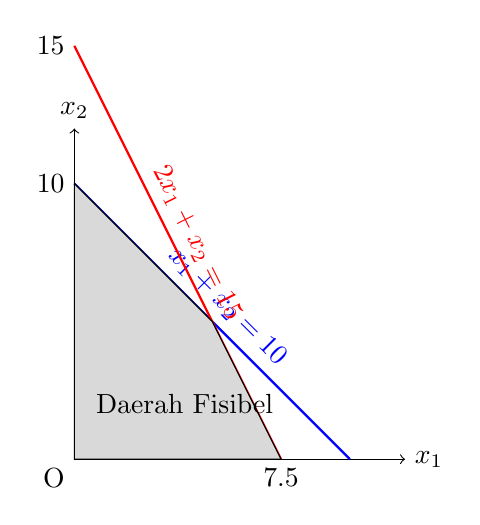
\begin{tikzpicture}[scale=0.35]
        \draw[->] (0,0) -- (12,0) node[right] {$x_1$};
        \draw[->] (0,0) -- (0,12) node[above] {$x_2$};
        \draw[thick, blue] (0,10) -- (10,0) node[midway, above, sloped] {$x_1 + x_2 = 10$};
        \draw[thick, red] (0,15) -- (7.5,0) node[midway, above, sloped] {$2x_1 + x_2 = 15$};
        
        \filldraw[fill=gray!30, draw=black] (0,0) -- (0,10) -- (5,5) -- (7.5,0) -- cycle;
        
        \node[below left] at (0,0) {O};
        \node[below] at (7.5,0) {7.5};
        \node[left] at (0,10) {10};
        \node[left] at (0,15) {15};
        
        \node at (4,2) {Daerah Fisibel};
        \end{tikzpicture}
        \caption{Daerah Fisibel untuk Contoh 2.3.6}
        \label{fig:feasible_region}
    \end{figure}
\end{contoh}

Setelah memahami daerah fisibel, dapat didefinisikan solusi optimal dari program linear.
\begin{definisi}[\mycite{winston2004operations}]
    Untuk masalah memaksimalkan, solusi optimal $\hat{x}$ dari program linear adalah
    $$\boldsymbol{\hat{x}} = \arg\max_{\boldsymbol{x} \in \mathcal{F}} \boldsymbol{c}^T \boldsymbol{x}$$
    dengan $\mathcal{F}$ adalah daerah fisibel dan $\arg\max$ (argumen maksimum) menunjukkan nilai $\boldsymbol{x}$ dalam $\mathcal{F}$ yang menghasilkan nilai maksimum dari fungsi objektif $\boldsymbol{c}^T \boldsymbol{x}$.
\end{definisi}

Untuk lebih memahami konsep solusi optimal, diperhatikan contoh berikut.
\begin{contoh}
    Dalam program linear pada contoh sebelumnya, solusi optimal akan berada pada salah satu titik sudut dari daerah fisibel. Misalkan solusi optimalnya adalah $(x_1, x_2) = (5, 5)$, maka nilai fungsi objektif maksimalnya adalah $z = 3(5) + 2(5) = 25$.
\end{contoh}

Sistem \textit{electric bike-sharing} erat berkaitan dengan program bilangan bulat karena sistem ini dibentuk dengan menentukan variabel-variabel keputusan dalam bilangan bulat seperti pembangunan stasiun potensial maupun jumlah armada sepeda yang dibutuhkan. Selanjutnya, didefinisikan program bilangan bulat.

\begin{definisi}[\mycite{winston2004operations}]
    Masalah \textbf{program bilangan bulat (IP)} adalah masalah program linear dengan tambahan kendala bahwa beberapa atau semua variabel harus berupa bilangan bulat. Bentuk umum masalah program bilangan bulat adalah
    \begin{align*}
        \max/\min \quad & \boldsymbol{c}^T \boldsymbol{x}, \\
        \text{dengan kendala} \quad & \boldsymbol{Ax} \leq \boldsymbol{b}, \\
        & \boldsymbol{x} \geq 0,\\
        & x_i \in \mathbb{Z}, \quad \text{untuk beberapa atau semua } i.
    \end{align*}
\end{definisi}

Untuk lebih memahami berbagai jenis program bilangan bulat, diperhatikan contoh berikut.
\begin{contoh}
    Berikut adalah contoh program bilangan bulat murni.
    $$\begin{aligned}
        \text{Maksimalkan} \quad & z = 3x_1 + 2x_2, \\
        \text{dengan kendala} \quad & x_1 + x_2 \leq 6, \\
        & x_1, x_2 \geq 0, \\
        & x_1, x_2 \in \Z.
    \end{aligned}$$
    Contoh program bilangan bulat campuran.
    $$\begin{aligned}
        \text{Maksimalkan} \quad & z = 3x_1 + 2x_2 ,\\
        \text{dengan kendala} \quad & x_1 + x_2 \leq 6, \\
        & x_1, x_2 \geq 0 ,\\
        & x_1 \in \Z.
    \end{aligned}$$
    Contoh IP 0-1.
    $$\begin{aligned}
        \text{Maksimalkan} \quad & z = x_1 - x_2,\\
        \text{dengan kendala} \quad & x_1 + 2x_2,\leq 2 \\
        & 2x_1 - x_2 \leq 1, \\
        & x_1, x_2 = 0 \text{ atau } 1.
    \end{aligned}$$
\end{contoh}

Dalam konteks \textit{electric bike-sharing}, program bilangan bulat dapat digunakan untuk menentukan jumlah stasiun yang harus dibangun (variabel bilangan bulat) dan kapasitas masing-masing stasiun (variabel bilangan bulat), sambil memaksimalkan cakupan layanan atau meminimalkan biaya total.

\section{Proses Stokastik dan Probabilitas}
Dalam kejadian apapun di dunia ini dapat dibedakan menjadi kepastian, ketidakpastian, dan kemustahilan. Misalkan, pasti semua sepeda listrik membutuhkan baterai untuk beroperasi,  kemungkinan orang lebih menggunakan sepeda listrik pada hari kerja, ataupun tidak mungkin sepeda listrik berubah menjadi mobil dalam perjalanan. Berdasarkan permisalan sederhana ini, dapat didefinisikan konsep \textit{randomness}.

Konsep \textit{randomness} erat kaitannya dengan probabilitas yang merupakan alat matematis untuk mengukur dan menganalisis kejadian-kejadian acak. Probabilitas memungkinkan untuk mengkuantifikasi ketidakpastian dan membuat prediksi dalam situasi yang tidak deterministik. Untuk memahami probabilitas dengan lebih baik, perlu diketahui beberapa konsep dasar (\mycite{ross2014introduction}).

% \begin{definisi} (\mycite{ross2014introduction})
%     Probabilitas adalah ukuran numerik dari kemungkinan terjadinya suatu kejadian. Nilai probabilitas berada antara 0 dan 1 dengan 0 menunjukkan kejadian yang mustahil terjadi dan 1 menunjukkan kejadian yang pasti terjadi.
% \end{definisi}

Untuk memahami bagaimana probabilitas berlaku, perlu didefinisikan ruang sampel.

\begin{definisi}(\mycite{ross2014introduction})
    Ruang sampel ($\Omega$) adalah himpunan semua hasil yang mungkin dari suatu eksperimen acak.
\end{definisi}

Setelah memahami ruang sampel, dapat didefinisikan fungsi probabilitas yang memetakan kejadian dalam ruang sampel ke nilai probabilitasnya.

\begin{definisi}
    (\mycite{billingsley1995probability}) Probabilitas $P$ adalah fungsi yang memetakan setiap kejadian $A$ dalam ruang sampel $\Omega$ ke suatu bilangan real antara 0 dan 1 yang memenuhi sifat-sifat berikut :
    \begin{enumerate}
        \item $P(A) \geq 0$ untuk setiap kejadian $A$.
        \item $P(\Omega) = 1$.
        \item Untuk kejadian-kejadian yang saling lepas $A_1, A_2, ...$, berlaku $P(\bigcup_{i=1}^{\infty} A_i) = \sum_{i=1}^{\infty} P(A_i)$.
    \end{enumerate}
\end{definisi}

Dalam program stokastik yang akan dijelaskan kemudian, erat kaitannya dengan variabel-variabel acak. Berikut didefinisikan variabel acak.

\begin{definisi}(\mycite{ross2014introduction})
    Variabel acak adalah fungsi yang memetakan setiap hasil dalam ruang sampel ke suatu bilangan real, dinotasikan dengan $X(c)=x$ dengan $c \in \Omega$ dan $x\in \mathbb{R}$
\end{definisi}

Variabel acak terbagi menjadi dua yaitu variabel acak diskrit dan variabel acak kontinu, variabel acak diskrit akan didefinisikan sebagai berikut.

\begin{definisi}(\mycite{casella2002statistical})
    Variabel acak diskrit adalah variabel acak yang hanya dapat mengambil dalam himpunan terhitung. Fungsi probabilitas dari variabel acak diskrit $X$ didefinisikan sebagai $p(x) = P(X = x)$ untuk setiap nilai $x$ yang mungkin dari $X$, dan $p(x)$ memenuhi sifat:
    \begin{enumerate}
        \item $p(x)\geq0$ untuk semua $x$,
        \item $\sum_x p(x)=1$.
    \end{enumerate}
\end{definisi}

Selanjutnya variabel acak kontinu akan didefinisikan sebagai berikut.

\begin{definisi}(\mycite{ross1996stochastic})
    Variabel acak kontinu adalah variabel acak yang dapat mengambil nilai pada suatu interval bilangan real. Variabel acak kontinu $X$ ditandai dengan fungsi kepadatan probabilitas $f(x)$, dengan probabilitas $X$ berada pada interval $[a,b]$ didefinisikan
    
    $$P(a \leq X \leq b) = \int_a^b f(x) dx,$$

    \noindent dan $f(x)$ memenuhi sifat:
    \begin{enumerate}
        \item $f(x) \geq 0$ untuk semua $x$,
        \item $\int_{-\infty}^{\infty} f(x) dx = 1$.
    \end{enumerate}
\end{definisi}

Salah satu cara untuk mendapatkan makna dari variabel-variabel acak ini adalah dengan mencari nilai ekspektasinya yang umum dalam formulasi program stokastik. Berikut didefinisikan nilai ekspektasi.

\begin{definisi}(\mycite{casella2002statistical})
    Nilai harapan atau ekspektasi dari variabel acak $X$ dengan fungsi probabilitas $p(x)$ didefinisikan sebagai
    
    \begin{align*}
        E[X] &= \sum_{x} x \cdot p(x), \quad X \text{ variabel acak diskrit}, \\
        \text{dan}\\
        E[X] &= \int x \cdot f(x) \, dx, \quad X \text{ variabel acak kontinu}.
    \end{align*}
\end{definisi}

Dalam konteks permasalahan stokastik lokasi stasiun pengisian daya untuk \textit{electric bike-sharing}, konsep probabilitas dan nilai harapan sangat penting. Permintaan pengguna sepeda listrik dapat dianggap sebagai variabel acak dan dapat digunakan nilai harapan untuk memperkirakan permintaan rata-rata pada setiap stasiun.

\begin{definisi}(\mycite{ross1996stochastic})
    Proses stokastik adalah kumpulan variabel acak $X(t)$, $t\in T$ yang diindekskan oleh parameter $t$ yang merepresentasikan waktu.
\end{definisi}

Dalam sistem \textit{electric bike-sharing}, permintaan sepeda listrik di setiap stasiun dapat dimodelkan sebagai proses stokastik yang mana permintaan bervariasi seiring waktu dan dipengaruhi oleh berbagai faktor acak seperti cuaca, hari dalam seminggu, atau acara khusus di sekitar lokasi sebagai contoh berikut.

\begin{contoh}
    Dalam sistem \textit{electric bike-sharing}, permintaan sepeda listrik di setiap stasiun dapat dimodelkan sebagai proses stokastik. Misalkan $X(t)$ mewakili jumlah permintaan sepeda listrik pada waktu $t$ di suatu stasiun tertentu. Proses stokastik ini mungkin terlihat seperti berikut.
    \begin{enumerate}
        \item $X(9:00) = 5$ (5 permintaan pada pukul 9:00),
        \item $X(10:00) = 8$ (8 permintaan pada pukul 10:00), dan
        \item $X(11:00) = 3$ (3 permintaan pada pukul 11:00).
    \end{enumerate}
\end{contoh}

Dalam pemodelan kedatangan pelanggan atau permintaan, sering digunakan distribusi Poisson. Distribusi Poisson sering digunakan untuk memodelkan kedatangan pelanggan dalam sistem antrian yang dapat diterapkan dalam konteks permintaan sepeda listrik di stasiun-stasiun pengisian daya (\mycite{grimmett2020probability}).

\begin{definisi}(\mycite{haight1967handbook})
    Distribusi Poisson adalah distribusi probabilitas diskret yang mengekspresikan probabilitas sejumlah kejadian terjadi dalam interval waktu atau ruang tertentu jika kejadian-kejadian tersebut terjadi dengan rata-rata yang diketahui dan independen terhadap waktu sejak kejadian terakhir. Fungsi massa probabilitas dari distribusi Poisson didefinisikan dengan 
    \begin{align*}
        P(X=k) = \frac{e^{-\lambda}\lambda^k}{k!}, k = 0, 1, 2, \ldots.
    \end{align*}
\end{definisi}

Selanjutnya, akan diberikan contoh dari penerapan distribusi Poisson.

\begin{contoh}
    Misalkan rata-rata kedatangan pelanggan di suatu stasiun \textit{electric bike-sharing} adalah empat orang per jam. Jika kedatangan pelanggan mengikuti distribusi Poisson, maka probabilitas tepat $k$ pelanggan datang dalam satu jam diberikan oleh
    $$P(X = k) = \frac{e^{-\lambda}\lambda^k}{k!}$$
    dengan $\lambda = 4$ (rata-rata kedatangan per jam) dan $k$ adalah jumlah kedatangan yang ingin dihitung probabilitasnya.
    Oleh karena itu, probabilitas tepat tiga pelanggan datang dalam satu jam adalah
    $$P(X = 3) = \frac{e^{-4}4^3}{3!} \approx 0.195.$$
    Ini berarti terdapat tepat tiga pelanggan akan datang dalam satu jam di stasiun tersebut dengan probababilitas sebesar 0.195.
\end{contoh}



\section{Teori Optimisasi}

Optimisasi adalah proses menemukan solusi terbaik dari suatu masalah di bawah kondisi tertentu. Dalam \textit{electric bike-sharing}, optimisasi berperan penting dalam menentukan lokasi stasiun pengisian daya yang optimal, alokasi sepeda, dan manajemen sistem secara keseluruhan. Berikut beberapa konsep utama yang relevan dalam penulisan ini.
\begin{definisi}(\mycite{nocedal2006numerical})
Diberikan masalah optimisasi
\begin{center}
    $\min_{\boldsymbol{x} \in X} f(\boldsymbol{x})$,
\end{center}
    dengan $X \subseteq \mathbb{R}^n$ adalah himpunan fisibel dan $f: X \rightarrow \mathbb{R}$ adalah fungsi tujuan. Suatu titik $\boldsymbol{x^*} \in X$ disebut solusi global jika $f(\boldsymbol{x^*}) \leq f(\boldsymbol{x})$ untuk semua $\boldsymbol{x} \in X$.
\end{definisi}
Dalam masalah penentuan lokasi stasiun pengisian daya, solusi global direpresentasikan dengan konfigurasi terbaik dari variabel keputusan sebagai contoh, konfigurasi yang dimaksud meliputi penentuan lokasi-lokasi spesifik untuk stasiun pengisian daya guna memaksimalkan keuntungan atau meminimalkan biaya secara keseluruhan.  Dalam penyelesaian model yang kompleks seperti ini dapat digunakan algoritma metaheuristik sebagai alat untuk menemukan solusi terbaik dan untuk menemukan solusi terbaik ini terlebih dahulu dicari dalam ruang pencarian.

\begin{definisi} (\mycite{glover1986future})
    Ruang pencarian $S$ adalah himpunan semua solusi yang mungkin untuk suatu masalah optimisasi. Setiap elemen $s \in S$ merepresentasikan satu konfigurasi susunan nilai variabel-variabel keputusan atau solusi potensial dari masalah yang sedang diselesaikan.
\end{definisi}

Ruang pencarian memberikan gambaran tentang semua kemungkinan solusi yang dapat dieksplorasi oleh algoritma optimisasi. Kemudian, untuk lebih memperjelas struktur ruang pencarian diperlukan fungsi \textit{neighbourhood}.

\begin{definisi} (\mycite{glover1986future})
    Fungsi neighborhood $N: S \rightarrow 2^S$ adalah fungsi yang memetakan setiap solusi $s \in S$ ke subset dari $S$ yang disebut neighborhood dari $s$. Elemen-elemen dalam $N(s)$ biasanya merupakan solusi yang dapat dicapai dari $s$ melalui modifikasi kecil atau operasi tertentu.
\end{definisi}

Berikut diberikan contoh dari fungsi \textit{neighbourhood}.

\begin{contoh}
    Misalkan sebuah sistem bike-sharing memiliki dua stasiun, masing-masing dengan kapasitas maksimal 5 sepeda. Suatu solusi direpresentasikan oleh pasangan bilangan $(x, y)$, dengan $x$ adalah jumlah sepeda di stasiun 1 dan $y$ adalah jumlah sepeda di stasiun 2.
    
    Fungsi \textit{neighborhood} $N(s)$ untuk solusi $s = (x, y)$ dapat dibentuk sebagai berikut.
    \[
    N(x, y) = \{(x', y') \mid |x' + y' - (x + y)| \leq 1, \, 0 \leq x' \leq 5, \, 0 \leq y' \leq 5\}
    \]
    \begin{enumerate}
        \item Solusi \textit{neighbor} adalah solusi yang dapat dicapai dengan memindahkan satu sepeda antar stasiun atau menambah/mengurangi satu sepeda dari sistem.
        \item Batasan $|x' + y' - (x + y)| \leq 1$ memastikan perubahan total sepeda tidak lebih dari 1.
        \item Batasan $0 \leq x' \leq 5$ dan $0 \leq y' \leq 5$ memastikan kapasitas stasiun tidak dilampaui.
    \end{enumerate}
    Diambil 2 pasangan kapasitas sepeda di stasiun 1 dan 2 sebagai berikut.
    \begin{enumerate}
        \item Jika $s = (3, 2)$, maka $N(s) = \{(2, 2), (3, 1), (3, 3), (4, 2), (2, 3), (4, 1)\}$,
        \item Jika $s = (5, 0)$, maka $N(s) = \{(4, 0), (4, 1), (5, 1)\}$.
    \end{enumerate}
\end{contoh}

Fungsi \textit{neighbourhood} ini memungkinkan algoritma optimisasi terutama metaheuristik untuk menjelajahi ruang pencarian secara efisien.

\begin{definisi} (\mycite{glover1986future})
    Metaheuristik adalah prosedur pencarian yang menggunakan strategi untuk mengeksplorasi ruang pencarian. Didefinisikan tupel $(S, f, N, M)$ dengan:
    \begin{enumerate}
    \item $S$ adalah ruang pencarian,
    \item $f: S \rightarrow \mathbb{R}$ adalah fungsi tujuan yang akan dioptimalkan,
    \item $N: S \rightarrow 2^S$ adalah fungsi neighborhood, dan
    \item $M$ adalah memori yang menyimpan informasi pencarian.
    \end{enumerate}
    Prosedur metaheuristik secara umum mencari nilai $s^* \in S$ sedemikian sehingga $f(s^*)$ optimal.
\end{definisi}

Algoritma \textit{Fire Hawk Optimizer} yang digunakan dalam penelitian ini termasuk dalam kategori metaheuristik.

\begin{contoh}
Misalkan dibentuk tupel $(S, f, N, M)$ sebagai berikut
\begin{enumerate}
    \item Himpunan $S$ adalah ruang pencarian yang terdiri dari semua konfigurasi yang mungkin untuk penempatan stasiun dan alokasi sepeda. Misalnya, $\boldsymbol{s} \in S$ mungkin direpresentasikan sebagai vektor $\boldsymbol{s} = (x_1, ..., x_n, y_1, ..., y_n)$, dengan $x_i$ adalah lokasi stasiun ke-$i$ dan $y_i$ adalah jumlah sepeda di stasiun tersebut.
    
    \item Fungsi $f: S \rightarrow \mathbb{R}$, merepresentasikan total keuntungan yang dinyatakan dalam 
    $$f(\boldsymbol{s}) = \sum_{i=1}^n (p_i y_i - c_i x_i) - \sum_{u \in U} \alpha_u d_u(\boldsymbol{s})$$
    dengan $p_i$ adalah profit per sepeda di stasiun $i$, $c_i$ adalah biaya pembangunan stasiun $i$, $\alpha_u$ adalah probabilitas skenario permintaan $u$, dan $d_u(\boldsymbol{s})$ adalah fungsi yang mengukur ketidakpuasan permintaan untuk konfigurasi $\boldsymbol{s}$ dalam skenario $u$.
    
    \item Fungsi $N: S \rightarrow 2^S$ adalah fungsi neighborhood yang mendefinisikan solusi-solusi yang dapat dicapai dari suatu solusi dengan modifikasi. Misalnya,
    \begin{align*}
        N(\boldsymbol{s}) = \{\boldsymbol{s'} \in S \mid \boldsymbol{s'} \text{ didapat dengan memilih stasiun} \\
        \phantom{N(s) = \{s' \in S \mid} \text{atau mengubah alokasi sepeda}\}
    \end{align*}
    
    \item Notasi $M$ merupakan struktur memori yang menyimpan informasi pencarian, seperti solusi terbaik yang ditemukan sejauh ini, frekuensi pencarian ke area tertentu dalam ruang pencarian, atau tren perubahan fungsi tujuan.
\end{enumerate}

Tujuan dari metaheuristik ini adalah menemukan nilai $\boldsymbol{s^*} \in S$ yang memaksimalkan $f(\boldsymbol{s})$. Seperti halnya algoritma \textit{fire hawk optimizer} terdiri dari struktur ini untuk mengeksplorasi ruang pencarian $S$, mengevaluasi solusi $f$, menggunakan $N$ untuk bergerak antar solusi, dan memanfaatkan $M$ untuk menyimpan dan menggunakan informasi selama proses pencarian.

\end{contoh}

\chapter{OPTIMISASI STOKASTIK}

\section{Program Stokastik}
Dalam konteks optimisasi, terdapat dua jenis model utama, yaitu model deterministik dan model stokastik. Perbedaan mendasar antara keduanya terletak pada cara keduanya menangani ketidakpastian dalam parameter. Model deterministik mengasumsikan bahwa semua parameter diketahui secara pasti, meskipun dalam kenyataannya, nilai-nilai tersebut sering kali hanya berupa estimasi. Model ini memperlakukan parameter sebagai nilai tetap dan pasti, yang memudahkan proses optimisasi namun mungkin tidak sepenuhnya merefleksikan kondisi dunia nyata, di mana ketidakpastian selalu ada. Sebaliknya, model stokastik dirancang untuk mengakomodasi ketidakpastian dengan memodelkan setidaknya satu parameter sebagai variabel acak yang mengikuti distribusi probabilitas tertentu. Pendekatan stokastik memungkinkan analisis yang lebih realistis terhadap kondisi dunia nyata, terutama ketika menghadapi variabel yang tidak sepenuhnya dapat diprediksi.(\mycite{birge2011introduction}).

\begin{definisi} (\mycite{birge2011introduction})
    Program stokastik adalah model optimisasi di mana setidaknya satu dari parameter merupakan variabel acak.
\end{definisi}

Dengan mempertimbangkan ketidakpastian dalam model, program stokastik bertujuan untuk menemukan solusi yang optimal tidak hanya untuk satu skenario tunggal, tetapi juga untuk berbagai skenario yang mungkin terjadi. Pendekatan ini sangat relevan dalam konteks sistem \textit{electric bike-sharing}, di mana faktor-faktor seperti permintaan pengguna, ketersediaan sepeda, dan pasokan daya dapat berfluktuasi secara acak. Dengan mengakomodasi variasi ini, program stokastik dapat menghasilkan keputusan yang lebih adaptif dan robust, sehingga sistem dapat beroperasi secara optimal meskipun terdapat perubahan atau ketidakpastian di lapangan.

Selanjutnya, akan diberikan contoh permasalahan sederhana pemodelan program stokastik sebagai berikut.

\begin{contoh}
    Diberikan masalah optimisasi stokastik sederhana dengan variabel keputusan $\boldsymbol{x}$ dan variabel acak $\boldsymbol{c}$ yang memiliki fungsi objektif:
    $$
    \max E[\boldsymbol{c} \cdot \boldsymbol{x}]
    $$
    dengan kendala
    $$
    \boldsymbol{c} \in \mathbb{R}, \quad 0 \leq \boldsymbol{x} \leq 3, \quad \boldsymbol{x} \in \mathbb{Z}^n, \quad n \in \mathbb{N}.
    $$
    
    Notasi $E[\cdot]$ merepresentasikan nilai harapan, dengan fungsi objektif menggunakan ekspektasi $E[\boldsymbol{c} \cdot \boldsymbol{x}]$ karena $\boldsymbol{c}$ merupakan variabel acak yang mengikuti suatu distribusi probabilitas. Penggunaan ekspektasi ini memungkinkan perhitungan nilai rata-rata dari semua kemungkinan nilai $\boldsymbol{c}$, sehingga akan menghasilkan solusi yang optimal secara rata-rata.
    
    Misalkan $\boldsymbol{c}$ memiliki tiga kemungkinan nilai dengan distribusi diskrit,
    \begin{enumerate}
        \item $P(c = 2) = 0.2$,
        \item $P(c = 3) = 0.5$, dan
        \item $P(c = 4) = 0.3$.
    \end{enumerate}   
    Maka nilai ekspektasi dari $\boldsymbol{c}$ dapat dihitung sebagai
    $$E[\boldsymbol{c}] = 2 \cdot 0.2 + 3 \cdot 0.5 + 4 \cdot 0.3 = 3.1,$$
    sehingga fungsi objektif dapat ditulis menjadi
    $$E[\boldsymbol{c} \cdot \boldsymbol{x}] = 3.1x.$$
    
    Dengan demikian, meskipun nilai $\boldsymbol{c}$ bersifat tidak pasti, masalah optimisasi dapat diselesaikan dengan menggunakan nilai ekspektasinya untuk mendapatkan solusi yang optimal secara rata-rata.
\end{contoh}

\subsection{Program Bilangan Bulat Stokastik}
Program bilangan bulat stokastik mengembangkan konsep program stokastik dengan membatasi beberapa atau semua variabel keputusan menjadi bilangan bulat. Pendekatan ini sangat umum dalam aplikasi praktis, di mana keputusan harus dibuat dalam unit diskrit yang tidak dapat dibagi, seperti jumlah sepeda listrik yang harus disediakan dalam sistem \textit{electric bike-sharing}.

\begin{definisi}(\mycite{birge2011introduction})
    Program bilangan bulat stokastik adalah jenis program stokastik di mana solusi untuk salah satu atau lebih variabel keputusan harus berupa bilangan bulat.
\end{definisi}

Program bilangan bulat stokastik sangat relevan dengan \textit{electric bike-sharing} karena banyak keputusan yang harus diambil melibatkan variabel diskrit, seperti jumlah sepeda atau stasiun pengisian daya. Selain itu, ketidakpastian dalam permintaan dan biaya operasional menambah kompleksitas pada masalah optimisasi. Berikut diilustrasikan contoh penerapan program bilangan bulat stokastik.

\begin{contoh}
    Dimisalkan perusahaan \textit{electric bike-sharing} yang harus memutuskan jumlah sepeda listrik untuk dipesan menghadapi permintaan yang tidak pasti. Misalkan $\boldsymbol{x}$ adalah jumlah sepeda yang dipesan, $\boldsymbol{d}$ adalah permintaan (variabel acak), dan $p$ adalah keuntungan per sepeda yang disewakan. Oleh karena itu, masalah dapat diformulasikan sebagai
    $$
    \max E[\min(\boldsymbol{x}, \boldsymbol{d}) \cdot p] - c\boldsymbol{x}
    $$
    dengan kendala
    $$\boldsymbol{x} \geq 0, \quad \boldsymbol{x} \in \mathbb{Z}^n, \quad n \in \mathbb{N}.
    $$
    Konstanta $c$ menyatakan biaya tetap pemesanan satu unit sepeda listrik. Model ini mengoptimalkan keuntungan yang diharapkan dengan mempertimbangkan ketidakpastian dalam permintaan dan membuat keputusan tentang jumlah pesanan yang optimal sebagai variabel keputusan bilangan bulat.\\
    
    Model semacam ini sangat relevan dengan \textit{electric bike-sharing} di mana perusahaan harus memutuskan berapa banyak sepeda listrik yang harus dibeli di hadapan ketidakpastian mengenai permintaan pengguna dan biaya operasional yang bervariasi.
\end{contoh}

\subsection{Program Stokastik Dua Tahap}

Program stokastik dua tahap adalah salah satu jenis program stokastik yang memodelkan keputusan yang harus dibuat dalam dua tahap. Pada tahap pertama, keputusan diambil sebelum ketidakpastian (variabel acak) terungkap. Pada tahap kedua, setelah ketidakpastian diketahui, variabel keputusan tambahan dibuat untuk menyesuaikan atau merespons terhadap realisasi ketidakpastian tersebut (\mycite{birge2011introduction}).

\begin{definisi}(\mycite{birge2011introduction})
    \textbf{Program stokastik dua tahap} atau \textit{two stage stochastic programming} adalah model optimisasi dengan keputusan dapat dibagi dalami 2 fase atau tahap. Tahap pertama mempertimbangkan keputusan yang dibuat sebelum nilai dari variabel acak diketahui, dan tahap kedua memberikan respon setelah nilai parameter stokastik diketahui.
\end{definisi}

Untuk memperjelas konsep program stokastik dua tahap diilustrasikan contoh bagaimana keputusan dibagi menjadi dua tahap dan bagaimana ketidakpastian mempengaruhi proses pengambilan keputusan.

\begin{contoh}
    Misalkan sebuah operator \textit{electric bike-sharing} di Yogyakarta memiliki 2 jenis sepeda listrik, reguler dan premium. Setiap malam, operator harus memutuskan berapa jam operasional dari masing-masing jenis sepeda yang harus disiapkan di stasiun utama untuk keesokan harinya. Satu jam tambahan juga akan disediakan untuk fleksibilitas. Jika keesokan hari cuaca cerah (kemungkinan 70\%), akan ada permintaan untuk 3 jam sepeda reguler dan 1 jam sepeda premium. Jika cuaca hujan (kemungkinan 30\%), permintaan akan menjadi 1 jam sepeda reguler dan 3 jam sepeda premium. Operator ingin memaksimalkan ekspektasi total jam sepeda yang digunakan.

    Permasalahan ini adalah contoh program stokastik dua tahap. Pada tahap pertama, operator memutuskan alokasi awal jam operasional sepeda sebelum mengetahui kondisi cuaca. Tahap kedua terjadi keesokan hari ketika cuaca diketahui, dan operator dapat menyesuaikan alokasi jam operasional yang tersisa.

    Variabel keputusan tahap pertama adalah jumlah jam operasional sepeda reguler ($x_1$) dan premium ($x_2$) yang disiapkan. Untuk tahap kedua, $w_1^s$ dan $w_2^s$ adalah jumlah jam operasional sepeda reguler dan premium yang ditambahkan setelah cuaca diketahui, dengan $s = 1$ untuk cerah dan $s = 2$ untuk hujan. Variabel $z_1^s$ dan $z_2^s$ adalah jumlah jam operasional sepeda reguler dan premium yang digunakan pada hari dengan cuaca tipe $s$.
    
    Model program linear stokastik dua tahap dapat dinyatakan dalam bentuk
    
    $$
    \max \, 0{,}70 (z_1^1 + z_2^1) + 0{,}30 (z_1^2 + z_2^2)
    $$
    
    dengan kendala
    
    $$
    \begin{aligned}
    & x_1 + x_2 = 3, \\
    & x_1 + w_1^1 \geq z_1^1, \\
    & x_2 + w_2^1 \geq z_2^1, \\
    & w_1^1 + w_2^1 = 1, \\
    & z_1^1 \leq 3, \\
    & z_2^1 \leq 1, \\
    & x_1 + w_1^2 \geq z_1^2, \\
    & x_2 + w_2^2 \geq z_2^2, \\
    & w_1^2 + w_2^2 = 1, \\
    & z_1^2 \leq 1, \\
    & z_2^2 \leq 3, \\
    & \text{semua variabel} \geq 0.
    \end{aligned}
    $$
    
    Dengan menggunakan \textit{software} optimisasi Lingo 19.0 diperoleh solusi 2 jam operasional untuk sepeda reguler dan 1 jam untuk premium di malam hari. Jika cuaca cerah, operator menambahkan 1 jam operasional untuk sepeda reguler, sehingga jam operasional yang digunakan adalah 3 jam reguler dan 1 jam premium. Jika cuaca hujan, operator menambahkan 1 jam operasional untuk sepeda premium, sehingga jam operasional yang digunakan adalah 2 jam reguler dan 2 jam premium. Strategi ini menghasilkan ekspektasi penggunaan sebesar 3,7 jam per hari.
    
    Contoh ini mengilustrasikan bagaimana operator \textit{electric bike-sharing} dapat mengoptimalkan alokasi jam operasional sepeda dengan mempertimbangkan ketidakpastian cuaca dan pola permintaan untuk efisiensi operasional dan kepuasan pengguna.
    \label{contoh3.1.7}
\end{contoh}


\section{\textit{Fire Hawk Optimizer}}
Suku asli Australia memanfaatkan api sebagai alat untuk mengendalikan dan menjaga keseimbangan ekosistem lokal, yang telah menjadi bagian dari budaya dan tradisi mereka selama bertahun-tahun. Sering kali, kebakaran yang dimulai dengan sengaja atau secara alami terjadi, seperti karena petir, menyebar karena faktor manusia, dan faktor-faktor lain yang meningkatkan kerentanan lanskap alami dan satwa liar. Selain itu, elang siul, elang hitam, dan elang coklat juga menjadi salah satu penyebab utama penyebaran api di alam liar. Burung-burung ini dikenal sebagai elang api atau \textit{fire hawk} yang selalu mencoba untuk menyebarkan api dengan cara membawa kayu yang terbakar dengan menggunakan paruh ataupun cakar mereka. Aktivitas elang ini dicatat sebagai fenomena yang merusak alam (\mycite{azizi2023fire}).\\

\begin{figure}[H]
\centering
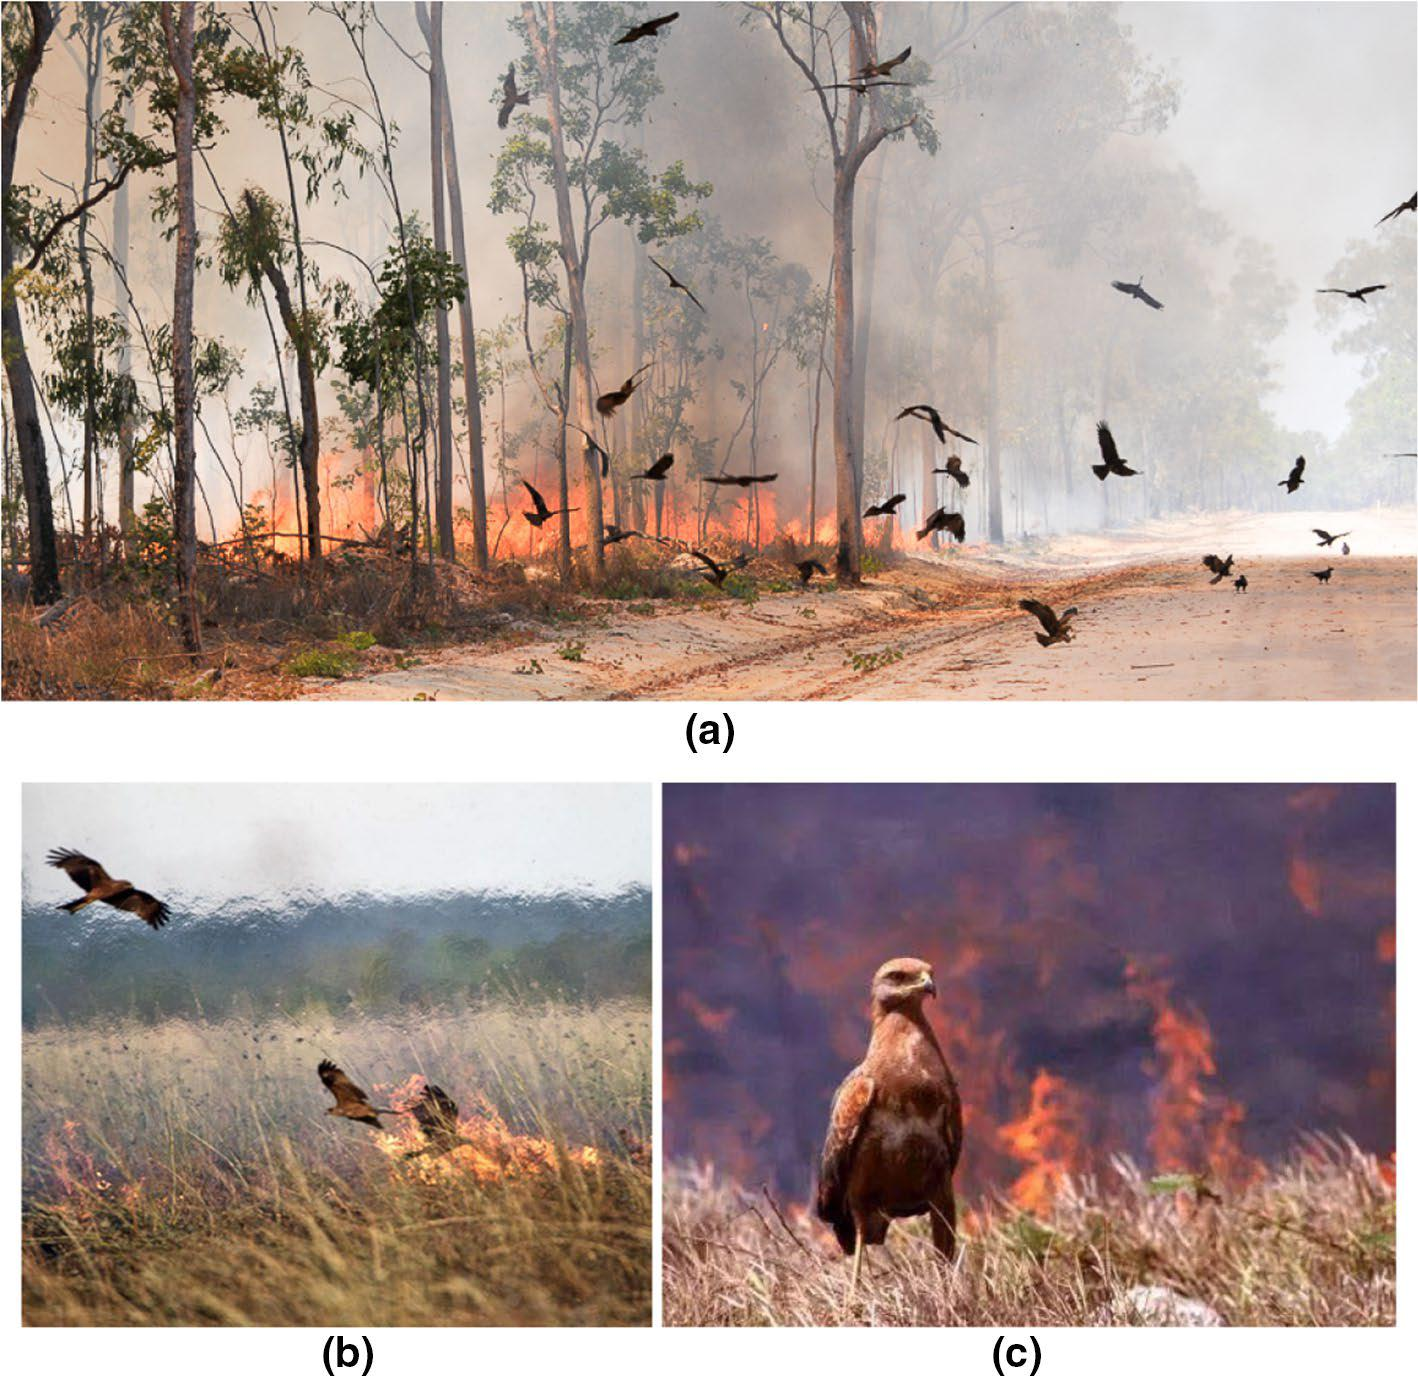
\includegraphics{Gambar FHO/img291.jpg}
\caption{Foto Perilaku Elang Api Terhadap Api (\mycite{azizi2023fire})}
\label{Foto perilaku elang api terhadap api}
\end{figure}

Aktivitas elang ini diilustrasikan pada Gambar \ref{Foto perilaku elang api terhadap api}. Sebagai mekanisme untuk mengendalikan dan menangkap mangsa mereka, burung-burung ini mengambil kayu yang terbakar dan menjatuhkannya di tempat yang tidak terbakar untuk memantik api (a). Api yang terpantik ini akan menakuti mangsa seperti tikus, ular, ataupun hewan lain, dan memaksa mereka mundur (b) ke tempat di mana mereka dapat dimangsa dengan mudah oleh burung-burung elang api ini (c).\\


\indent 
Algoritma\textit{ Fire-Hawk Optimizer} meniru perilaku dari elang api yaitu perilaku mereka mengatur dan menyebarkan api untuk menangkap mangsanya. Lebih rincinya cara kerja algoritma tersebut sebagai berikut. Pertama, ditentukan jumlah kandidat solusi $(X)$ sebagai vektor posisi dari \textit{fire hawk} dan mangsa. Lalu, ditentukan juga inisialisasi secara acak nilai awal vektor posisi di ruang pencarian, yaitu didefinisikan

\begin{align}
    X &= \begin{bmatrix}
    X_1 \\
    X_2 \\
    \vdots \\
    X_i \\
    \vdots \\
    X_N
    \end{bmatrix} 
    = \begin{bmatrix}
    x_1^1 & x_1^2 & \cdots & x_1^a & \cdots & x_1^d \\
    x_2^1 & x_2^2 & \cdots & x_2^a & \cdots & x_2^d \\
    \vdots & \vdots & & \vdots & & \vdots \\
    x_b^1 & x_b^2 & \cdots & x_b^a & \cdots & x_b^d \\
    \vdots & \vdots & & \vdots & & \vdots \\
    x_N^1 & x_N^2 & \cdots & x_N^a & \cdots & x_N^d
    \end{bmatrix},
\end{align}
dan
\begin{align}
    x_i^j(0) &= x_{i,\text{min}}^j + \text{rand}( x_{i,\text{max}}^j - x_{i,\text{min}}^j ), \quad
    i = 1, 2, \ldots, N, \text{ dan } j = 1, 2, \ldots, d.
\end{align}

Notasi $X_i$ merepresentasikan kandidat solusi ke $i$ di ruang pencarian, $d$ merepresentasikan dimensi dari permasalahan, $N$ adalah jumlah total kandidat solusi di ruang pencarian, $x_i^j$ adalah variabel keputusan ke $j$ dari kandidat solusi ke $i$, $x_i^j(0)$ merepresentasikan posisi awal dari kandidat solusi, $x_{i,\text{min}}^j$ dan $x_{i,\text{max}}^j$ adalah batas bawah dan batas atas dari decision variable ke $j$ untuk kandidat solusi ke $i$, dan rand adalah fungsi untuk memilih bilangan acak yang terdistribusi seragam dalam rentang [0,1].\\

Untuk menentukan lokasi \textit{fire hawk} di ruang pencarian, fungsi objektif dievaluasi untuk memilih kandidat solusi dari masalah optimisasi yang dikerjakan. Beberapa kandidat solusi dengan nilai fungsi objektif terbaik direpresentasikan sebagai \textit{fire hawk}, sedangkan kandidat solusi lain dianggap sebagai mangsa. \textit{Fire hawk} yang terpilih dimanfaatkan untuk menyebarkan api di sekitar mangsa di ruang pencarian untuk memudahkan perburuan. Selain itu, solusi global terbaik diasumsikan sebagai api utama yang pertama kali dimanfaatkan oleh \textit{fire hawk} untuk menyebarkan api di ruang pencarian. Skema di atas diilustrasikan pada Gambar \ref{Skema penentuan elang api dan mangsa di ruang pencarian}.

\begin{figure}[H]
    \centering
    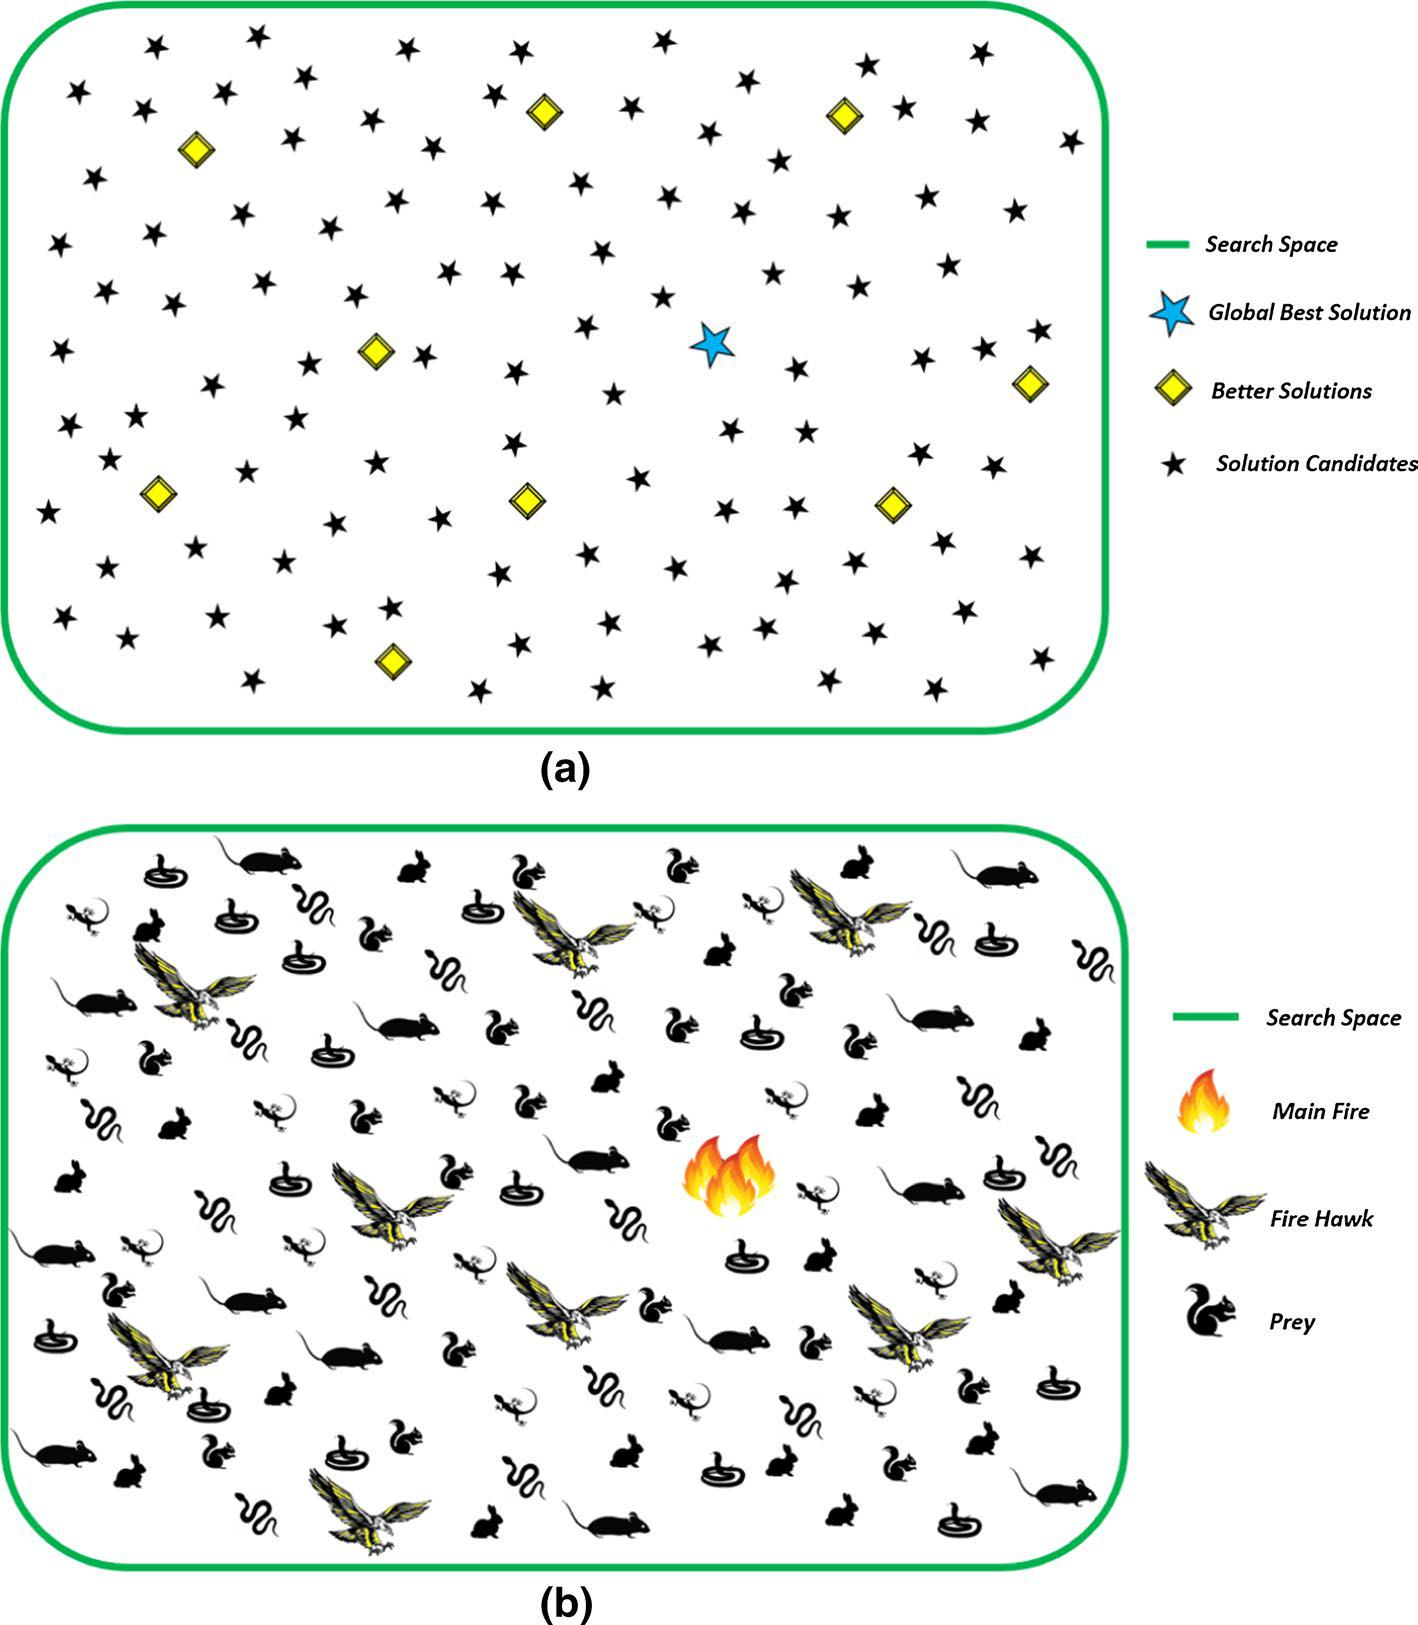
\includegraphics{Gambar FHO/img306.jpg}
    \caption{Skema Penentuan Elang Api dan Mangsa di Ruang Pencarian (\mycite{azizi2023fire})}
    \label{Skema penentuan elang api dan mangsa di ruang pencarian}
\end{figure}

Secara matematis skema tersebut dapat ditulis sebagai

\begin{align}
    PR = \begin{bmatrix}
        PR_1\\
        PR_2\\
        \vdots\\
        PR_k\\
        \vdots\\
        PR_m
    \end{bmatrix},
\end{align}
dan
\begin{align}
    FH = \begin{bmatrix}
        FH_1\\
        FH_2\\
        \vdots\\
        FH_l\\
        \vdots\\
        FH_n
    \end{bmatrix}.
\end{align}

Notasi $PR_k$ adalah mangsa ke-$k$ di ruang pencarian dengan $m$ jumlah keseluruhan mangsa, dan $FH_l$ adalah \textit{fire hawk} ke $l$ dengan $n$ jumlah keseluruhan \textit{fire hawk} di ruang pencarian.\\

Fase berikutnya dari algoritma ini adalah menghitung jumlah jarak antara \textit{fire hawk} dan mangsa, sehingga jarak mangsa terpendek terhadap tiap \textit{fire hawk} dapat ditentukan. Jadi, teritori yang efektif untuk burung-burung ini dapat ditentukan. Dengan kata lain teritori \textit{fire hawk} dengan fungsi objektif terbaik ditentukan dari mangsa-mangsa terdekatnya, teritori \textit{fire hawk} dengan fungsi objektif terbaik kedua ditentukan berdasar mangsa didekatnya yang tidak termasuk dalam teritori \textit{fire hawk} sebelumnya, dan seterusnya. Gambar \ref{Skema perhitungan jarak antara elang api dan mangsa} menunjukkan ilustrasi dari perspektif ini, dengan $D_k^l$ didefinisikan sebagai

\begin{align}
    D_k^l = \sqrt{(x_2-x_1)^2+(y_2-y_1)^2}, \quad
    l = 1, 2, \ldots, n, \text{ dan } k = 1, 2, \ldots, m.
\end{align}

Notasi $D_k^l$ menyatakan jumlah jarak antara \textit{fire hawk} ke-$l$ dan mangsa ke-$k$, $m$ adalah jumlah mangsa di ruang pencarian, $n$ adalah jumlah \textit{fire hawk} di ruang pencarian, dan $(x_1,y_1)$ dan $(x_2,y_2)$ merepresentasikan koordinat dari \textit{fire hawk} di ruang pencarian.\\

\begin{figure}[H]
    \centering
    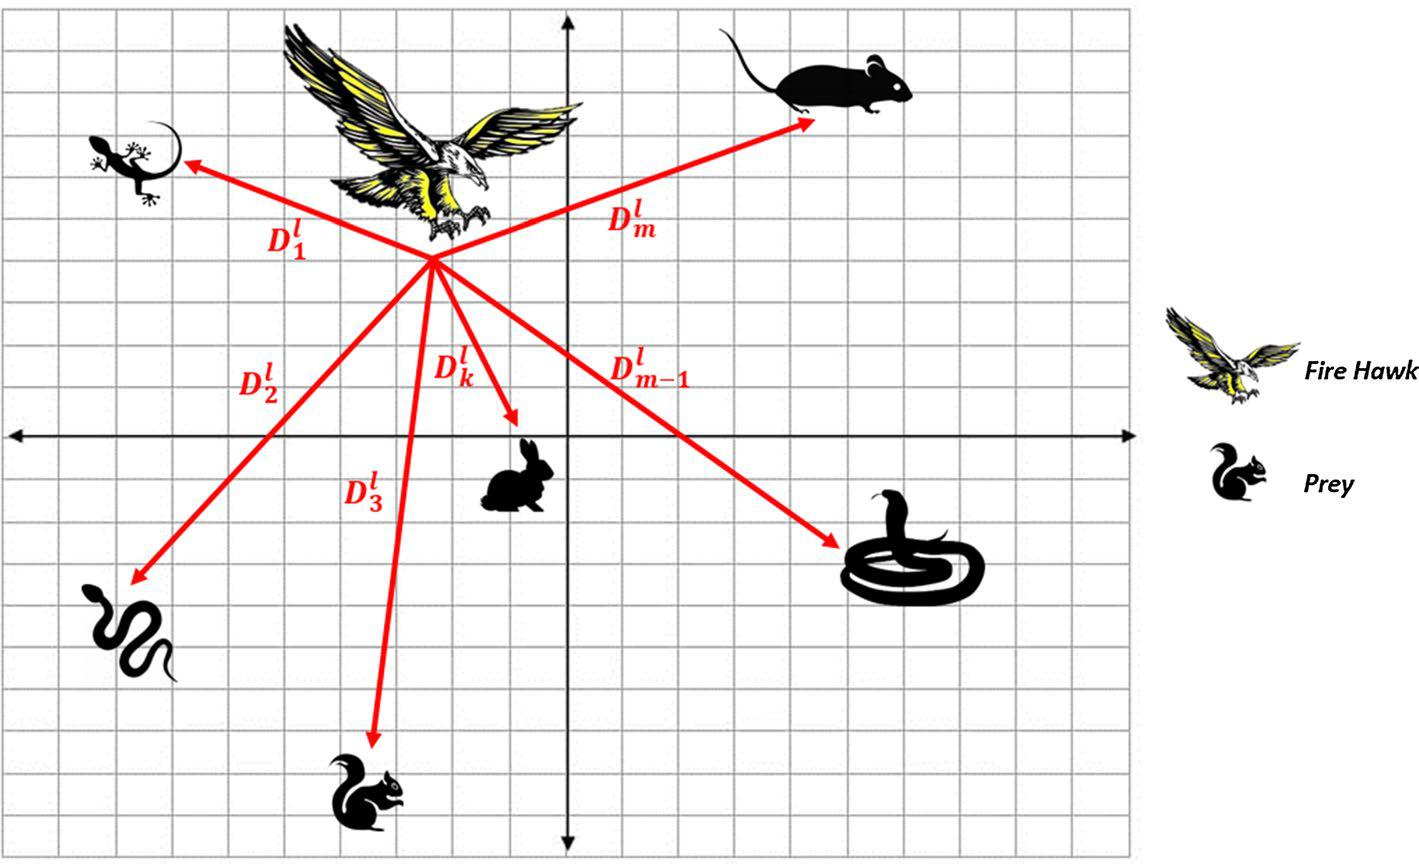
\includegraphics{Gambar FHO/img323.jpg}
    \caption{Skema Perhitungan Jarak Antara Elang Api dan Mangsa (\mycite{azizi2023fire})}
    \label{Skema perhitungan jarak antara elang api dan mangsa}
\end{figure}

Setelah melakukan prosedur yang telah dijelaskan di atas untuk mengukur jarak total antara \textit{fire hawk} dan mangsa, teritori burung-burung ini dapat ditentukan berdasarkan mangsa terdekat di sekitarnya. Dengan mengklasifikasikan \textit{fire hawk} dan mangsa, proses pencarian dari algoritma dapat diatur. Perlu diperhatikan bahwa \textit{fire hawk} dengan nilai fungsi objektif yang lebih baik akan memilih mangsa terdekat terbaik dalam ruang pencarian untuk teritori tertentu. Kemudian, \textit{fire hawk} lain mencari mangsa terdekat lainnya di ruang pencarian, yang menunjukkan bahwa \textit{fire hawk} terkuat melakukan perburuan yang lebih baik daripada \textit{fire hawk} lain. Gambar \ref{Skema penentuan teritori elang api di ruang pencarian} menunjukkan skema penentuan teritori \textit{fire hawk} di ruang pencarian.\\

\begin{figure}[H]
    \centering
    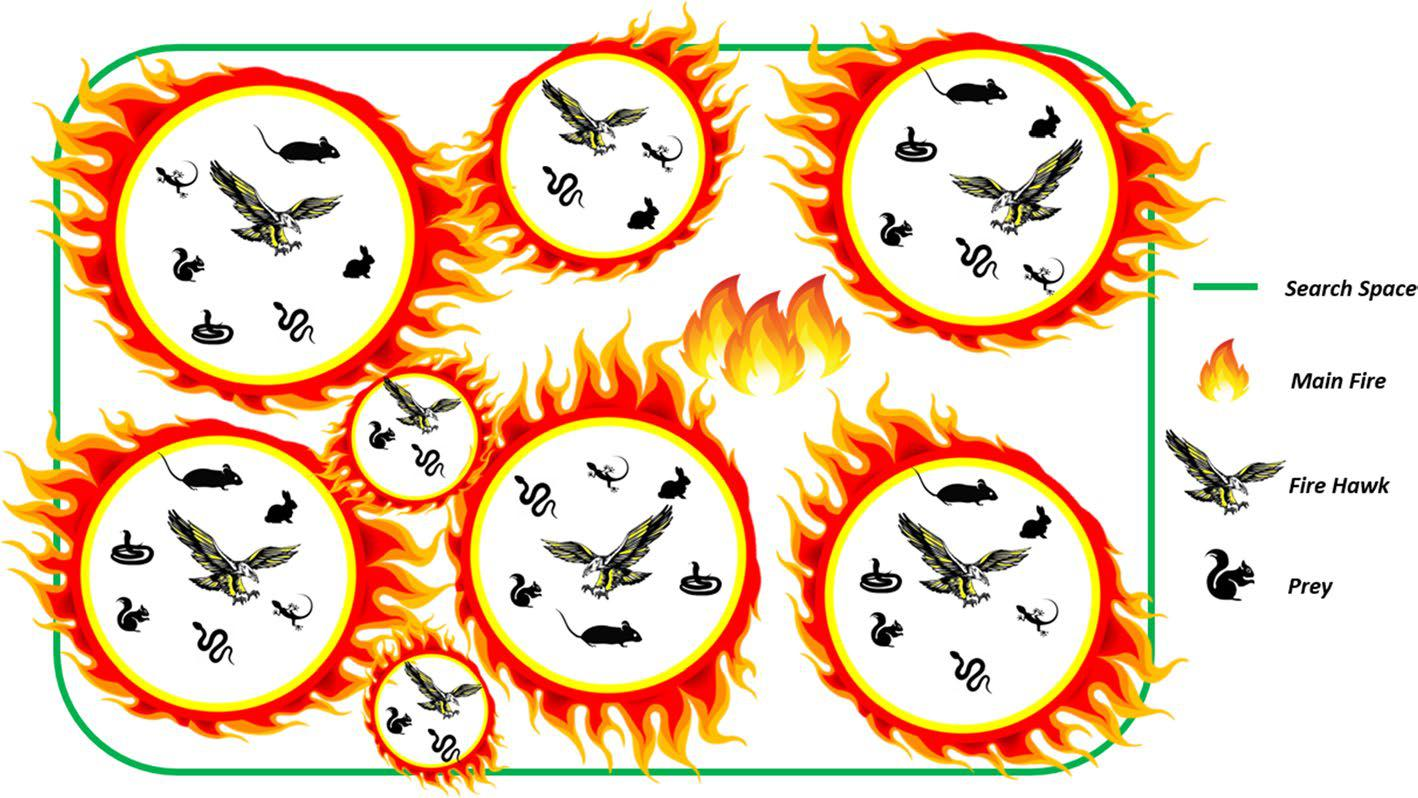
\includegraphics{Gambar FHO/img345.jpg}
    \caption{Skema Penentuan Teritori Elang Api di Ruang Pencarian (\mycite{azizi2023fire})}
    \label{Skema penentuan teritori elang api di ruang pencarian}
\end{figure}

Pada fase berikutnya dari algoritma, \textit{fire hawk} mengumpulkan kayu yang terbakar dari api utama untuk memantik api di area yang dipilih. Pada fase ini, tiap burung membawa kayu yang terbakar lalu menjatuhkannya di teritori tertentu untuk memaksa mangsanya buru-buru melarikan diri. Sedangkan beberapa burung akan menggunakan kayu yang terbakar dari teritori \textit{fire hawk} yang lain sehingga kedua perilaku ini dapat dimanfaatkan untuk memperbarui prosedur dari \textit{loop} pencarian utama FHO, yang ditunjukkan pada persamaan berikut:

\begin{align}
    FH_l^{\textit{new}}=FH_l+(r_1\times GB-r_2\times FH_{\textit{near}}), l=1,2,\ldots,n.
\end{align}

Notasi $FH_l^{\textit{new}}$ menyatakan vektor posisi baru dari \textit{fire hawk} ($FH_l$) ke-$l$, $GB$ adalah solusi global terbaik di ruang pencarian yang dianggap sebagai api utama, $FH_{\textit{near}}$ adalah salah satu \textit{fire hawk} lain di ruang pencarian, dan $r_1$ dan $r_2$ adalah angka acak yang terdistribusi seragam dalam rentang $(0,1)$ untuk menentukan pergerakan dari \textit{fire hawk} terhadap api utama dan teritori \textit{fire hawk} lain. Gambar \ref{Skema proses pembaruan posisi elang api di ruang pencarian} menunjukkan skema pembaruan posisi \textit{fire hawk}.\\

\begin{figure}[H]
    \centering
    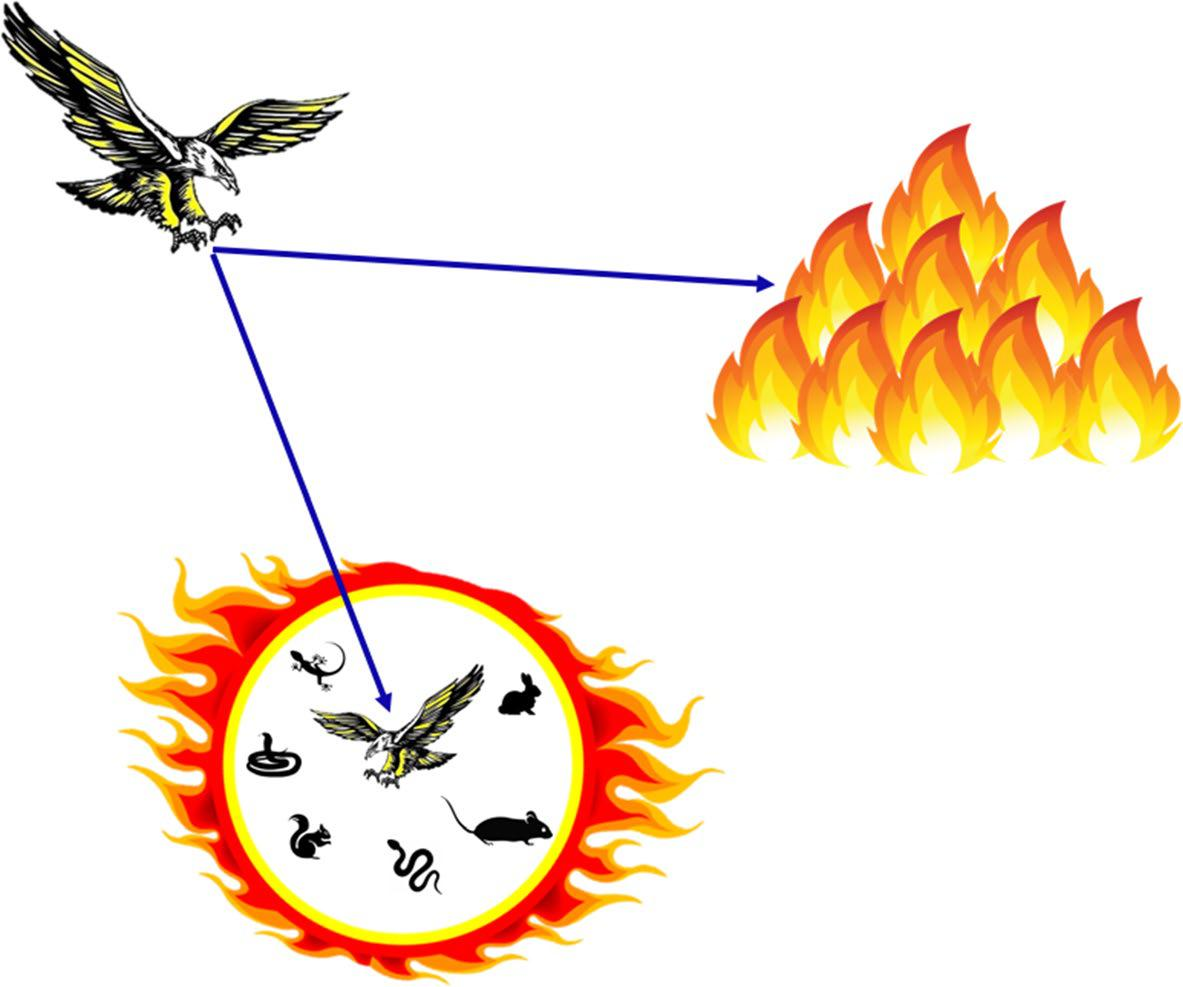
\includegraphics{Gambar FHO/img369.jpg}
    \caption{Skema Proses Pembaruan Posisi Elang Api di Ruang Pencarian (\mycite{azizi2023fire})}
    \label{Skema proses pembaruan posisi elang api di ruang pencarian}
\end{figure}

Fase algoritma selanjutnya, pergerakan dari mangsa di dalam teritori dari tiap \textit{fire hawk} dianggap sebagai kunci dari perilaku hewan untuk proses pembaruan posisi. Ketika kayu yang terbakar dijatuhkan oleh seekor \textit{fire hawk}, mangsa memutuskan untuk bersembunyi, melarikan diri, ataupun berlari ke arah \textit{fire hawk} secara tidak sengaja. Perilaku ini dapat dianggap sebagai proses pembaruan posisi yang dituliskan dengan persamaan berikut:\\

\begin{align}
    PR_q^{\textit{new}}=PR_q+(r_3\times FH_l-r_4\times SP_l), \quad l = 1, 2, \ldots, n, \text{ dan } q = 1, 2, \ldots, r.
\end{align}

\begin{figure}[H]
    \centering
    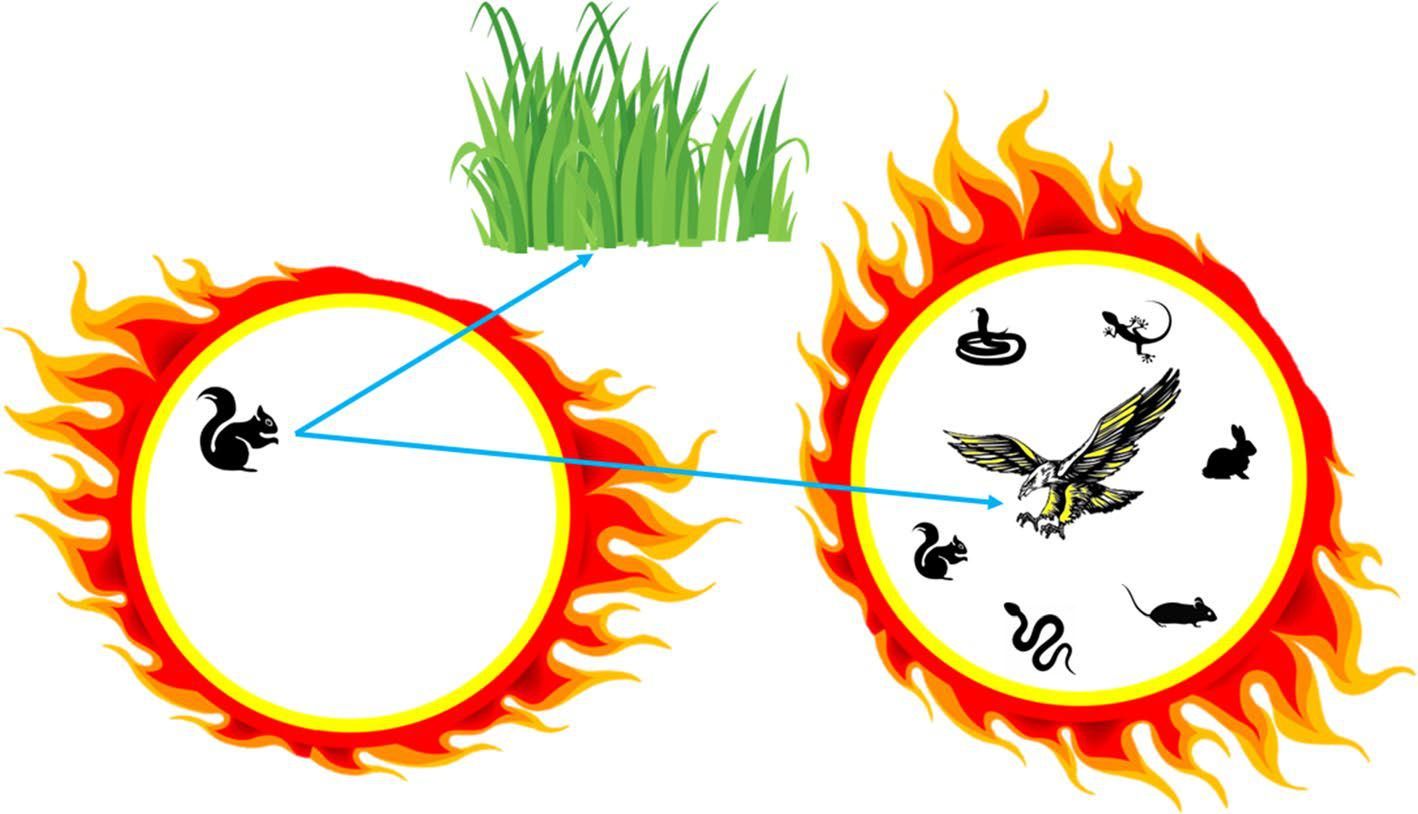
\includegraphics{Gambar FHO/img391.jpg}
    \caption{Skema Proses Pembaruan Posisi Mangsa di Luar Teritori Elang Api (\mycite{azizi2023fire})}
    \label{Skema proses pembaruan posisi mangsa di luar teritori elang api}
\end{figure}

Notasi $PR_q^{\textit{new}}$ menyatakan vektor posisi baru dari mangsa ke-$q$ ($PR_q$) dikelilingi oleh \textit{fire hawk} ke-$l$ ($FH_l$), $GB$ adalah solusi global terbaik di ruang pencarian dianggap sebagai api utama, $SP_l$ adalah tempat aman di dalam teritori \textit{fire hawk} ke-$l$, dan $r_3$ dan $r_4$ adalah bilangan acak yang terdistribusi seragam dalam rentang $(0,1)$ untuk menentukan pergerakan dari mangsa menuju ke \textit{fire hawk} dan tempat aman. Gambar \ref{Skema proses pembaruan posisi mangsa di luar teritori elang api} menunjukkan skema pembaruan posisi mangsa.\\

Selain itu, mangsa melakukan pergerakan menuju teritori \textit{fire hawk} lain ketika ada kemungkinan mangsa akan mendekat ke \textit{fire hawk} di dekat semak-semak atau bahkan bersembunyi di tempat yang lebih aman di luar teritori \textit{fire hawk} yang membuat mereka terjebak. Perilaku ini dapat dianggap sebagai proses pembaruan posisi yang dapat dituliskan dalam persamaan berikut.

\begin{align}
    PR_q^{\textit{new}}=PR_q+(r_5\times FH_{Alter}-r_6\times SP), \quad l = 1, 2, \ldots, n \text{ dan } q = 1, 2, \ldots, r.
\end{align}

Notasi $PR_q^{\textit{new}}$ menyatakan vektor posisi baru dari mangsa ke-$q$ ($PR_q$) dikelilingi oleh \textit{fire hawk} ke-$l$ ($FH_l$), $FH_{Alter}$ adalah salah satu \textit{fire hawk} lain di ruang pencarian, $SP$ adalah tempat aman di luar teritori \textit{fire hawk} ke-$l$, $r_5$ dan $r_6$ adalah bilangan acak yang terdistribusi seragam dalam rentang $(0,1)$ untuk menentukan pergerakan dari mangsa menuju \textit{fire hawk} lain dan tempat aman di luar teritori.\\

Berdasarkan fakta bahwa tempat aman di alam biasanya berupa lokasi di mana sebagian besar hewan berkumpul agar tetap aman dan nyaman selama terdapat ancaman, $SP_l$ dan $SP$ dapat diformulasikan sebagai berikut:

\begin{align}
    \text{SP}_1 &= \frac{\sum_{q=1}^r \text{PR}_q}{r}, \quad q = 1, 2, \ldots, r \text{ dan } l = 1, 2, \ldots, n.\end{align}
\begin{align}
    \text{SP} &= \frac{\sum_{k=1}^m \text{PR}_k}{m}, \quad k = 1, 2, \ldots, m.
\end{align}
    
Notasi $PR_q$ menyatakan mangsa ke-$q$ yang dikelilingi oleh \textit{fire hawk} ke-$l$ ($FH_l$) dan $PR_k$ adalah mangsa ke-$k$ di ruang pencarian.\\

Perlu diperhatikan bahwa teritori dari tiap \textit{fire hawk} diasumsikan sebagai daerah melingkar untuk tujuan visualisasi skema, sehingga definisi dari teritori tergantung jarak secara keseluruhan dari mangsa dan \textit{fire hawk}. Dengan kata lain ketika mangsa diposisikan di teritori \textit{fire hawk} tertentu, diasumsikan mangsa dipengaruhi oleh \textit{fire hawk} tersebut dan bukan yang lain, sehingga jumlah dari mangsa dan jarak mereka terhadap \textit{fire hawk} ditentukan oleh batas dari teritori \textit{fire hawk}. Sedangkan, kemungkinan mangsa berada di luar teritori mereka juga dianggap proses pembaruan posisi terkait fakta bahwa mangsa harus dipengaruhi oleh \textit{fire hawk} dari teritori \textit{fire hawk} lain. Jumlah mangsa tiap \textit{loop} adalah total jumlah kandidat solusi dikurangi dengan jumlah \textit{fire hawk} yang ditentukan secara acak menggunakan \textit{brownian motion} dengan distribusi normal sebagai salah satu distribusi terkenal yang digunakan dalam prosedur pengacakan.\\

Kriteria pemberhentian pada algoritma FHO ini menggunakan kekonvergenan iterasi (\mycite{talbi2009metaheuristics}). Konvergensi terjadi ketika perbaikan solusi antara iterasi berturut-turut menjadi sangat kecil atau tidak signifikan. Lebih rincinya algoritma dihentikan ketika pertidaksamaan berikut dipenuhi, yaitu

\begin{align*}
    \frac{|f(GB_{t+1}-f(GB_T)|}{|f(GB_t)|} < \epsilon.
\end{align*}

 Notasi $f(GB_t)$ menyatakan nilai fungsi objektif dari solusi global terbaik (\textit{Global Best}) pada iterasi ke-$t$, $f(GB_{t+1})$ adalah nilai fungsi objektif dari GB pada iterasi berikutnya, dan $\epsilon$ adalah ambang batas toleransi yang sangat kecil (misalnya, $10^{-6}$). Jika kondisi ini terpenuhi untuk sejumlah iterasi berturut-turut (misalnya, 5 atau 10 iterasi), algoritma dianggap telah konvergen dan dapat dihentikan. Kriteria ini memastikan bahwa algoritma berhenti ketika peningkatan kualitas solusi menjadi minimal yang mengindikasikan bahwa solusi optimal atau mendekati optimal telah ditemukan.

Aspek umum dari FHO termasuk pelanggaran batas dari solusi kandidat di samping kriteria penghentian juga dipertimbangkan dalam model matematika dari algoritma ini. Dalam hal ini, ketentuan matematika juga diimplementasikan dalam algoritma FHO yang mana kontrol batas untuk variabel keputusan yang dilanggar ditentukan, sementara sejumlah evaluasi fungsi objektif atau iterasi yang telah ditentukan sebelumnya atau bahkan kriteria lain seperti kekonvergenan dapat digunakan sebagai kriteria penghentian. Disajikan \textit{pseudo-code} dan \textit{flowchart} dari algoritma FHO di bawah ini.

\begin{algorithm}
\begin{varwidth}{\linewidth}
\caption{Fire Hawk Optimizer (FHO)}
\begin{algorithmic}[1]
\Procedure{Fire Hawk Optimizer}{}
    \State Ditentukan posisi awal dari kandidat solusi $(X_i)$ di raung pencarian dengan $N$ kandidat
    \State Evaluasi nilai \textit{fitness} untuk kandidat solusi awal
    \State Ditentukan solusi global terbaik (GB) sebagai ai utama
    \While{Iterasi $\leq$ iterasi maksimum $\wedge$ konvergensi \textit{counter} $\leq$ iterasi konvergensi maksimum}
        \State Dibentuk $n$ bilangan bulat untuk menentukan jumlah elang api
        \State Ditentukan elang api (FH) dan mangsa-mangsa (PR) di ruang pencarian
        \State Dikalkulasikan total jarak antara elang api dan mangsa-mangsa
        \State Ditentukan teritori elang api dengan menyebarkan mangsa-mangsa
        \For{$l = 1:n$}
            \State Ditentukan posisi baru dari elang api berdasarkan persamaan (3.6)
            \For{$q = 1:r$}
                \State Dikalkulasikan tempat aman di dalam teritori elang api pada persamaan (3.9)
                \State Ditentukan posisi baru dari mangsa-mangsa pada persamaan (3.7)
                \State Dikalkulasikan tempat aman di luar teritori elang api pada persamaan (3.10)
                \State Ditentukan posisi baru dari mangsa-mangsa pada persamaan (3.8)
            \EndFor
        \EndFor
        \State Evaluasi nilai \textit{fitness} untuk elang api dan mangsa-mangsa baru
        \State Ditentukan solusi global terbaik (GB) sebagai api utama
    \EndWhile
    \State \Return GB
\EndProcedure
\end{algorithmic}
\end{varwidth}
\end{algorithm}

Untuk lebih memudahkan penjelasan dari algoritma \textit{Fire Hawk Optimizer} diilustrasikan flowchart algoritma \textit{Fire Hawk Optimizer} pada Gambar \ref{Flowchart FHO} dan Contoh \ref{contoh3.2.1}

\begin{figure}[H]
    \centering
    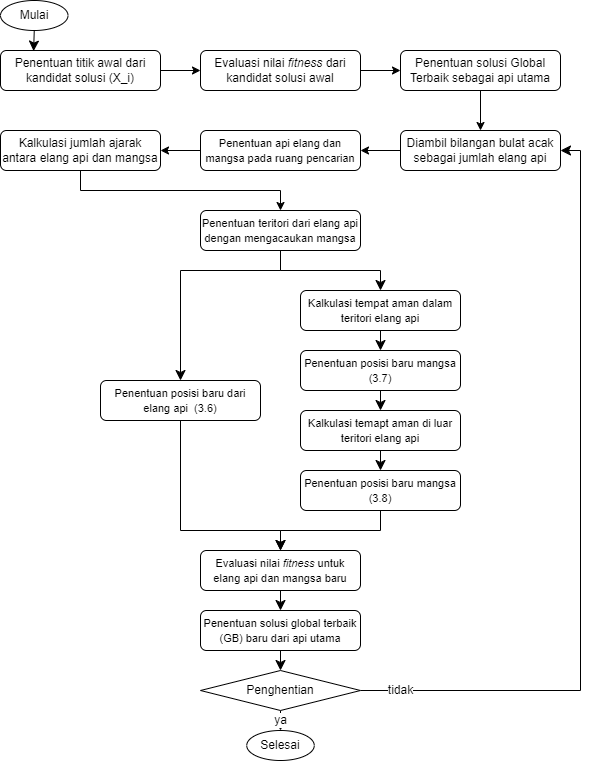
\includegraphics[scale=0.75]{Gambar FHO/FHO.drawio.png}
    \caption{Flowchart FHO}
    \label{Flowchart FHO}
\end{figure}

\begin{contoh}
Akan digunakan algoritma FHO untuk mencari nilai $(x,y)$ yang meminimumkan $f(x,y) = x^2 + y^2$, dengan $-5\leq x \leq 5$ dan $-5\leq y \leq 5$.
\subsection*{1. Inisialisasi}
Misalkan digunakan 5 kandidat solusi di $\R^2$, yaitu 
\begin{align*}
    X &= \begin{bmatrix}
        -2.1 & 3.4 \\
        1.5 & -0.8 \\
        4.2 & 2.7 \\
        -3.6 & -1.9 \\
        0.3 & 4.5
    \end{bmatrix}.
\end{align*}

\subsection*{2. Evaluasi dan Seleksi}
Selanjutnya ditentukan nilai fungsi untuk setiap kandidat sebagai berikut
\begin{align*}
    &f(-2.1, 3.4) = (-2.1)^2 + (3.4)^2 = 4.41 + 11.56 = 15.97, \\
    &f(1.5, -0.8) = (1.5)^2 + (-0.8)^2 = 2.25 + 0.64 = 2.89 ,\\
    &f(4.2, 2.7) = (4.2)^2 + (2.7)^2 = 17.64 + 7.29 = 24.93, \\
    &f(-3.6, -1.9) = (-3.6)^2 + (-1.9)^2 = 12.96 + 3.61 = 16.57, \\
    &f(0.3, 4.5) = (0.3)^2 + (4.5)^2 = 0.09 + 20.25 = 20.34.
\end{align*}

Selanjutnya, dipilih 2 \textit{fire hawk} terbaik kandidat solusi dengan nilai fungsi terendah dan 3 mangsa:
\begin{align*}
    FH &= \begin{bmatrix}
        1.5 & -0.8 \\
        -2.1 & 3.4
    \end{bmatrix}, \\
    PR &= \begin{bmatrix}
        -3.6 & -1.9 \\
        0.3 & 4.5 \\
        4.2 & 2.7
    \end{bmatrix}.
\end{align*}

\subsection*{3. Penentuan teritori}
Berikutnya dihitung jarak antara setiap \textit{fire hawk} dan mangsa.
Untuk $FH_1 = [1.5, -0.8]$, diperoleh
\begin{flushleft}
\begin{align*}
    D_1^1 &= \sqrt{(1.5 - (-3.6))^2 + (-0.8 - (-1.9))^2} = 5.22, \\
    D_2^1 &= \sqrt{(1.5 - 0.3)^2 + (-0.8 - 4.5)^2} = 5.39, \\
    D_3^1 &= \sqrt{(1.5 - 4.2)^2 + (-0.8 - 2.7)^2} = 4.54.
\end{align*}
\end{flushleft}
Untuk $FH_2 = [-2.1, 3.4]$, didapat
\begin{align*}
    D_1^2 &= \sqrt{(-2.1-(-3.6))^2 + (3.4-(-1.9))^2} = 5.59, \\
    D_2^2 &= \sqrt{(-2.1-0.3)^2 + (3.4-4.5)^2} = 2.69, \\
    D_3^2 &= \sqrt{(-2.1-4.2)^2 + (3.4-2.7)^2} = 6.37.
\end{align*}

\subsection*{4. Pembaruan Posisi \textit{Fire hawk}}
Misalkan $r_1 = 0.3$, $r_2 = 0.5$, dan $GB = [1.5, -0.8]$ (\textit{fire hawk} terbaik).
Untuk $FH_1$, didapat
\begin{align*}
    FH_1^{new} &= [1.5, -0.8] + (0.3 \times [1.5, -0.8] - 0.5 \times [-2.1, 3.4]) \\
    &= [1.5, -0.8] + [0.45, -0.24] - [-1.05, 1.7] \\
    &= [3.0, -2.74].
\end{align*}
Untuk $FH_2$, diperoleh
\begin{align*}
    FH_2^{new} &= [-2.1, 3.4] + (0.3 \times [1.5, -0.8] - 0.5 \times [1.5, -0.8]) \\
    &= [-2.1, 3.4] + [0.45, -0.24] - [0.75, -0.4] \\
    &= [-2.4, 3.56].
\end{align*}

\subsection*{5. Pembaruan Posisi Mangsa}
Misalkan $r_3 = 0.4$, $r_4 = 0.6$. Ditentukan tempat aman untuk teritori $FH_1$ (misalkan $PR_1$ dan $PR_3$ ada di teritori ini):
\begin{align*}
    SP_1 &= \frac{[-3.6, -1.9] + [4.2, 2.7]}{2} = [0.3, 0.4]
\end{align*}

Pembaruan posisi $PR_1$:
\begin{align*}
    PR_1^{new} &= [-3.6, -1.9] + (0.4 \times [1.5, -0.8] - 0.6 \times [0.3, 0.4]) \\
    &= [-3.6, -1.9] + [0.6, -0.32] - [0.18, 0.24] \\
    &= [-3.18, -2.46]
\end{align*}

\subsection*{6. Evaluasi dan Iterasi}
Dievaluasi posisi baru dan ulangi proses dari langkah 2 sampai kriteria penghentian terpenuhi (misalnya, jumlah iterasi maksimum atau konvergensi tercapai).

\subsection*{7. Solusi}
Setelah beberapa iterasi, algoritma akan konvergen ke titik (0,0), yang merupakan minimum global dari fungsi $f(x,y) = x^2 + y^2.$
\label{contoh3.2.1}
\end{contoh}

Diselesaikan juga permasalahan sederhana sistem \textit{electric bike-sharing} pada Contoh \ref{contoh3.1.7} menggunakan algoritma \textit{Fire Hawk Optimizer} 

\begin{contoh}
    Akan digunakan permasalahan pada Contoh \ref{contoh3.1.7} dengan menggunakan algoritma \textit{Fire Hawk Optimizer.}

\subsection*{1. Inisialisasi}
Ditentukan jumlah kandidat solusi $(X)$ sebagai vektor posisi dari \textit{fire hawk} dan mangsa, serta ditentukan inisialisasi secara acak sebagai nilai awal vektor posisi di ruang pencarian sebagai berikut,

\begin{align*}
    X &= \begin{bmatrix}
    2 & 1 & 0 & 1 & 0 & 1 & 0 & 0 & 1 & 2 \\
    0 & 3 & 1 & 0 & 0 & 1 & 1 & 0 & 0 & 1 \\
    2 & 1 & 0 & 1 & 1 & 0 & 0 & 1 & 0 & 1 \\
    2 & 1 & 1 & 0 & 0 & 1 & 3 & 0 & 1 & 0 \\
    1 & 2 & 0 & 1 & 0 & 1 & 1 & 1 & 0 & 0 \\
    3 & 0 & 0 & 1 & 0 & 1 & 0 & 0 & 0 & 0 \\
    1 & 2 & 0 & 1 & 0 & 1 & 1 & 0 & 1 & 0 \\
    1 & 2 & 0 & 1 & 1 & 0 & 0 & 1 & 1 & 0 \\
    3 & 0 & 1 & 0 & 1 & 0 & 2 & 0 & 0 & 0 \\
    0 & 3 & 1 & 0 & 1 & 0 & 0 & 1 & 0 & 2
\end{bmatrix}.
\end{align*}
% \begin{align*}
%     x_i^j(0) &= x_{i,\text{min}}^j + \text{rand}( x_{i,\text{max}}^j - x_{i,\text{min}}^j ) \quad \left\{
%     \begin{array}{l}
%     i = 1, 2, \ldots, N \\
%     j = 1, 2, \ldots, d
%     \end{array}
%     \right.
% \end{align*}

\subsection*{2. Evaluasi dan Seleksi}
Fungsi objektif dievaluasi untuk memilih kandidat solusi dari permasalahan. Beberapa kandidat solusi dengan nilai fungsi objektif terbaik direpresentasikan sebagai \textit{fire hawk}, sedangkan kandidat solusi lain dianggap sebagai mangsa. Sehingga didapat \textit{fire hawk} dan mangsa sebagai berikut
\begin{align*}
    FH = \begin{bmatrix}
    3 & 0 & 1 & 0 & 1 & 0 & 2 & 0 & 0 & 0\\
    2 & 1 & 1 & 0 & 0 & 1 & 3 & 0 & 1 & 0    
\end{bmatrix},
\end{align*}
dan
\begin{align*}
    PR = \begin{bmatrix}
    3 & 0 & 0 & 1 & 0 & 1 & 0 & 0 & 0 & 0 \\
    2 & 1 & 0 & 1 & 1 & 0 & 0 & 1 & 0 & 1 \\
    0 & 3 & 1 & 0 & 1 & 0 & 0 & 1 & 0 & 2 \\
    0 & 3 & 1 & 0 & 0 & 1 & 1 & 0 & 0 & 1 \\
    1 & 2 & 0 & 1 & 0 & 1 & 1 & 1 & 0 & 0 \\
    1 & 2 & 0 & 1 & 1 & 0 & 0 & 1 & 1 & 0 \\
    2 & 1 & 0 & 1 & 0 & 1 & 0 & 0 & 1 & 2 \\
    1 & 2 & 0 & 1 & 0 & 1 & 1 & 0 & 1 & 0
\end{bmatrix}.
\end{align*}
Notasi $PR$ menyatakan mangsa di ruang pencarian, dan $FH_l$ adalah \textit{fire hawk} di ruang pencarian.
\subsection*{3. Penentuan teritori}
Selanjutnya, dihitung jumlah jarak antara \textit{fire hawk} dan mangsa untuk menentukan teritori yang efektif. Pada generasi awal ini, terdapat 2 \textit{fire hawk} sehingga dibentuk 2 teritori. Sebagai contoh untuk teritori pertama yaitu teritori elang api dengan nilai fungsi objektif terbaik didapatkan jarak sebagai berikut.
\begin{align*}
    D_1^1 &= 2,8284271247461903,\\
    D_2^1 &= 3,1622776601683795,\\
    D_3^1 &= 3,7416573867739413,\\
    D_4^1 &= 3,7416573867739413,\\
    D_5^1 &= 3,872983346207417,\\
    D_6^1 &= 4,0.
\end{align*}

\subsection*{4. Update Posisi \textit{Fire Hawk}}
Selanjutnya, posisi dari \textit{fire hawk} diperbarui sebagai berikut
\begin{align*}
    FH_l^{\textit{new}}=FH_l+(r_1\times GB-r_2\times FH_{\textit{near}}), l=1,2,\ldots,n.
\end{align*}

Notasi $FH_l^{\textit{new}}$ menyatakan vektor posisi baru dari \textit{fire hawk} ($FH_l$) ke-$l$, $GB$ adalah solusi global terbaik di ruang pencarian yang dianggap sebagai api utama, $FH_{\textit{near}}$ adalah salah satu \textit{fire hawk} lain di ruang pencarian, dan $r_1$ dan $r_2$ adalah bilangan acak yang terdistribusi seragam dalam rentang $(0,1)$.

Misalkan $r_1 = 0.3$, $r_2 = 0.5$, $GB = [3,0,0,1,0,1,0,0,0,0]$, dan $FH_{\textit{near}} = [2,1,1,0,0,1,3,0,1,0]$, maka untuk $FH_1$, didapat
\begin{align*}
    FH_1^{\textit{new}} &= [3,0,1,0,1,0,2,0,0,0] + (0.3 \times [3,0,0,1,0,1,0,0,0,0] \\
    &\indent - 0.5 \times [2,1,1,0,0,1,3,0,1,0])\\
    &= [3,0,1,0,1,0,2,0,0,0] + [0.9,0,0,0.3,0,0.3,0,0,0,0]\\ 
    &\indent - [1,0.5,0.5,0,0,0.5,1.5,0,0.5,0]\\
    &= [2.9,-0.5,0.5,0.3,1,-0.2,0.5,0,-0.5,0]
\end{align*}

\subsection*{5. Tempat Aman dan Update Posisi Mangsa}
Tempat aman dari teritori 1 didapatkan dengan menghitung rata-rata dari semua mangsa di teritori 1 sebagai berikut
\begin{align*}
    SP_1 = \begin{bmatrix}
    1.66666667\\1.33333333\\0.\\1.\\0.33333333\\0.66666667\\0.33333333\\0.5\\0.5\\0.5       
    \end{bmatrix}.
\end{align*}
Ketika kayu yang terbakar dijatuhkan, mangsa memutuskan untuk bersembunyi, melarikan diri, atau berlari ke arah \textit{fire hawk} secara tidak sengaja sehingga terdapat pembaruan posisi mangsa. Sebagai contoh pada mangsa ke 1 jika di dalam teritori didapatkan posisi berikut

\begin{align*}
    PR_1^{\textit{new}} &= PR_1 + (r_3 \times FH_1 - r_4 \times SP_1)
\end{align*}.
Misalkan $r_3 = 0.4$ dan $r_4 = 0.6$, maka didapat
\begin{align*}
    PR_1^{\textit{new}} &= [3,0,0,1,0,1,0,0,0,0] + (0.4 \times [3,0,1,0,1,0,2,0,0,0]\\
    &\indent - 0.6 \times [1.6667,1.3333,0.3333,0.6667,0.6667,0.3333,0,0.6667,0,1])\\
    &= [3,0,0,1,0,1,0,0,0,0] + [1.2,0,0.4,0,0.4,0,0.8,0,0,0] - \\
    &\indent [1,0.8,0.2,0.4,0.4,0.2,0,0.4,0,0.6]\\
    &= [3.2,-0.8,0.2,0.6,0,0.8,0.8,-0.4,0,-0.6]
\end{align*}.

\subsection*{6. Solusi}
Proses di atas dilakukan sebanyak 100 generasi dan didapatkan keputusan terbaik
\begin{align*}
    X = \begin{bmatrix}
    2 & 1 & 1 & 0 & 0 & 1 & 3 & 1 & 1 & 2
    \end{bmatrix},
\end{align*}
yaitu 2 jam operasional untuk sepeda reguler dan 1 jam untuk premium di malam hari. Jika cuaca cerah, operator menambahkan 1 jam operasional untuk sepeda reguler, sehingga jam operasional yang digunakan adalah 3 jam reguler dan 1 jam premium. Jika cuaca hujan, operator menambahkan 1 jam operasional untuk sepeda premium, sehingga jam operasional yang digunakan adalah 2 jam reguler dan 2 jam premium. Strategi ini menghasilkan ekspektasi penggunaan sebesar 3,7 jam per hari.

\end{contoh}
\chapter{SISTEM \textit{ELECTRIC BIKE-SHARING} DI KOTA YOGYAKARTA}

Dalam bab ini akan dibahas pembentukan model sistem \textit{electric bike-sharing} mulai dari asumsi-asumsi, notasi, fungsi tujuan, serta kendala. Permasalahan utama dalam masalah optimalisasi ini yaitu memaksimalkan keuntungan berdasarkan pemilihan stasiun peminjaman, trip yang diterima, dan jumlah sepeda listrik yang perlu dibeli. Permasalahan ini akan dimodelkan menggunakan model \textit{two-stage stochastic} dengan kendala pada tahap pertama terfokus pada perencanaan jangka panjang yaitu lokasi stasiun dan kapasitas sistem (sepeda dan pengisian daya) dan kendala pada tahap kedua berkaitan dengan operasi harian sistem. Model \textit{two-stage stochastic} yang disusun ini akan diselesaikan dengan algoritma \textit{Fire Hawk Optimizer}.

Dalam studi kasus ini, lokasi sistem \textit{electric bike-sharing} yang digunakan dalam simulasi berlokasi di Yogyakarta dengan Tugu Yogyakarta sebagai titik tengah sistem. Selain itu skenario yang digunakan meliputi hari kerja (\textit{weekdays}), Sabtu (\textit{Saturday}), dan Minggu (\textit{Sunday}), dengan probabilitas skenario Minggu yang paling besar, diikuti Sabtu, kemudian hari kerja memiliki probabilitas paling kecil. 

\section{Pemodelan Sistem \textit{Electric Bike-Sharing}}
Sistem \textit{electric bike-sharing} muncul sebagai solusi transportasi perkotaan yang menjanjikan, menawarkan mobilitas yang fleksibel dan ramah lingkungan. Untuk merancang dan mengoperasikan sistem ini secara efisien memerlukan pendekatan canggih untuk mengatasi berbagai tantangan, termasuk ketidakpastian permintaan, manajemen pengisian daya, dan optimalisasi jaringan (\mycitet{brandstatter2017determining}).

\subsection{Kompleksitas Sistem \textit{Electric Bike-Sharing}}
Sistem \textit{electric bike-sharing} memiliki beberapa karakteristik unik yang membuatnya lebih kompleks dibandingkan sistem \textit{bike-sharing} tradisional:
\begin{enumerate}
    \item \textbf{Manajemen Baterai}\\ Sistem menggunakan metode pengisian daya langsung (\textit{direct charging}) yang mana sepeda listrik diisi dayanya saat terparkir di stasiun, bukan menggunakan sistem penukaran baterai (\textit{battery swapping}).
    \item \textbf{Variabilitas Permintaan}\\ Pola permintaan sangat bervariasi tergantung pada waktu, cuaca, dan acara khusus, memerlukan pendekatan yang fleksibel.
    \item \textbf{Optimalisasi Jaringan}\\ Penempatan stasiun yang optimal harus mempertimbangkan tidak hanya aksesibilitas tetapi juga ketersediaan infrastruktur pengisian daya.
    \item \textbf{Keseimbangan Sistem}\\ Menjaga keseimbangan antara ketersediaan sepeda dan slot pengisian di seluruh jaringan merupakan tantangan yang berkelanjutan.
\end{enumerate}

\subsection{Pendekatan Pemodelan Stokastik Dua Tahap}
Untuk mengatasi kompleksitas ini, diadopsi pendekatan pemodelan stokastik dua tahap. Pendekatan ini digunakan karena cocok untuk digunakan dalam pengaplikasian permasalahan transportasi yang melibatkan ketidakpastian.

\begin{enumerate}
    \item \textbf{Tahap Pertama}
    
    Dalam tahap pertama ini keputusan yang diambil  melibatkan perencanaan strategis jangka panjang yaitu terkait lokasi stasiun dan kapasitas sistem.
    \begin{enumerate}
        \item [\textbf{a.}] \textbf{Lokasi Stasiun}\\ Penentuan stasiun pengisian dibangun dengan mempertimbangkan beberapa faktor seperti kepadatan populasi, dan infrastruktur yang ada.
        \item [\textbf{b.}] \textbf{Kapasitas Sistem}\\ Penentuan jumlah sepeda listrik yang akan dibeli dan kapasitas pengisian di setiap stasiun.
    \end{enumerate}
Keputusan ini dibuat sebelum mempertimbangkan permintaan, berdasarkan proyeksi dan analisis skenario. Kemudian setelah ketidakpastian diketahui, dapat ditentukan keputusan pada tahap kedua.

 \item \textbf{Tahap Kedua}
 
    Dalam tahap kedua keputusan yang diambil berkaitan dengan operasi harian sistem.
    \begin{enumerate}
    \item [\textbf{a.}] \textbf{Alokasi Sepeda}\\ Penentuan distribusi sepeda di seluruh jaringan untuk memenuhi permintaan.
    \item [\textbf{b.}] \textbf{Penerimaan Trip}\\ Pengambilan trip mana yang akan diterima berdasarkan ketersediaan sepeda dan status pengisian daya.
    \item [\textbf{c.}] \textbf{Manajemen Pengisian Daya}\\ 
    Manajemen pengisian daya mengikuti beberapa protokol, setiap sepeda yang kembali dari trip langsung masuk ke mode pengisian daya, sepeda dalam status pengisian tidak tersedia untuk trip baru, dan waktu pengisian bergantung pada sisa kapasitas baterai saat kembali.
    \end{enumerate}

Keputusan ini dibuat secara \textit{real-time} atau \textit{near-real-time} setelah permintaan aktual diketahui. Keputusan pada tahap pertama dan tahap kedua diintegrasikan berdasarkan komponen utama model.
\end{enumerate}


\subsection{Komponen Utama Model}
Model yang dikembangkan mengintegrasikan beberapa komponen penting meliputi:
\begin{enumerate}
    \item \textbf{Representasi Jaringan}\\ Dalam hal ini digunakan graf berbobot untuk merepresentasikan jaringan stasiun dan rute perjalanan.
    \item \textbf{Pemodelan Permintaan}\\ Pendekatan berbasis skenario akan diadopsi untuk menangkap variabilitas permintaan.
    \item \textbf{Dinamika Sistem}\\ Graf lokasi \textit{time-expanded} digunakan untuk memodelkan pergerakan sepeda, status pengisian daya, dan alokasi trip dengan setiap titik merepresentasikan kombinasi lokasi stasiun dan waktu diskrit, sementara \textit{arc} menggambarkan aktivitas seperti pengisian daya (\textit{waiting arc}), perjalanan (\textit{travel arc}), serta penempatan awal dan akhir sepeda.
    \item \textbf{Kendala Anggaran dan Operasional}\\ Batasan finansial dan teknis akan dipertimbangkan dalam pengambilan keputusan.
\end{enumerate}

\subsection{Struktur Model}
Model diformulasikan dengan program linear bilangan bulat stokastik, struktur ini dapat mengintegrasikan komponen-komponen di atas untuk masalah optimisasi sistem \textit{electric bike-sharing}.
\begin{enumerate}
    \item \textbf{Fungsi Tujuan}\\ Tujuan adalah memaksimalkan ekspektasi keuntungan, menyeimbangkan pendapatan dari trip yang diterima dengan biaya operasional dan investasi.
    \item \textbf{Kendala Tahap Pertama}\\ Kendala meliputi kendala anggaran, kapasitas sistem, dan lokasi stasiun.
    \item \textbf{Kendala Tahap Kedua}\\ Kendala mencakup keseimbangan alur sepeda bergerak, manajemen pengisian daya, dan pemenuhan permintaan.
    \item \textbf{Variabel Keputusan}\\ Kombinasi variabel biner dan kontinu untuk merepresentasikan keputusan diskrit (seperti pembangunan stasiun) dan kontinu (seperti alokasi sepeda).
\end{enumerate}

\section{Asumsi dan Notasi}

Selanjutnya, dijelaskan mengenai asumsi-asumsi model, yang sebagian besar berdasarkan \mycite{brandstatter2017determining} dengan beberapa modifikasi.
\begin{enumerate}
    \item \textbf{Perkiraan Permintaan}\\ Diasumsikan tersedia perkiraan permintaan pelanggan untuk berbagai skenario (hari kerja) dengan probabilitas terkait. Setiap skenario mencakup set perkiraan trip yang mempertimbangkan aspek spasial dan temporal permintaan.
    \item \textbf{Informasi Trip}\\ Setiap trip memiliki informasi lengkap tentang lokasi asal, tujuan, waktu mulai, dan waktu selesai. Informasi ini memungkinkan estimasi konsumsi baterai dan kontribusi profit untuk setiap trip.
    \item \textbf{Pengisian Daya}\\ Setiap trip yang diterima mengharuskan sepeda listrik memulai perjalanan dalam keadaan baterai terisi penuh. Karakteristik pengisian daya diasumsikan linear terhadap waktu.
    \item \textbf{Kapasitas Stasiun}\\ Setiap lokasi potensial stasiun pengisian memiliki kapasitas maksimum slot pengisian.
    \item \textbf{Jarak Berjalan}\\ Pengguna diasumsikan bersedia berjalan dari/ke stasiun pengisian dalam radius tertentu dari lokasi asal/tujuan mereka.
    \item \textbf{Homogenitas Armada}\\ Operator menggunakan armada sepeda listrik yang homogen untuk mempermudah perencanaan dan perawatan.
    \item \textbf{Fokus Model}\\ Model tidak mempertimbangkan aktivitas operasional staf seperti relokasi sepeda secara manual.
    \item \textbf{Waktu Perjalanan}\\ Waktu perjalanan antara stasiun dianggap deterministik dan konstan.
    \item \textbf{Independensi Skenario}\\ Permintaan dianggap independen antar skenario.
    \item \textbf{Keterbatasan Anggaran}\\ Terdapat batasan anggaran untuk pembangunan stasiun dan pembelian sepeda.
    \item \textbf{Biaya operasional}\\ Terdapat biaya operasional stasiun sejumlah stasiun yang dibangun dan biaya operasional sepeda sejumlah sepeda yang dibeli.
    \item \textbf{Reliabilitas Sepeda}\\ Sepeda diasumsikan selalu dalam kondisi operasional yang baik dan tidak mempertimbangkan kemungkinan kerusakan atau perawatan.
    \item \textbf{Perilaku Pengguna}\\ Pengguna diasumsikan selalu mengembalikan sepeda ke stasiun pengisian dan tidak meninggalkannya di lokasi lain.
    \item \textbf{Kebijakan Harga}\\ Model mengasumsikan kebijakan harga yang tetap dan tidak mempertimbangkan variasi harga berdasarkan waktu atau permintaan.
\end{enumerate}

Asumsi-asumsi ini membantu dalam menyederhanakan kompleksitas sistem \textit{electric bike-sharing}, memungkinkan untuk membangun model matematis yang dapat diselesaikan sambil tetap menangkap esensi dari permasalahan \textit{electric bike-sharing}. Penting untuk dicatat bahwa asumsi-asumsi ini mungkin perlu dimodifikasi atau dilonggarkan, tergantung pada karakteristik spesifik dari sistem yang sedang dimodelkan.

Selanjutnya ditentukan parameter dan variabel yang digunakan berdasarkan asumsi yang telah disebutkan.

\begin{table}[H]
\centering
\begin{tabular}{@{}p{0.2\textwidth}p{0.2\textwidth}p{0.5\textwidth}@{}}
\toprule
Kelompok & Notasi & Deskripsi \\
\midrule
Himpunan dan Indeks & $\Omega$ & Himpunan skenario \\
&$\omega$&Himpunan trip\\
&$K^\omega$ & Himpunan perjalanan dalam skenario $\omega$ \\
& S & Jumlah stasiun potensial\\
& H & Inisial jumlah sepeda yang akan dibeli \\
& T & Periode perencanaan \\
& $i, j \in S$ & Lokasi potensial stasiun \\
& $t \in T$ & Periode waktu, $T = \{0, \ldots, T_{\text{max}}\}$ \\
& $h \in H$ & Himpunan sepeda, $H = \{1, \ldots, H_{\text{max}}\}$ \\
\midrule
Parameter & $\pi_\omega$ & Probabilitas skenario $\omega$ \\
& $p_k$ & Kontribusi keuntungan perjalanan $k$ \\
& $F_i$ & Biaya pembangunan stasiun di lokasi $i$ \\
& $F_{\text{bike}}$ & Biaya pembelian satu sepeda \\
& $\varphi_i$ & Biaya operasional stasiun $i$ \\
& $\phi$ & Biaya operasional per sepeda \\
& $C_i$ & Kapasitas stasiun $i$ \\
& $W$ & Anggaran yang tersedia \\
& $o_k, d_k$ & Asal dan tujuan perjalanan $k$ \\
\midrule
Parameter & $s_k, e_k$ & Waktu mulai dan selesai perjalanan $k$ \\
& $b_k$ & Konsumsi baterai perjalanan $k$ \\
& $\rho$ & Laju pengisian daya per unit waktu \\
& $r$ & Jarak maksimum yang diizinkan antar stasiun \\
\bottomrule
\end{tabular}
\end{table}

\begin{table}[H]
\centering
\begin{tabular}{@{}p{0.2\textwidth}p{0.2\textwidth}p{0.5\textwidth}@{}}
\toprule
Kelompok & Notasi & Deskripsi \\
\midrule
Variabel Tahap Pertama & $y_i $ & $
y_i = 
\begin{cases} 
1, & \text{jika stasiun } i \text{ dibangun} \\
0, & \text{jika stasiun } i \text{ tidak dibangun}
\end{cases}
$, $y_i \in \{0,1\}, i \in S $ \\
& $z_h$ & $
z_h = 
\begin{cases} 
1, & \text{jika sepeda } h \text{ dibeli} \\
0, & \text{jika sepeda } h \text{ tidak dibeli}
\end{cases}
$, $z_h \in \{0,1\}, h \in H $ \\
\midrule
Variabel Tahap Kedua & $x_k^\omega$ & Apakah perjalanan $k$ diterima dalam skenario $\omega$ \\
& $x_k^{h,\omega}$ & Apakah perjalanan $k$ ditugaskan ke sepeda $h$ dalam skenario $\omega$ \\
& $f_a^{h,\omega}$ & Apakah sepeda $h$ melintasi \textit{arc} $a$ dalam skenario $\omega$ \\
\midrule
Graf dengan ekspansi waktu & $G^\omega = (V^\omega, A^\omega)$ & Graf lokasi dengan ekspansi waktu dalam skenario $\omega$ \\
& $A_I^\omega$ & Himpunan \textit{arc} alokasi awal dalam skenario $\omega$ \\
& $A_W^\omega$ & Himpunan \textit{arc} tunggu dalam skenario $\omega$ \\
& $A_C^\omega$ & Himpunan \textit{arc} pengumpulan akhir dalam skenario $\omega$ \\
& $A_T^\omega$ & Himpunan \textit{arc} perjalanan dalam skenario $\omega$ \\
& $r^\omega$ & Titik akar dalam skenario $\omega$ \\
& $s^\omega$ & Titik tujuan dalam skenario $\omega$ \\
\bottomrule
\end{tabular}
\end{table}

\section{Formulasi Permasalahan}

Dalam subbab ini akan diformulasikan masalah program linear bilangan bulat stokastik dua tahap sistem \textit{electric bike-sharing}

\begin{enumerate}
    \item Fungsi Objektif
    
    Berdasarkan struktur model yang telah dipaparkan, dibentuk fungsi tujuan dengan memaksimalkan keuntungan yang diharapkan dengan menyeimbangkan pendapatan dari trip yang diterima dengan biaya operasional dan investasi. Fungsi objektif dari model ini memaksimalkan ekspektasi profit, yaitu 
    
    \begin{equation}
        \max \sum_{\omega \in \Omega} \pi_{\omega} \left( \sum_{k \in K_{\omega}} p_k x_k^\omega \right) - \sum_{i \in S} \varphi_i y_i - \sum_{h \in H} \phi z_h.
        \label{Fungsi objektif}
    \end{equation}
    
    Fungsi objektif \eqref{Fungsi objektif} terbagi menjadi 3 bagian yaitu:
    \begin{enumerate}
        \item [a.] Ekspektasi pendapatan: $\sum_{\omega \in \Omega} \pi_{\omega} \left( \sum_{k \in K_{\omega}} p_k x_k^\omega \right)$ jumlahan ini merupakan jumlahan dari keuntungan $p_k$ dari setiap trip $x_k$ dengan pembobotan probabilitas skenario $\pi_\omega$.
        \item [b.] Biaya operasional stasiun: $\sum_{i \in S} \varphi_i y_i$ jumlahan ini merupakan jumlahan dari biaya operasi $\varphi_i$ untuk setiap stasiun $y_i$ yang dibangun.
        \item [c.] Biaya operasional sepeda: $\sum_{h \in H} \phi z_h$ jumlahan ini merupakan jumlahan biaya operasi $\phi$ dari setiap sepeda yang dibeli $z_h$.
    \end{enumerate}
    
    \item Kendala Tahap Pertama
    \begin{enumerate}
        \item [a.] Kendala anggaran:
        \begin{equation}
        \sum_{i \in S} F_i y_i + \sum_{h \in H} F_{\text{bike}} z_h \leq W,
        \end{equation}
        Kendala ini memastikan total biaya pembangunan stasiun ($F_i y_i$) dan pembelian sepeda ($F_{\text{bike}} z_h$) tidak melebihi anggaran yang tersedia $W$.\\
        \item [b.] Kendala radius pembangunan stasiun:
        \begin{equation}
        y_i + y_j \leq 1 \quad \forall i, j \in S, \; i < j, \; d(i, j) \leq r.
        \end{equation}
        Kendala ini memastikan bahwa jika dua lokasi stasiun potensial $i$ dan $j$ memiliki jarak kurang dari atau sama dengan radius minimum $r$, maka paling banyak hanya satu stasiun yang dapat dibangun di antara keduanya.\\
        \end{enumerate}
    
    
    \item Kendala Tahap Kedua
    \begin{enumerate}
        \item [a.]  Kendala penerimaan trip:
    \begin{equation}
    \sum_{h \in H} x_k^{h,\omega} = x_k^\omega \quad \forall \omega \in \Omega, k \in K_\omega,
    \end{equation}
    kendala ini memastikan jika trip $k$ diterima di skenario $\omega$ ($x_k^\omega = 1$), harus ditetapkan untuk satu sepeda saja.\\
        \item [b.] Kendala alokasi sepeda:
    \begin{equation}
    x_k^{h,\omega} \leq z_h \quad \forall h \in H, \forall \omega \in \Omega, \forall k \in K_\omega,
    \end{equation}
    kendala ini memastikan trip hanya bisa ditetapkan ke sepeda jika sepeda tersebut telah dibeli ($z_h = 1$).\\
        \item [c.] Kendala kapasitas stasiun:
    \begin{equation}
    \sum_{h \in H} \sum_{a \in \delta^+(i_t) \cap (A_W^\omega \cup A_C^\omega)} f_a^{h,\omega} \leq C_i y_i \quad \forall \omega \in \Omega, \forall i_t \in V^\omega \setminus \{r^\omega, s^\omega\},
    \end{equation}
    Kendala ini memastikan jumlah sepeda pada sebuah stasiun (entah dalam waktu tunggu atau sudah terparkir) tidak boleh melebihi kapasitas stasiun $C_i$ jika stasiun dibangun ($y_i = 1$).\\
        \item [d.] Kendala konservasi arus:
    \begin{equation}
    f^{h,\omega}[\delta^-(i_t)] = f^{h,\omega}[\delta^+(i_t)] \quad \forall h \in H, \forall \omega \in \Omega, \forall i_t \in V^\omega \setminus \{r^\omega, s^\omega\},
    \end{equation}
    Kendala ini memastikan jumlah sepeda yang memasuki  node (stasiun dalam waktu tertentu) harus sama dengan jumlah stasiun yang meninggalkan node tersebut, untuk mempertahankan konservasi aliran.\\
        \item [e.] Kendala alokasi awal:
    \begin{equation}
    f^{h,\omega}[A_I^\omega] = z_h \quad \forall h \in H, \forall \omega \in \Omega,
    \end{equation}
    Kendala ini memastikan tiap sepeda yang dibeli ($z_h = 1$) dialokasikan di stasiun awal dari skenario.\\
    \item [f.] Kendala waktu pengisian daya:
    \begin{equation}
    \begin{aligned}
    f_a^{h,\omega} \leq f_{a'}^{h,\omega} \quad & \forall h \in H, \forall \omega \in \Omega, \forall k \in K^\omega, \forall a = (i_{s_k}, j_{e_k}) \in A_T^\omega(k), \\
    & \forall a' = (j_t, j_{t'}) \in A_W^\omega, t \geq e_k, t' \leq e_k + \left\lceil \frac{b_k}{\rho} \right\rceil,
    \end{aligned}
    \end{equation}
    Kendala ini memastikan setelah trip, sepeda tetap pada stasiun untuk pengisian daya. Kendala ini memaksa sepeda untuk tetap di stasiun akhir untuk waktu yang diperlukan untuk pengisian ulang daya baterau yang telah terpakai pada trip ($\left\lceil \frac{b_k}{\rho} \right\rceil$).\\ 
    \end{enumerate}
   
    
    
    
    
    \item Domain variabel
    \begin{align}
    y_i &\in \{0, 1\} \quad \forall i \in S, \\
    z_h &\in \{0, 1\} \quad \forall h \in H, \\
    x_k^\omega &\in \{0, 1\} \quad \forall k \in K^\omega, \forall \omega \in \Omega, \\
    x_k^{h,\omega} &\in \{0, 1\} \quad \forall h \in H, \forall \omega \in \Omega, \forall k \in K^\omega, \\
    f_a^{h,\omega} &\in \{0, 1\} \quad \forall h \in H, \forall \omega \in \Omega, \forall a \in A^\omega.
    \end{align}
    Kendala-kendala ini mendefinisikan semua variabel keputusan dalam bentuk biner ($\{0, 1\}$), yang menunjukkan bahwa stasiun dibangun atau tidak, sepeda dibeli atau tidak, trip diterima atau tidak, trip ditetapkan pada sepeda tertentu atau tidak, dan kendala operasional seperti waktu pengisian daya dan kapasitas stasiun.
    \end{enumerate}




Berdasarkan konstruksi di atas, permasalahan SCSLP dapat dituliskan sebagai berikut:
\begin{align}
    \max \sum_{\omega \in \Omega} \pi_{\omega} \left( \sum_{k \in K_{\omega}} p_k x_k^\omega \right) - \sum_{i \in S} F_i y_i - \sum_{h \in H} F_{\text{bike}} z_h.
\end{align}
dengan kendala:
\textbf{First-stage}
\begin{align}
    \sum_{i \in S} F_i y_i + \sum_{h \in H} F_{\text{bike}} z_h \leq W,\\
    y_i + y_j \leq 1 \quad \forall i, j \in S, \; i < j, \; d(i, j) \leq r.
\end{align}
\textbf{Second-stage}:
\begin{align}
    &\sum_{h \in H} x_k^{h,\omega} = x_k^\omega \quad \forall \omega \in \Omega, k \in K_\omega,\\
    &x_k^{h,\omega} \leq z_h \quad \forall h \in H, \forall \omega \in \Omega, \forall k \in K_\omega,\\
    &\sum_{h \in H} \sum_{a \in \delta^+(i_t) \cap (A_W^\omega \cup A_C^\omega)} f_a^{h,\omega} \leq C_i y_i \quad \forall \omega \in \Omega, \forall i_t \in V^\omega \setminus \{r^\omega, s^\omega\},\\
    &f^{h,\omega}[\delta^-(i_t)] = f^{h,\omega}[\delta^+(i_t)] \quad \forall h \in H, \forall \omega \in \Omega, \forall i_t \in V^\omega \setminus \{r^\omega, s^\omega\},\\
    &f^{h,\omega}[A_I^\omega] = z_h \quad \forall h \in H, \forall \omega \in \Omega,\\
    \begin{split}
        f_a^{h,\omega} \leq f_{a'}^{h,\omega} \quad \forall h \in H, \forall \omega \in \Omega, \forall k \in K^\omega, \forall a = (i_{s_k}, j_{e_k}) \in A_T^\omega(k), \\
        \forall a' = (j_t, j_{t'}) \in A_W^\omega, t \geq e_k, t' \leq e_k + \left\lceil \frac{b_k}{\rho} \right\rceil.
    \end{split}
\end{align}
\textbf{Domain Variabel}:
\begin{align}
y_i &\in \{0, 1\} \quad \forall i \in S, \\
z_h &\in \{0, 1\} \quad \forall h \in H, \\
x_k^\omega &\in \{0, 1\} \quad \forall k \in K^\omega, \forall \omega \in \Omega, \\
x_k^{h,\omega} &\in \{0, 1\} \quad \forall h \in H, \forall \omega \in \Omega, \forall k \in K^\omega, \\
f_a^{h,\omega} &\in \{0, 1\} \quad \forall h \in H, \forall \omega \in \Omega, \forall a \in A^\omega.
\end{align}

\section{Simulasi}

Selanjutnya akan dibahas penyelesaian masalah \textit{two-stage stochastic} untuk memaksimalkan profit dari sistem \textit{bike-sharing} berbasis stasiun. Masalah optimisasi ini melibatkan lokasi serta biaya pembangunan stasiun yang optimal, trip yang diterima beserta profit kontribusi tiap tripnya, dan juga jumlah dan harga sepeda yang akan dibeli. Penyelesaian model ini akan menggunakan algoritma metaheuristik yaitu \textit{Fire Hawk Optimizer}.

Selanjutnya wilayah yang digunakan dalam simulasi berlokasi di Yogyakarta dengan pusat lokasi berada di Tugu Yogyakarta. Lokasi potensial untuk pembangunan stasiun dan juga trip-trip tiap skenario di-\textit{generate} secara acak. Kemudian, biaya pembangunan stasiun, profit kontribusi, dan juga harga sepeda tidak menggunakan mata uang khusus tapi di-\textit{generate} semasuk akal mungkin seperti harga sepeda dan pembangunan stasiun yang terlampau tinggi selisihnya.

\subsection{Generating Data}
Untuk mensimulasikan sistem \textit{electric bike-sharing} di Yogyakarta, digunakan data yang dihasilkan secara acak dengan beberapa parameter dan batasan yang realistis. Berikut adalah rincian data yang dihasilkan.

\begin{enumerate}
    \item \textbf{Lokasi Stasiun}\\ Dalam kasus ini diambil 15 titik potensial untuk pembangunan stasiun pengisian daya $(i)$. Lokasi ini mencakup beberapa tempat strategis di Yogyakarta, termasuk Stasiun Tugu, Malioboro Mall, Pasar Beringharjo, Bank Indonesia Yogyakarta, Keraton Yogyakarta, dan Universitas Gadjah Mada, serta beberapa lokasi acak lainnya.
    \item \textbf{Kapasitas Stasiun}\\ Setiap stasiun potensial memiliki kapasitas $(C_i)$ yang bervariasi antara 5 hingga 10 slot sepeda.
    \item \textbf{Skenario}\\ Dalam kasus ini dibuat 3 skenario $(\Omega)$ berdasarkan hari (Senin-Jumat) yaitu hari kerja, Sabtu, dan Minggu dengan masing-masing skenario memiliki probabilitas ($\pi_{\omega}$) yaitu $0.30, 0.34, \text{dan } 0.36$ untuk mensimulasikan variasi permintaan. 
    \item \textbf{Trip}\\ Setiap skenario memiliki 30 trip $(K^\omega)$ yang dibangkitkan secara acak dengan mempertimbangkan lokasi stasiun, jarak maksimum baterai, dan waktu perjalanan.
    \item \textbf{Waktu Perencanaan}\\ Periode perencanaan $(T_{max})$ ditetapkan selama 15 unit waktu.
    \item \textbf{Anggaran}\\ Anggaran total $(W)$ ditetapkan sebesar 1.200.000.000.
    \item \textbf{Biaya Pembukaan Stasiun}\\ Biaya pembukaan stasiun $(F_i)$ dihitung berdasarkan komponen tetap $(\alpha)$ antara 10.000.000 hingga 50.000.000, dan komponen variabel $(\beta)$ antara 2.000.000 hingga 5.000.000 per kapasitas.
    \item \textbf{Sepeda Listrik}\\ Jumlah maksimum sepeda listrik yang dapat dibeli tidak ditentukan secara eksplisit, tetapi dibatasi oleh anggaran dan kapasitas stasiun.
    \item \textbf{Biaya Operasional}\\ Biaya operasional per sepeda $(\phi)$ dan per stasiun $(\varphi_i)$ tidak ditentukan secara eksplisit dalam data yang dihasilkan.
    \item \textbf{Profit}\\ Profit per trip dihitung berdasarkan durasi perjalanan, dengan rate 10.000.000 per unit waktu.
    \item \textbf{Konsumsi Baterai}\\ Konsumsi baterai untuk setiap trip dihitung berdasarkan jarak perjalanan relatif terhadap jarak maksimum baterai (50 km).
\end{enumerate}
Data ini digunakan untuk membuat peta interaktif yang menunjukkan lokasi potensial stasiun dan trip yang mungkin terjadi. Peta ini disimpan sebagai file HTML untuk visualisasi lebih lanjut.

\begin{figure}[H]
    \centering
    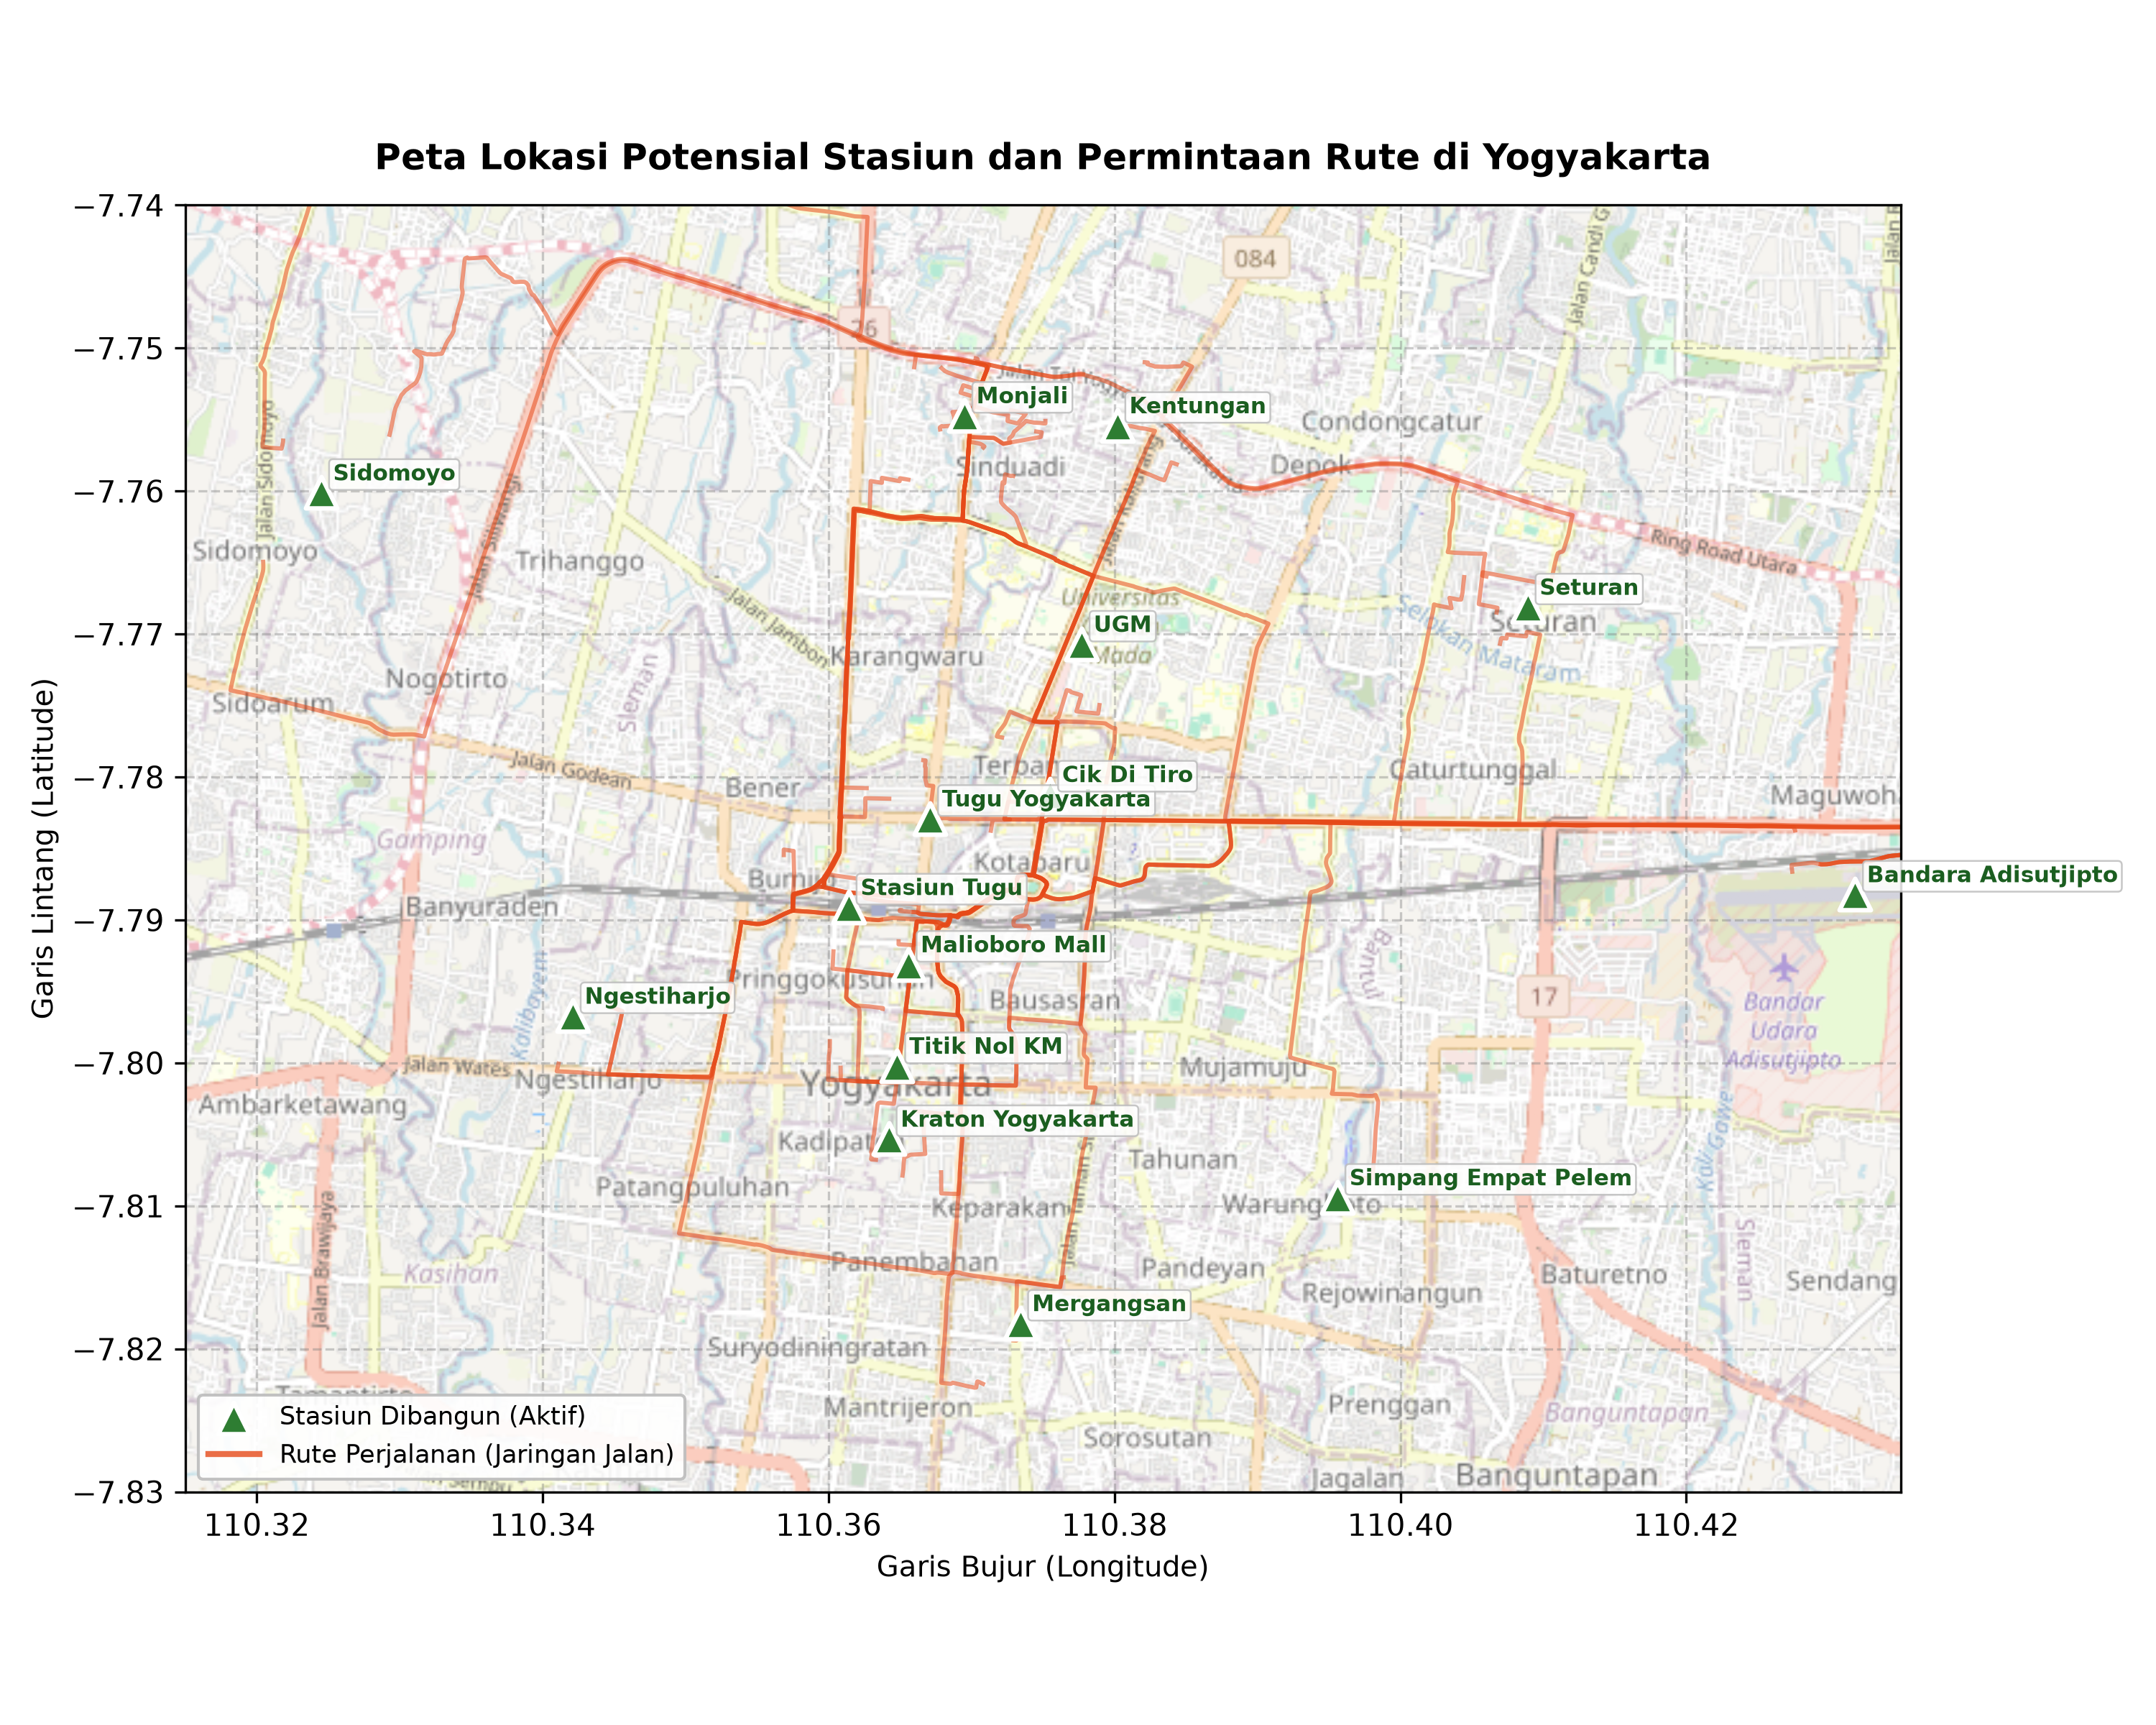
\includegraphics[scale=0.8]{Inisial.png}
    \caption{Peta Lokasi Potensial Pembangunan Stasiun}
    \label{Peta lokasi potensial pembangunan stasiun}
\end{figure}

\section{Prosedur Algoritma \textit{Fire Hawk Optimizer}}


Algoritma \textit{Fire Hawk Optimizer} (FHO) diaplikasikan untuk menyelesaikan permasalahan optimisasi lokasi stasiun pengisian daya dalam sistem \textit{electric bike-sharing}. Berikut adalah langkah-langkah utama dari algoritma FHO:

\subsection{Inisialisasi}

Langkah pertama dilakukan dengan menentukan jumlah kandidat solusi $(X)$ sebagai vektor posisi dari elang api dan mangsa. Setiap kandidat solusi merepresentasikan konfigurasi potensial dari sistem \textit{electric bike-sharing}, termasuk lokasi stasiun pengisian daya, alokasi sepeda listrik, dan trip yang diterima. Nilai awal ditentukan secara acak dalam batas-batas yang ditentukan oleh kendala sistem, seperti anggaran dan kapasitas maksimum stasiun.

\begin{align}
    X &= \begin{bmatrix}
    X_1 \\
    X_2 \\
    \vdots \\
    X_i \\
    \vdots \\
    X_N
    \end{bmatrix} 
    = \begin{bmatrix}
    x_1^1 & x_1^2 & \cdots & x_1^a & \cdots & x_1^d \\
    x_2^1 & x_2^2 & \cdots & x_2^a & \cdots & x_2^d \\
    \vdots & \vdots & & \vdots & & \vdots \\
    x_b^1 & x_b^2 & \cdots & x_b^a & \cdots & x_b^d \\
    \vdots & \vdots & & \vdots & & \vdots \\
    x_N^1 & x_N^2 & \cdots & x_N^a & \cdots & x_N^d
    \end{bmatrix},
\end{align}
dan
\begin{align}
    x_i^j(0) &= x_{i,\text{min}}^j + \text{rand}( x_{i,\text{max}}^j - x_{i,\text{min}}^j ), \quad i = 1, 2, \ldots, N, \text{ dan } j = 1, 2, \ldots, d,
\end{align}

dengan
\begin{enumerate}
    \item $X_i$ merepresentasikan kandidat solusi ke $i$ di ruang pencarian,
    \item $d$ merepresentasikan dimensi dari permasalahan (misalnya, jumlah lokasi potensial stasiun plus jumlah sepeda yang dapat dialokasikan),
    \item $N$ adalah jumlah total kandidat solusi di ruang pencarian,
    \item $x_i^j$ adalah variabel keputusan ke $j$ dari kandidat solusi ke $i$ (misalnya, keputusan untuk membangun stasiun di lokasi tertentu atau jumlah sepeda yang dialokasikan),
    \item $x_i^j(0)$ merepresentasikan posisi awal dari kandidat solusi,
    \item $x_{i,\text{min}}^j$ dan $x_{i,\text{max}}^j$ adalah batas bawah dan batas atas dari variabel keputusan ke $j$ untuk kandidat solusi ke $i$,
    \item rand adalah bilangan acak yang terdistribusi seragam dalam rentang [0,1], dan
    \item $i = 1, 2, \ldots, N$ dan $j = 1, 2, \ldots, d$.
\end{enumerate}

\subsection{Evaluasi dan Seleksi}
Fungsi objektif ini merepresentasikan total profit yang diharapkan dari operasi sistem \textit{electric bike-sharing}, dengan mempertimbangkan pendapatan dari perjalanan yang diterima, biaya pembangunan stasiun, dan biaya operasional.\\

Beberapa kandidat solusi dengan nilai fungsi objektif terbaik direpresentasikan sebagai elang api, sedangkan kandidat solusi lain dianggap sebagai mangsa. Elang api yang dipilih dimanfaatkan untuk menyebarkan api di sekitar mangsa di ruang pencarian untuk memudahkan perburuan. Hal ini dapat diinterpretasikan sebagai eksplorasi area di sekitar solusi-solusi terbaik untuk menemukan konfigurasi sistem \textit{electric bike-sharing} yang lebih optimal.\\

Solusi terbaik global diasumsikan sebagai api utama yang pertama kali dimanfaatkan oleh elang api untuk menyebarkan api di ruang pencarian. Ini merepresentasikan konfigurasi terbaik sistem \textit{electric bike-sharing} yang ditemukan sejauh ini. Solusi-solusi yang direpresentasikan sebagai elang api dan mangsa dinyatakan sebagai berikut.
\begin{align}
    PR = \begin{bmatrix}
        PR_1\\
        PR_2\\
        \vdots\\
        PR_k\\
        \vdots\\
        PR_m
    \end{bmatrix},
\end{align}

dan

\begin{align}
    FH = \begin{bmatrix}
        FH_1\\
        FH_2\\
        \vdots\\
        FH_l\\
        \vdots\\
        FH_n
    \end{bmatrix},
\end{align}
dengan
\begin{enumerate}
    \item notasi $PR_k$ adalah mangsa ke-$k$ di ruang pencarian berdasarkan jumlah angka dari mangsa $m$. Mangsa-mangsa ini merepresentasikan solusi-solusi yang kurang optimal untuk sistem \textit{electric bike-sharing},
    \item notasi $FH_l$ adalah elang api ke $l$ berdasarkan jumlah dari $n$ elang api di ruang pencarian. Elang-elang api merepresentasikan solusi-solusi terbaik yang ditemukan untuk sistem \textit{electric bike-sharing},
    \item jumlah total mangsa dinotasikan $m$ (solusi kurang optimal), dan
    \item jumlah total elang api dinotasikan $n$ (solusi terbaik).
\end{enumerate}

\subsection{Penentuan Teritori}
Pada fase berikutnya, dihitung jumlah jarak antara elang api dan mangsa untuk menentukan teritori yang efektif. Jarak ini merepresentasikan perbedaan antara solusi-solusi dalam ruang pencarian sistem \textit{electric bike-sharing}. Jarak mangsa terpendek terhadap tiap elang api ditentukan, dengan mangsa terdekat dari elang api pertama memiliki fungsi objektif terbaik. Teritori dari burung lain dipertimbangkan dari rata-rata jarak mangsa yang tersisa.

\begin{align}
    D_k^l = \sqrt{(x_2-x_1)^2+(y_2-y_1)^2}, 
    \quad l = 1, 2, \ldots, n,  \text{ dan } k = 1, 2, \ldots, m,
\end{align}
dengan
\begin{enumerate}
    \item notasi $D_k^l$ adalah jumlah jarak antara elang api ke-$l$ dan mangsa ke-$m$ dalam ruang solusi sistem \textit{electric bike-sharing},
    \item jumlah mangsa di ruang pencarian dinotasikan $m$,
    \item jumlah elang api di ruang pencarian dinotasikan $n$, 
    \item Koordinat dari elang api dan mangsa di ruang pencarian direpresentasikan dengan $(x_1,y_1)$ dan $(x_2,y_2)$. Untuk sistem \textit{electric bike-sharing}, koordinat ini bisa merepresentasikan berbagai aspek konfigurasi sistem, seperti lokasi stasiun, alokasi sepeda, dan trip yang diterima, dan
    \item $l=1,2,\ldots, n$, dan $k=1,2, \ldots, m$.
\end{enumerate}

\subsection{Pembaruan Posisi Elang Api}
Elang api mengumpulkan kayu yang terbakar dari api utama untuk memantik api di area yang dipilih. Dalam algoritma optimisasi, hal ini merepresentasikan proses eksplorasi solusi baru berdasarkan solusi terbaik yang ada. Tiap burung membawa kayu yang terbakar lalu menjatuhkannya di teritori tertentu untuk memaksa mangsanya melarikan diri. Beberapa burung akan menggunakan kayu yang terbakar dari teritori elang api yang lain. Proses ini direpresentasikan dalam persamaan berikut:
\begin{align}
    FH_l^{\textit{new}}=FH_l+(r_1\times GB-r_2\times FH_{\textit{near}}), \quad l=1,2,\ldots,n,
\end{align}
dengan
\begin{enumerate}
    \item notasi $FH_l^{\textit{new}}$ adalah vektor posisi baru dari elang api ($FH_l$) ke-$l$, merepresentasikan solusi baru untuk konfigurasi sistem \textit{electric bike-sharing},
    \item notasi $GB$ adalah solusi terbaik global di ruang pencarian yang dianggap sebagai api utama, merepresentasikan konfigurasi terbaik sistem yang ditemukan sejauh ini,
    \item notasi $FH_{\textit{near}}$ adalah salah satu elang api lain di ruang pencarian, merepresentasikan solusi terbaik lainnya, dan
    \item notasi $r_1$ dan $r_2$ adalah angka acak yang terdistribusi seragam dalam rentang $(0,1)$.
\end{enumerate}

\subsection{Pembaruan Posisi Mangsa}
Pergerakan mangsa di dalam teritori dari tiap elang api dianggap sebagai kunci dari perilaku hewan untuk proses pembaruan posisi. Dalam optimisasi sistem \textit{electric bike-sharing}, hal ini merepresentasikan penyesuaian solusi-solusi yang kurang optimal berdasarkan solusi-solusi terbaik yang ada. Ketika kayu yang terbakar dijatuhkan, mangsa memutuskan untuk bersembunyi, melarikan diri, atau berlari ke arah elang api secara tidak sengaja. Proses ini direpresentasikan dalam persamaan berikut:
\begin{align}
    PR_q^{\textit{new}}=PR_q+(r_3\times FH_l-r_4\times SP_l), \quad l = 1, 2, \ldots, n,  \text{ dan } q = 1, 2, \ldots, r,
\end{align}
dan
\begin{align}
    PR_q^{\textit{new}}=PR_q+(r_5\times FH_{Alter}-r_6\times SP), \quad l = 1, 2, \ldots, n,  \text{ dan } q = 1, 2, \ldots, r,
\end{align}
dengan
\begin{enumerate}
    \item notasi $PR_q^{\textit{new}}$ adalah vektor posisi baru dari mangsa ke-$q$ ($PR_q$) yang dimangsa oleh elang api ke-$l$ ($FH_l$), merepresentasikan solusi baru yang dihasilkan dari solusi yang kurang optimal,
    \item notasi $SP_l$ adalah tempat aman di dalam teritori elang api ke-$l$, merepresentasikan rata-rata dari solusi-solusi dalam teritori tertentu,
    \item notasi $SP$ adalah tempat aman di luar teritori elang api ke-$l$, merepresentasikan rata-rata global dari semua solusi,
    \item notasi $FH_{Alter}$ adalah salah satu elang api lain di ruang pencarian, merepresentasikan solusi terbaik lainnya,
    \item notasi $r_3$, $r_4$, $r_5$, $r_6$ adalah bilangan acak yang berdistribusi seragam dalam rentang $(0,1)$, dan
    \item l = 1, 2, \ldots, n,  \text{ dan } q = 1, 2, \ldots, r.
\end{enumerate}

\subsection{Tempat Aman}
Tempat aman adalah lokasi di mana sebagian besar hewan berkumpul untuk tempat berlindung dari ancaman. Dalam optimisasi, hal ini merepresentasikan area di ruang solusi yang cenderung menghasilkan solusi yang baik. $SP_l$ dan $SP$ diformulasikan sebagai berikut:
\begin{align}
    \text{SP}_l &= \frac{\sum_{q=1}^r \text{PR}_q}{r}, \quad l = 1, 2, \ldots, n,  \text{ dan } q = 1, 2, \ldots, r,
\end{align}
dan
\begin{align}
    \text{SP} &= \frac{\sum_{k=1}^m \text{PR}_k}{m}, \quad k = 1, 2, \ldots, m,
\end{align}
dengan
\begin{enumerate}
    \item notasi $PR_q$ adalah mangsa ke-$q$ yang dikelilingi oleh elang api ke-$l$ ($FH_l$), merepresentasikan solusi yang kurang optimal dalam teritori tertentu.
    \item Notasi $PR_k$ adalah mangsa ke-$k$ di ruang pencarian, merepresentasikan semua solusi yang kurang optimal,
    \item notasi $r$ adalah jumlah mangsa dalam teritori tertentu,
    \item notasi $m$ adalah jumlah total mangsa di seluruh ruang pencarian, dan
    \item $l = 1, 2, \ldots, n$,  $q = 1, 2, \ldots, r$, dan $k = 1,2, \ldots, m$
\end{enumerate}

\subsection{Proses Iterasi dan Kriteria Penghentian}

Simulasi \textit{Fire Hawk Optimizer} terhadap formulasi yang telah dipaparkan di atas dengan hasil sebagai berikut. 
\begin{figure}[H]
    \centering
    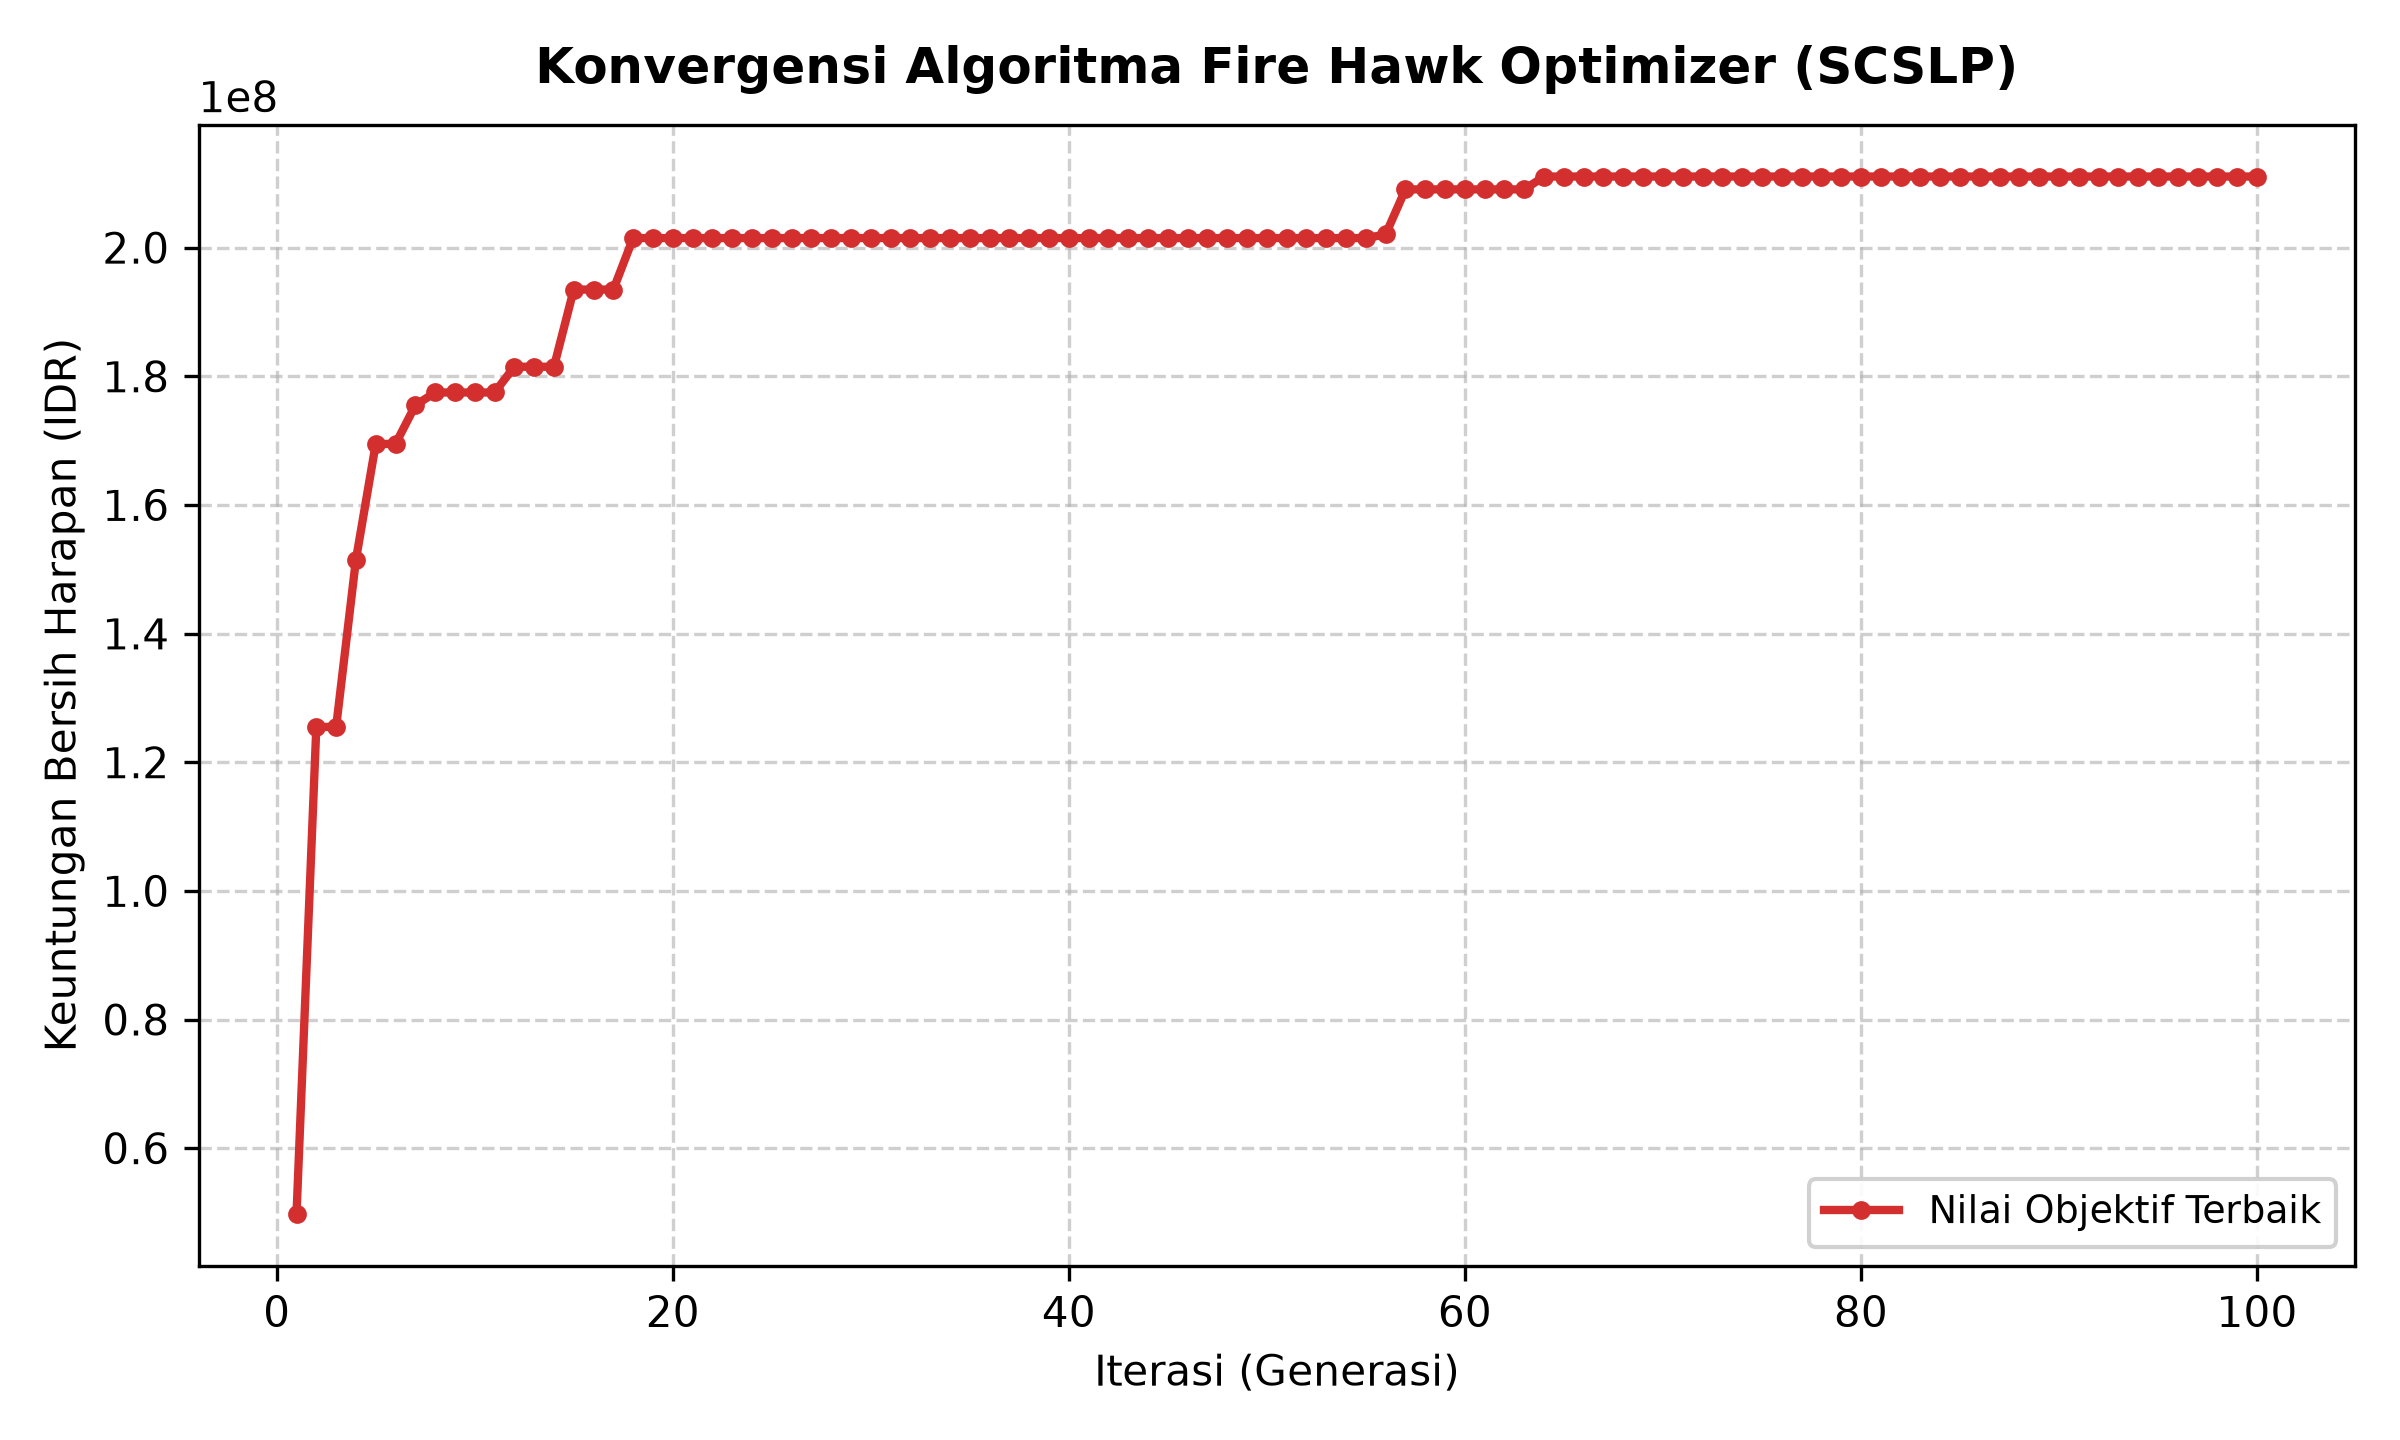
\includegraphics[scale=0.45]{__results___0_1.png}
    \caption{Iterasi Algoritma \textit{Fire Hawk Optimizer}}
    \label{Iterasi Algoritma Fire Hawk Optimizer}
\end{figure}
Algoritma \textit{Fire Hawk Optimizer} melakukan proses iterasi untuk terus memperbaiki solusi seperti yang terlihat pada Gambar \ref{Iterasi Algoritma Fire Hawk Optimizer}. Pada setiap iterasi:
\begin{enumerate}
    \item posisi elang api dan mangsa diperbarui menggunakan persamaan yang telah didefinisikan sebelumnya,
    \item nilai fungsi objektif dari setiap solusi baru dievaluasi,
    \item solusi terbaik global ($GB$) diperbarui jika ditemukan solusi yang lebih baik, dan
    \item proses penentuan teritori, pembaruan posisi elang api, dan pembaruan posisi mangsa diulangi.
\end{enumerate}
Iterasi akan terus berlanjut hingga salah satu kriteria penghentian terpenuhi. Kriteria penghentian dapat berupa (\mycite{talbi2009metaheuristics}):
\begin{enumerate}
    \item mencapai jumlah iterasi maksimum yang telah ditentukan sebelumnya,
    \item mencapai batas waktu komputasi yang telah ditetapkan, dan
    \item mencapai tingkat konvergensi tertentu, dimana perbaikan solusi antar iterasi menjadi sangat kecil atau tidak signifikan.
\end{enumerate}
Setelah kriteria penghentian terpenuhi, algoritma akan berhenti dan mengembalikan solusi terbaik yang ditemukan sebagai konfigurasi optimal untuk sistem \textit{electric bike-sharing}. Solusi ini mencakup lokasi stasiun pengisian daya yang harus dibangun, alokasi sepeda listrik yang optimal, dan trip yang harus diterima.

\subsection{Output Simulasi}

Simulasi dilakukan dengan menggunakan \textit{Python}  dan diperoleh solusi optimal dengan menggunakan algoritma \textit{Fire Hawk Optimizer}. Gambar \ref{Peta stasiun yang dibangun dan trip yang diterima} menunjukkan lokasi stasiun yang dibuka dan trip yang diterima, dijelaskan juga hasil dari output, termasuk nilai untuk setiap variabel dan hasil fungsi objektif.

\begin{figure}[H]
    \centering
    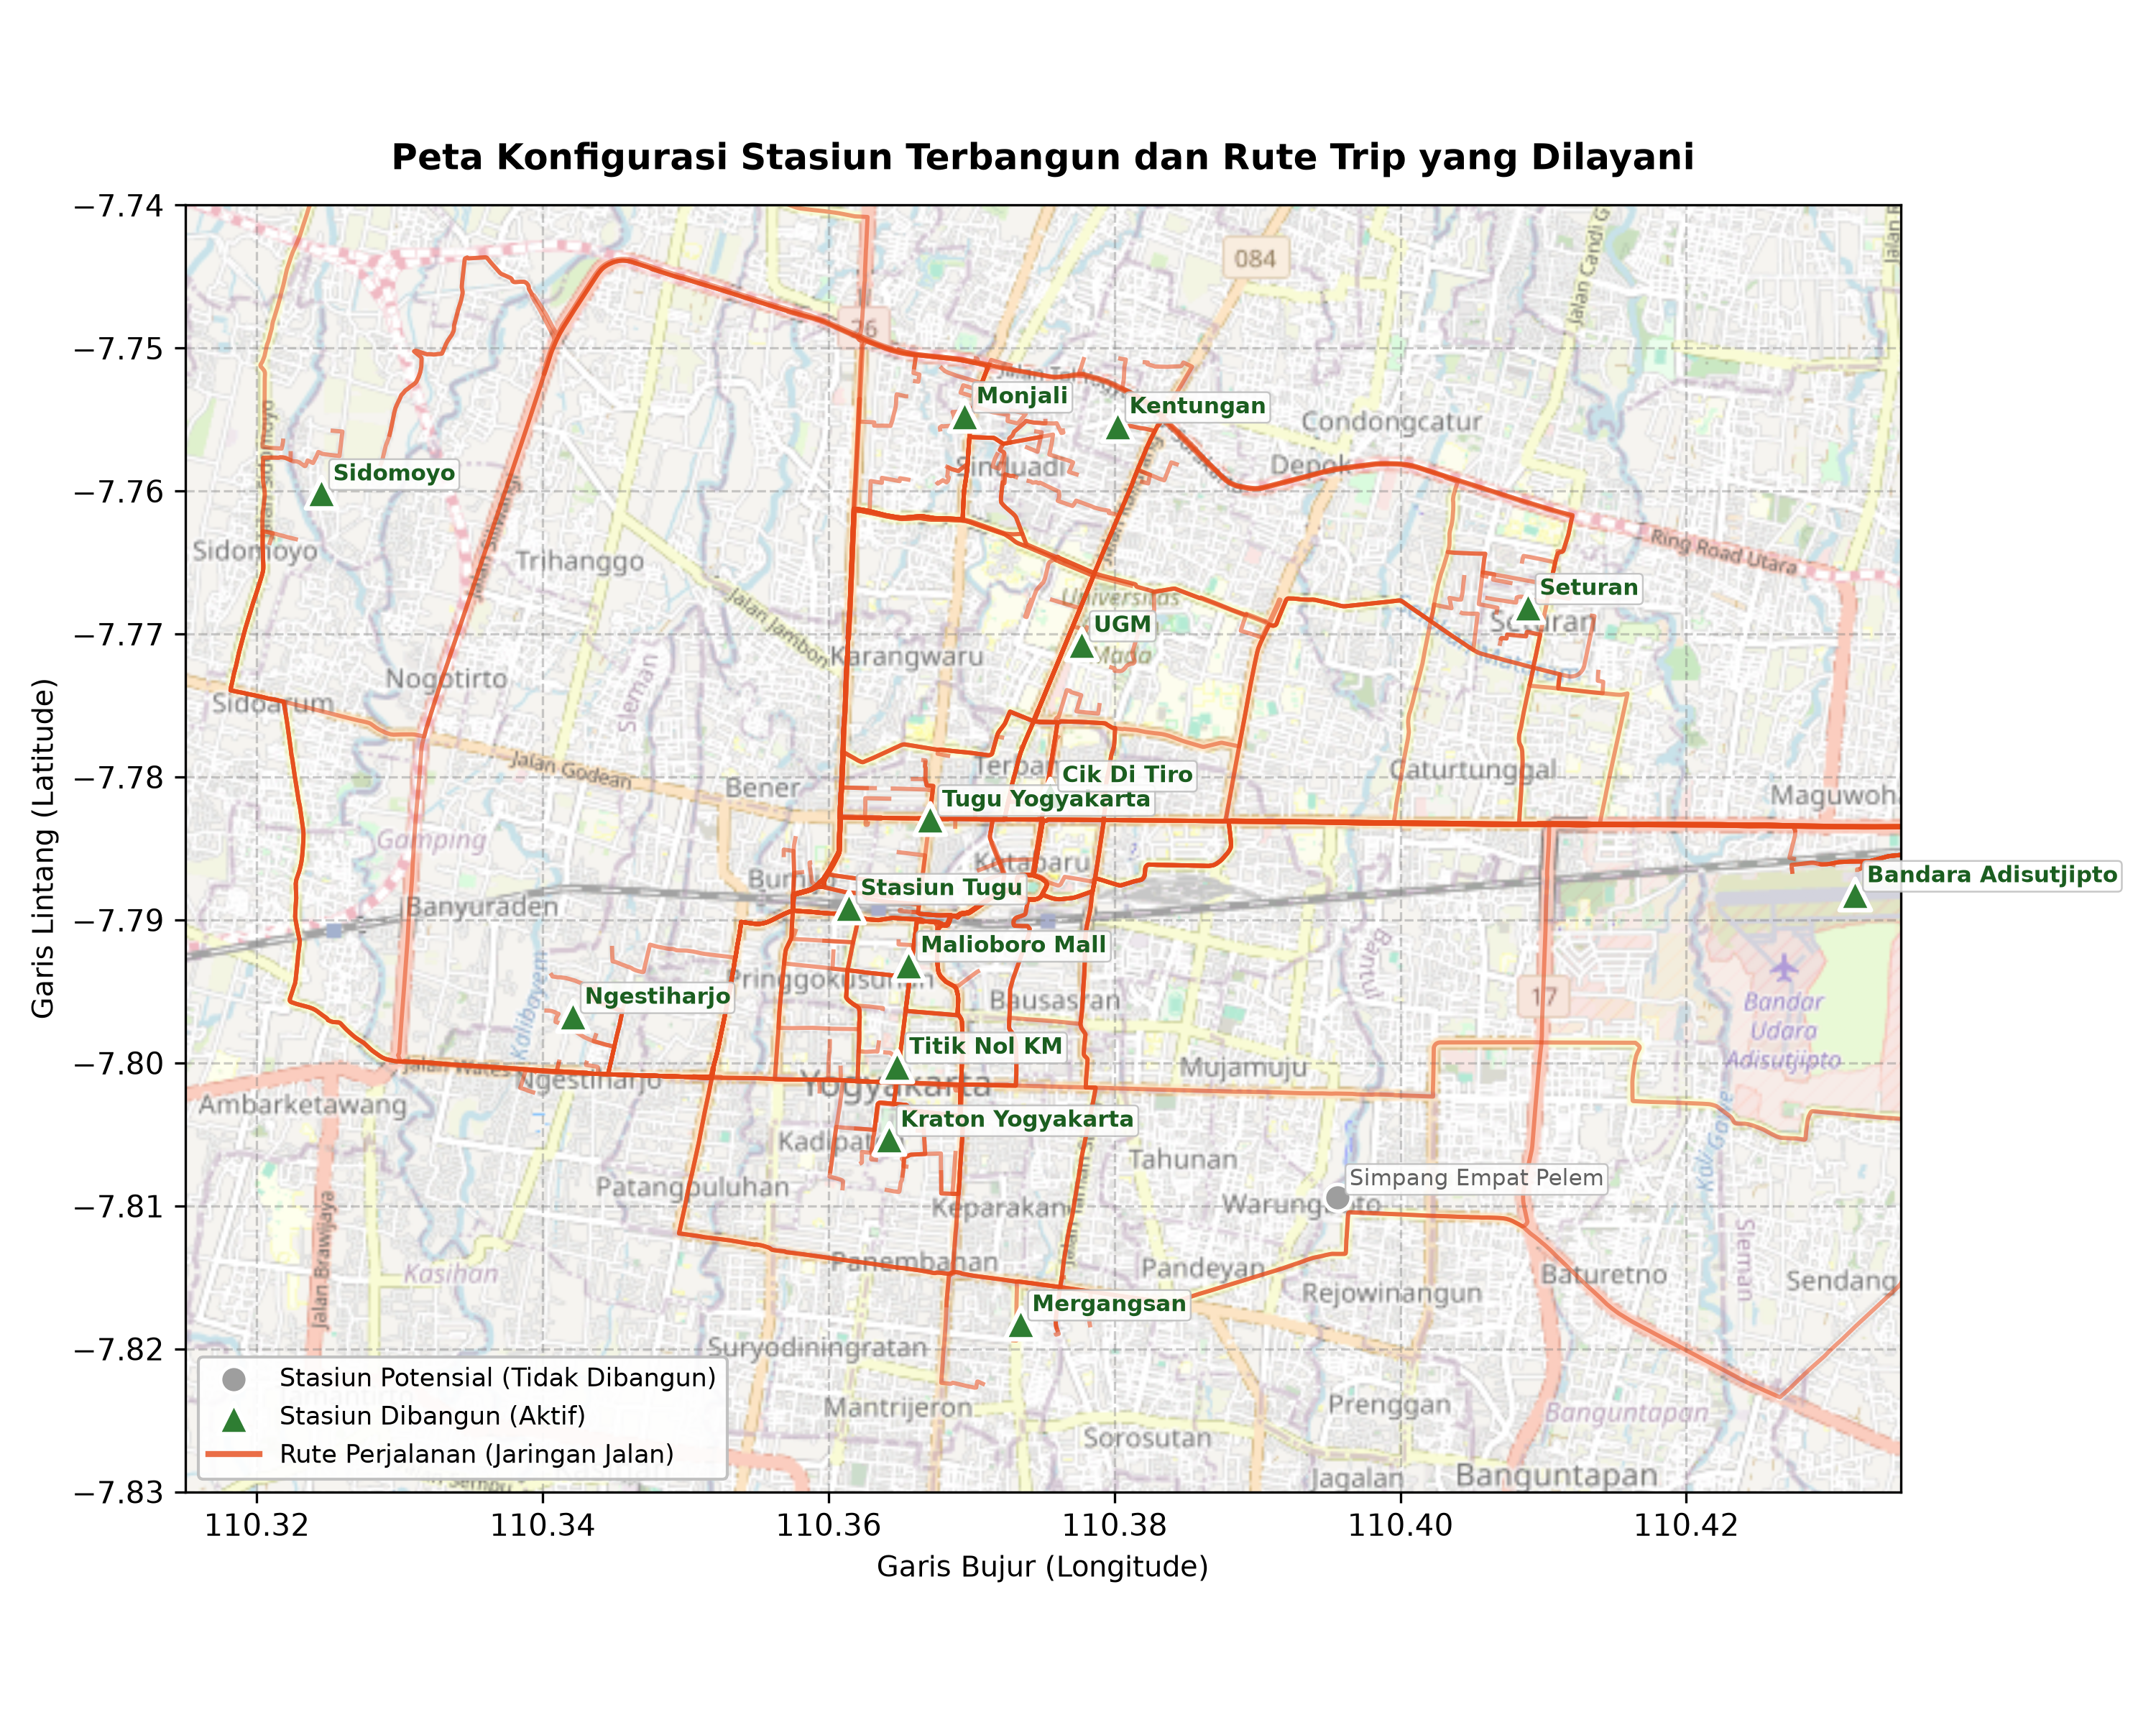
\includegraphics[scale=0.8]{hasil.png}
    \caption{Peta Stasiun yang Dibangun dan Trip yang Diterima}
    \label{Peta stasiun yang dibangun dan trip yang diterima}
\end{figure}

\subsubsection*{Variabel dan Hasil}
\begin{enumerate}
\item \textbf{Stasiun yang Dibangun (\(y\))}\\
Solusi optimal menunjukkan bahwa dari 15 lokasi potensial, 12 stasiun dipilih untuk dibangun, yaitu stasiun [1, 2, 3, 6, 7, 8, 9, 10, 11, 12, 13, 14]. Lokasi-lokasi ini meliputi (tidak dalam urutan).
\begin{enumerate}
\item Sidomoyo,
\item Monjali,
\item Kentungan,
\item Seturan,
\item Tugu,
\item Cik di Tiro,
\item Malioboro,
\item Simpang Empat Pelem,
\item Ngastiharjo,
\item Mergangsan,
\item Rejowinangun, dan
\item Bandara Adisucipto.
\end{enumerate}
Hal ini menandakan bahwa 80\% dari lokasi potensial dianggap strategis untuk mendukung operasi sistem \textit{bike-sharing}. Pemilihan lokasi ini mencakup berbagai area penting di Yogyakarta, termasuk pusat kota, area wisata, kawasan pendidikan, area bisnis dan pemukiman, serta titik-titik transportasi penting. 
\item \textbf{Sepeda yang Dibeli (\(b\))}\\
Model merekomendasikan pembelian 55 sepeda listrik. Jumlah ini mewakili keseimbangan optimal antara memenuhi permintaan yang diperkirakan dan mengelola biaya inventaris. Berikut lokasi terakhir sepeda listrik dari seluruh skenario.\\

\begin{tabular}{llcl}\hspace{-0.3em}
    (a) & \hspace{-0.5em}Sidomoyo &: & 8 sepeda, \\
    (b) & \hspace{-0.5em}Monjali &: & 1 sepeda,\\
    (c) & \hspace{-0.5em}Kentungan &: & 2 sepeda,\\
    (d) & \hspace{-0.5em}Seturan &: & 7 sepeda,\\
    (e) & \hspace{-0.5em}Tugu &: & 4  sepeda,\\
    (f) & \hspace{-0.5em}Cik di Tiro &: & 5 sepeda,\\
    (g) & \hspace{-0.5em}Malioboro &: & 7 sepeda,\\
    (h) & \hspace{-0.5em}Simpang Empat Pelem &: & 5 sepeda,\\
    (i) & \hspace{-0.5em}Ngastiharjo &: & 3 sepeda,\\
    (j) & \hspace{-0.5em}Mergangsan &: & 8 sepeda,\\
    (k) & \hspace{-0.5em}Rejowinangun &: & 7 sepeda, dan\\
    (l) & \hspace{-0.5em}Bandara Adisucipto &: & 4 sepeda.\\
\end{tabular}
\item \textbf{Trip yang Diterima (\(x\))}\\
Tingkat penerimaan trip bervariasi di antara skenario:
\begin{enumerate}
    \item Skenario 0 (Weekdays): 25/30 trip diterima (83.33\%)
    \item Skenario 1 (Saturday): 28/30 trip diterima (93.33\%)
    \item Skenario 2 (Sunday): 27/30 trip diterima (90.00\%)
\end{enumerate}
Tingkat penerimaan yang tinggi ini menunjukkan bahwa sistem yang diusulkan mampu memenuhi sebagian besar permintaan yang diproyeksikan, dengan kinerja terbaik pada hari Sabtu.
\end{enumerate}

Secara keseluruhan, solusi ini menunjukkan desain sistem \textit{bike-sharing} yang efisien terhadap permintaan dengan potensi keuntungan yang signifikan. Namun, masih ada ruang untuk penyempurnaan lebih lanjut, terutama dalam hal peningkatan utilisasi sepeda dan posibilitas optimasi lebih lanjut dari lokasi stasiun.
\chapter{PENUTUP}

Pada bab terakhir ini dituliskan kesimpulan dan saran-saran yang dapat diambil berdasarkan materi-materi yang telah dibahas pada bab-bab sebelumnya.

\section{Kesimpulan}
Berdasarkan pembahasan yang telah dilakukan sebelumnya, penulis menarik beberapa kesimpulan berikut:
\begin{enumerate}
    \item Masalah \textit{electric bike-sharing system} dapat dimodelkan dengan masalah stokastik dua tahap.
    \item Permasalahan-permasalahan optimisasi seperti \textit{electric bike-sharing system} dapat diselesaikan dengan algoritma \textit{metaheuristic} yang salah satunya yaitu \textit{Fire Hawk Optimizer}. Simulasi \textit{electric bike-sharing system} di kota Yogyakarta dengan parameter-parameter yang telah dipaparkan sebelumnya memberikan gambaran bahwa \textit{electric bike-sharing system} ini dapat terealisasi dengan nilai keuntungan sebesar 274.030.876 dengan stasiun-stasiun yang dibangun yaitu, Sidomoyo, Monjali, Kentungan, Seturan, Tugu, Cik di Tiro, Malioboro, Simpang Empat Pelem, Ngastiharjo, Mergangsan, Rejowinangun, Bandara Adisucipto serta 55 sepeda listrik yang dibeli dan 80 trip yang diterima.
\end{enumerate}

\section{Saran}
Formulasi \textit{two-stage stochastic} pada permasalahan \textit{electric bike-sharing system} dan penyelesaiannya dengan menggunakan algoritma \textit{Fire Hawk Optimizer} serta beberapa kesimpulan yang telah dituliskan di atas,  penulis ingin menyampaikan beberapa saran sebagai berikut.
\begin{enumerate}
    \item Penelitian selanjutnya dapat dikembangkan dengan membuat formulasi yang lebih efisien sehingga proses komputasi tidak memakan daya ataupun waktu yang lama.
    \item Perlu dilakukan penelitian lebih lanjut terutama \textit{benchmarking} metode penyelesaian permasalahan \textit{electric bike-sharing system} seperti dengan algoritma \textit{metaheuristic} lain misal \textit{particle swarm optimization, simulated annealing}, algoritma genetika, ataupun yang lain.
\end{enumerate}

%-----------------------------------------------------------------
%Disini akhir masukan Bab
%-----------------------------------------------------------------

%-----------------------------------------------------------------
%Disini awal masukan untuk Daftar Pustaka (ISI SESUAI DENGAN DATA ANDA!)
%-----------------------------------------------------------------
\begin{thebibliography}{99}
\addcontentsline{toc}{chapter}{DAFTAR PUSTAKA}

\bibitem[Azizi dkk.(2023)]{azizi2023fire}
Azizi, M. and Talatahari, S. and Gandomi, A. H., 2023, Fire Hawk Optimizer: a novel metaheuristic algorithm, \emph{Artificial Intelligence Review}, 56(1), 287--363.

\bibitem[Bikeplus(2016)]{bikeplus2016shared} 
Bikeplus, 2016. \emph{Shared Electric Bike Programme Report}. Carplus Trust, n.p..

\bibitem[Billingsley(1995)]{billingsley1995probability}
Billingsley, P., 1995, \emph{Probability and Measure}, 3rd ed., John Wiley \& Sons, New York.

\bibitem[Birge dan Louveaux(2011)]{birge2011introduction}
Birge, J. R., Louveaux, F., 2011, \emph{Introduction to stochastic programming}, Springer Science \& Business Media, London.

\bibitem[Boyd dan Vandenberghe(2004)]{boyd2004convex}
Boyd, S., Vandenberghe, L., 2004, \emph{Convex optimization}, Cambridge University Press, Cambridge.

\bibitem[BPS(2020)]{bps2020yogyakarta}
BPS, 2020, \emph{Statistik Kepariwisataan Daerah Istimewa Yogyakarta 2019}, Badan Pusat Statistik Provinsi D.I. Yogyakarta.

\bibitem[Brandstätter dkk.(2017)]{brandstatter2017determining}
Brandstätter, G. and Kahr, M. and Leitner, M., 2017, Determining optimal locations for charging stations of electric car-sharing systems under stochastic demand, \emph{Transportation Research Part B: Methodological}, 104, 17--35.

\bibitem[Campbell dkk.(2016)]{campbell2016electric} 
Campbell, A. A., Cherry, C. R., Ryerson, M. S., Yang, X., 2016. Factors influencing the choice of shared bicycles and shared electric bikes in Beijing. \emph{Transportation Research Part C: Emerging Technologies}, 67, 399-414.

\bibitem[Casella dan Berger(2002)]{casella2002statistical}
Casella, G. and Berger, R. L., 2002, \emph{Statistical Inference}, Duxbury.

\bibitem[Chen dkk.(2020)]{chen2020electric}
Chen, T. D. and Kockelman, K. M. and Khan, M., 2020, The electric vehicle charging station location problem: A parking-based assignment method for Seattle, \emph{Transportation Research Part D: Transport and Environment}, 78, 102132.

\bibitem[Fishman(2020)]{fishman2020bikeshare}
Fishman, E., 2020, Bikeshare: A Review of Recent Literature, \emph{Transport Reviews}, 40(6), 744--767.

\bibitem[Fyhri dan Fearnley(2017)]{fyhri2017effect} 
Fyhri, A., Fearnley, N., 2017. Effects of e-bikes on bicycle use and mode share. \emph{Transportation Research Part D: Transport and Environment}, 36, 45-52.

\bibitem[Glover(1986)]{glover1986future} 
Glover, F., 1986. \emph{Future paths for integer programming and links to artificial intelligence}. Computers \& operations research, 13(5), 533-549.

\bibitem[Grimmett dan Stirzaker(2020)]{grimmett2020probability}
Grimmett, G. and Stirzaker, D., 2020, \emph{Probability and Random Processes}, Oxford University Press, New York.

\bibitem[Haight(1967)]{haight1967handbook}
Haight, F. A., 1967, \emph{Handbook of the Poisson Distribution}, John Wiley \& Sons, New York.

\bibitem[Hastie dkk.(2009)]{hastie2009elements}
Hastie, T. and Tibshirani, R. and Friedman, J., 2009, \emph{The elements of statistical learning: data mining, inference, and prediction}, Springer Science \& Business Media, New York.

\bibitem[Holland(1992)]{holland1992adaptation}
Holland, J. H., 1992, \emph{Adaptation in natural and artificial systems: an introductory analysis with applications to biology, control, and artificial intelligence}, MIT Press, Cambridge, MA.

\bibitem[Hunter(2007)]{hunter2007matplotlib}
Hunter, J. D., 2007, Matplotlib: A 2D graphics environment, \emph{Computing in Science \& Engineering}, 9(3), 90--95.

\bibitem[IEA(2021)]{iea2021global}
IEA, 2021, \emph{Global EV Outlook 2021}, International Energy Agency, Paris.

\bibitem[Langford dkk.(2013)]{langford2013comparing} 
Langford, B. C., Cherry, C. R., Bassett Jr, D. R., Fitzhugh, E. C., Dhakal, N., 2013. Comparing physical activity of pedal-assist electric bikes with walking and conventional bicycles. \emph{Journal of Transport \& Health}, 4(1), 86-93.

\bibitem[Ling dkk.(2017)]{ling2017emerging} 
Ling, Z., Cherry, C. R., Yang, H., Jones, L. R., 2017. From e-bike to car: A study on factors influencing motorization of e-bike users across China. \emph{Transportation Research Part D: Transport and Environment}, 41, 50-63.

\bibitem[Ma dkk.(2020)]{ma2020electric} 
Ma, X., Yuan, Y., Van Oort, N., Hoogendoorn, S., 2020. Bike-sharing systems' impact on modal shift: A case study in Delft, the Netherlands. \emph{Journal of Cleaner Production}, 259, 120846.

\bibitem[MacMichael(2021)]{roadcc2021}
MacMichael, S., 2021, Plan for compulsory e-bike insurance in Spain faces fierce opposition, \emph{road.cc}, \url{https://road.cc/content/news/mandatory-bike-insurance-spain-291997} (diakses pada 20 September 2024).

\bibitem[McKinney(2011)]{mckinney2011pandas}
McKinney, W., 2011, pandas: a foundational Python library for data analysis and statistics, \emph{Python for High Performance and Scientific Computing}, 14(9), 1--9.

\bibitem[Nocedal dan Wright(2006)]{nocedal2006numerical} 
Nocedal, J., Wright, S., 2006. \emph{Numerical optimization}. Springer Science \& Business Media, New York, NY.

\bibitem[O'Brien dkk.(2014)]{obrien2014mining}
O'Brien, O. and Cheshire, J. and Batty, M., 2014, Mining bicycle sharing data for generating insights into sustainable transport systems, \emph{Journal of Transport Geography}, 34, 262--273.

\bibitem[Pemkot Yogyakarta(2020)]{pemkot2020yogyakarta}
Pemkot Yogyakarta, 2020, \emph{Rencana Pembangunan Jangka Menengah Daerah Kota Yogyakarta 2017-2022}, Pemerintah Kota Yogyakarta.

\bibitem[Powell(2019)]{powell2019unified}
Powell, W. B., 2019, A unified framework for stochastic optimization, \emph{European Journal of Operational Research}, 275(3), 795--821.

\bibitem[Ross(1996)]{ross1996stochastic}
Ross, S. M., 1996, \emph{Stochastic Processes}, John Wiley \& Sons, New York.

\bibitem[Ross(2014)]{ross2014introduction}
Ross, S. M., 2014, \emph{Introduction to Probability Models}, Academic Press, Burlington, MA.

\bibitem[Shaheen et al.(2019)]{shaheen2019sharing}
Shaheen, S., Cohen, A., Chan, N., Bansal, A., 2019, Sharing strategies: carsharing, shared micromobility (bikesharing and scooter sharing), transportation network companies, microtransit, and other innovative mobility modes, \emph{Transportation, Land Use, and Environmental Planning}, 237--262.

\bibitem[Sun dkk.(2018)]{sun2018data} 
Sun, Y., Mobasheri, A., Hu, X., Wang, W., 2018. Investigating impacts of environmental factors on the cycling behavior of bicycle-sharing users. \emph{Sustainability}, 9(6), 1060.

\bibitem[Talbi(2009)]{talbi2009metaheuristics}
Talbi, E. G., 2009, Metaheuristics: from design to implementation, \emph{John Wiley \& Sons}, Hoboken, NJ, 37--39.

\bibitem[UNFCCC(2015)]{unfccc2015paris}
UNFCCC, 2015, \emph{Paris Agreement}, United Nations, Paris.

\bibitem[UN(2015)]{un2015transforming}
United Nations General Assembly, 2015, Transforming our world: The 2030 agenda for sustainable development, \emph{United Nations General Assembly}, A/RES/70/1. Available at: \url{https://sustainabledevelopment.un.org/post2015/transformingourworld}.

\bibitem[Wilson(1996)]{wilson1996introduction}
Wilson, R. J., 1996, \emph{Introduction to Graph Theory}, Longman, Harlow.

\bibitem[Winston dan Goldberg(2004)]{winston2004operations}
Winston, W. L. and Goldberg, J. B., 2004, \emph{Operations research: applications and algorithms}, Vol. 3, Thomson Brooks/Cole, Belmont.

\bibitem[Zhu dkk.(2016)]{zhu2016charging}
Zhu, L. and Gonder, J. and Lin, Z., 2016, Charging station location problem of plug-in electric vehicles, \emph{Journal of Transport Geography}, 52, 11--22.

\end{thebibliography}
%-----------------------------------------------------------------
%-----------------------------------------------------------------


%-----------------------------------------------------------------
%Disini awal masukan untuk Lampiran (JIKA DIPERLUKAN)
%-----------------------------------------------------------------
\appendix

\chapter{DATA}

\begin{table}[H]
\centering
\caption{Data Stasiun}
\label{Station Data}
\begin{tabular}{|c|c|c|c|c|}
\hline
\textbf{station\_id} & \textbf{capacity} & \textbf{opening\_cost} & \textbf{latitude} & \textbf{longitude} \\
\hline
0 & 8 & 64475368 & -7.7891 & 110.3614 \\
1 & 7 & 29062142 & -7.7931 & 110.3656 \\
2 & 8 & 53604018 & -7.7824 & 110.3750 \\
3 & 5 & 54169124 & -7.7830 & 110.3657 \\
4 & 5 & 70770109 & -7.7801 & 110.3712 \\
5 & 9 & 79681206 & -7.7764 & 110.3632 \\
6 & 6 & 68409814 & -7.816507590225311 & 110.37882377262206 \\
7 & 9 & 58627082 & -7.764545623765107 & 110.36998599777583 \\
8 & 9 & 87155237 & -7.758517422697779 & 110.38959483165141 \\
9 & 10 & 56627802 & -7.804273754947625 & 110.4149690263108 \\
10 & 5 & 64476799 & -7.758885258655926 & 110.32442053616289 \\
11 & 9 & 55915390 & -7.7667612206468375 & 110.41185548735434 \\
12 & 10 & 64731553 & -7.810665575510653 & 110.39030027249711 \\
13 & 5 & 57354989 & -7.797234234968725 & 110.32582055624444 \\
14 & 7 & 52547174 & -7.815663727363731 & 110.34298468522442 \\
\hline
\end{tabular}
\end{table}

\begin{table}[H]
\centering
\caption{Weekday Data Skenario dan Profit}
\label{Weekday Data Skenario dan Profit}
\begin{tabular}{|c|c|c|c|}
\hline
\textbf{Scenario} & \textbf{Trip ID} & \textbf{Destination} & \textbf{Profit} \\
\hline

Weekdays & 0 & (-7.792931179673451, 110.36593183784399) & 30000000 \\
Weekdays & 1 & (-7.775647815981623, 110.36724251595128) & 20000000 \\
Weekdays & 2 & (-7.800520210506863, 110.41480096138257) & 20000000 \\
Weekdays & 3 & (-7.769890027550567, 110.41249566091625) & 20000000 \\
Weekdays & 4 & (-7.812769098888491, 110.39224477396209) & 20000000 \\
Weekdays & 5 & (-7.776569094401348, 110.37288896664307) & 30000000 \\
Weekdays & 6 & (-7.805526526949287, 110.41676671215377) & 10000000 \\
Weekdays & 7 & (-7.770438134482901, 110.36159240469725) & 30000000 \\
Weekdays & 8 & (-7.805665405269387, 110.41645859073208) & 20000000 \\
Weekdays & 9 & (-7.805541747688057, 110.38990179513809) & 10000000 \\
Weekdays & 10 & (-7.761427938777749, 110.32886417224998) & 30000000 \\
Weekdays & 11 & (-7.800388527425106, 110.32471770304838) & 20000000 \\
Weekdays & 12 & (-7.801710289960986, 110.32659754105705) & 30000000 \\
Weekdays & 13 & (-7.800040916629955, 110.41611241279443) & 20000000 \\
Weekdays & 14 & (-7.754633697351422, 110.32873446979093) & 30000000 \\
Weekdays & 15 & (-7.796324586945069, 110.36600172032915) & 20000000 \\
Weekdays & 16 & (-7.763738531763849, 110.32534399418394) & 30000000 \\
Weekdays & 17 & (-7.771354263023364, 110.41488578879236) & 30000000 \\
Weekdays & 18 & (-7.803140288211153, 110.32618939992823) & 10000000 \\
Weekdays & 19 & (-7.764528569476906, 110.3198398775548) & 30000000 \\
Weekdays & 20 & (-7.793381694707156, 110.36545130279752) & 30000000 \\
Weekdays & 21 & (-7.783222844979383, 110.37109768424821) & 30000000 \\
Weekdays & 22 & (-7.814171214257905, 110.38299766811353) & 20000000 \\
Weekdays & 23 & (-7.805631999110501, 110.39071673422443) & 30000000 \\
Weekdays & 24 & (-7.785064224320225, 110.36569285174483) & 10000000 \\
Weekdays & 25 & (-7.820291802236042, 110.38370114302596) & 10000000 \\
Weekdays & 26 & (-7.788425603038559, 110.3618555932266) & 10000000 \\
Weekdays & 27 & (-7.781567806650796, 110.36698710627229) & 30000000 \\
Weekdays & 28 & (-7.760737076884888, 110.32272475287424) & 30000000 \\
Weekdays & 29 & (-7.76346096101143, 110.39499553264821) & 10000000 \\

\hline
\end{tabular}
\end{table}
\begin{table}[H]
\centering
\caption{Saturday Data Skenario dan Profit}
\label{Saturday Data Skenario dan Profit}
\begin{tabular}{|c|c|c|c|}
\hline
\textbf{Scenario} & \textbf{Trip ID} & \textbf{Destination} & \textbf{Profit} \\
\hline

Saturday & 0 & (-7.75871107773189, 110.39134815553926) & 20000000 \\
Saturday & 1 & (-7.818683948045408, 110.38043422876682) & 10000000 \\
Saturday & 2 & (-7.819162310093343, 110.37643519677164) & 10000000 \\
Saturday & 3 & (-7.793072124436985, 110.36907039943321) & 10000000 \\
Saturday & 4 & (-7.815685814372376, 110.34690484321186) & 30000000 \\
Saturday & 5 & (-7.786874516259785, 110.36954395081311) & 30000000 \\
Saturday & 6 & (-7.779588526556111, 110.37001583609423) & 30000000 \\
Saturday & 7 & (-7.814312023834777, 110.39423259841826) & 10000000 \\
Saturday & 8 & (-7.786823838943322, 110.36906116005858) & 30000000 \\
Saturday & 9 & (-7.795136348660938, 110.33049748925366) & 10000000 \\
Saturday & 10 & (-7.753613497144761, 110.32635997594211) & 10000000 \\
Saturday & 11 & (-7.820813850628063, 110.3371846465614) & 20000000 \\
Saturday & 12 & (-7.7607050501917065, 110.32083135006967) & 30000000 \\
Saturday & 13 & (-7.794864016923349, 110.32354010961637) & 20000000 \\
Saturday & 14 & (-7.7811530039246355, 110.37023645423197) & 30000000 \\
Saturday & 15 & (-7.7792830658680945, 110.37132394967563) & 20000000 \\
Saturday & 16 & (-7.757683191947154, 110.32297643633814) & 30000000 \\
Saturday & 17 & (-7.78220799361297, 110.37915371308083) & 30000000 \\
Saturday & 18 & (-7.798025226732104, 110.32777940593454) & 10000000 \\
Saturday & 19 & (-7.817076175571514, 110.37979932423605) & 30000000 \\
Saturday & 20 & (-7.777854216274366, 110.37343442033261) & 10000000 \\
Saturday & 21 & (-7.791149772363954, 110.3702851624637) & 10000000 \\
Saturday & 22 & (-7.785429750117955, 110.36018833237053) & 30000000 \\
Saturday & 23 & (-7.787393884777669, 110.36406566304566) & 20000000 \\
Saturday & 24 & (-7.811308255015415, 110.34260012329163) & 30000000 \\
Saturday & 25 & (-7.813860746612476, 110.3918175913882) & 10000000 \\
Saturday & 26 & (-7.81301638041292, 110.34033159647704) & 30000000 \\
Saturday & 27 & (-7.767798790112538, 110.41504464936352) & 20000000 \\
Saturday & 28 & (-7.782394523032584, 110.3670622693528) & 10000000 \\
Saturday & 29 & (-7.7838892603336225, 110.37427530337268) & 30000000 \\

\hline
\end{tabular}
\end{table}
\begin{table}[H]
\centering
\caption{Sunday Data Skenario dan Profit}
\label{Sunday Data Skenario dan Profit}
\begin{tabular}{|c|c|c|c|}
\hline
\textbf{Scenario} & \textbf{Trip ID} & \textbf{Destination} & \textbf{Profit} \\
\hline

Sunday & 0 & (-7.754752211101029, 110.31954432750135) & 30000000 \\
Sunday & 1 & (-7.801083456349155, 110.41582559786396) & 10000000 \\
Sunday & 2 & (-7.786741537607359, 110.36497806889548) & 20000000 \\
Sunday & 3 & (-7.77526140556621, 110.36610537165039) & 10000000 \\
Sunday & 4 & (-7.79793487443431, 110.36460546575) & 10000000 \\
Sunday & 5 & (-7.779393206442219, 110.37283933382679) & 30000000 \\
Sunday & 6 & (-7.765079428939965, 110.40791648049658) & 30000000 \\
Sunday & 7 & (-7.766483431597694, 110.36441998748231) & 20000000 \\
Sunday & 8 & (-7.772728610153513, 110.4081503856958) & 10000000 \\
Sunday & 9 & (-7.786007661386255, 110.3632971806047) & 10000000 \\
Sunday & 10 & (-7.759109290071894, 110.3277243573456) & 10000000 \\
Sunday & 11 & (-7.762074840637407, 110.4150550488201) & 10000000 \\
Sunday & 12 & (-7.801513788859254, 110.32921371250177) & 10000000 \\
Sunday & 13 & (-7.805540404637923, 110.39088484416312) & 20000000 \\
Sunday & 14 & (-7.783618490223531, 110.36677941388547) & 10000000 \\
Sunday & 15 & (-7.77096639688936, 110.41728666003176) & 30000000 \\
Sunday & 16 & (-7.767945092577382, 110.3727601660306) & 30000000 \\
Sunday & 17 & (-7.781030790251795, 110.37113705794233) & 30000000 \\
Sunday & 18 & (-7.777079017004526, 110.3704256347233) & 30000000 \\
Sunday & 19 & (-7.783838142517056, 110.36690204433873) & 30000000 \\
Sunday & 20 & (-7.783720084159466, 110.36639890659504) & 20000000 \\
Sunday & 21 & (-7.767531353710349, 110.36535251914106) & 10000000 \\
Sunday & 22 & (-7.760215186126595, 110.38419678669128) & 20000000 \\
Sunday & 23 & (-7.8204016238634235, 110.37917718252952) & 30000000 \\
Sunday & 24 & (-7.783875491808733, 110.3759394151611) & 10000000 \\
Sunday & 25 & (-7.792707835752402, 110.32539392047775) & 10000000 \\
Sunday & 26 & (-7.798172099226585, 110.3650017074385) & 10000000 \\
Sunday & 27 & (-7.759285126664732, 110.31979258704025) & 10000000 \\
Sunday & 28 & (-7.791043820302062, 110.36105716198279) & 30000000 \\
Sunday & 29 & (-7.8035972514521195, 110.4128934623853) & 10000000 \\
\hline
\end{tabular}
\end{table}

\begin{table}[H]
\centering
\caption{Weekday Data Skenario Lainnya}
\label{Weekday Data Skenario Lainnya}
\begin{tabular}{|c|c|c|c|c|c|}
\hline
\textbf{Scenario} & \textbf{Trip ID} & \textbf{Start Time} & \textbf{End Time} & \textbf{Battery Consumption} & \textbf{Probability} \\
\hline
Weekdays & 0 & 5 & 8 & 0.062217669587698386 & 0.3 \\
Weekdays & 1 & 0 & 2 & 0.10701353654407111 & 0.3 \\
Weekdays & 2 & 0 & 2 & 0.11670451517626136 & 0.3 \\
Weekdays & 3 & 2 & 4 & 0.08936807656614155 & 0.3 \\
Weekdays & 4 & 6 & 8 & 0.20747699405596637 & 0.3 \\
Weekdays & 5 & 11 & 14 & 0.024080815488423665 & 0.3 \\
Weekdays & 6 & 2 & 3 & 0.10142192376549508 & 0.3 \\
Weekdays & 7 & 7 & 10 & 0.054632223929739564 & 0.3 \\
Weekdays & 8 & 7 & 9 & 0.12814905906809582 & 0.3 \\
Weekdays & 9 & 6 & 7 & 0.019610493595530708 & 0.3 \\
Weekdays & 10 & 9 & 12 & 0.2154004464729302 & 0.3 \\
Weekdays & 11 & 7 & 9 & 0.08832422022992438 & 0.3 \\
Weekdays & 12 & 5 & 8 & 0.19008947396952916 & 0.3 \\
Weekdays & 13 & 0 & 2 & 0.11255325564876342 & 0.3 \\
Weekdays & 14 & 6 & 9 & 0.0231471433421849 & 0.3 \\
Weekdays & 15 & 11 & 13 & 0.09379349819987594 & 0.3 \\
Weekdays & 16 & 2 & 5 & 0.17889024517920643 & 0.3 \\
Weekdays & 17 & 9 & 12 & 0.13330727442589083 & 0.3 \\
Weekdays & 18 & 11 & 12 & 0.014907193928993319 & 0.3 \\
Weekdays & 19 & 11 & 14 & 0.2132098621812017 & 0.3 \\
Weekdays & 20 & 4 & 7 & 0.03701767027148605 & 0.3 \\
Weekdays & 21 & 7 & 10 & 0.06093130705466953 & 0.3 \\
Weekdays & 22 & 4 & 6 & 0.07946732982412702 & 0.3 \\
Weekdays & 23 & 8 & 11 & 0.05693256159547741 & 0.3 \\
Weekdays & 24 & 5 & 6 & 0.08278664879613755 & 0.3 \\
Weekdays & 25 & 4 & 5 & 0.12421131504639817 & 0.3 \\
Weekdays & 26 & 1 & 2 & 0.010783588598240176 & 0.3 \\
Weekdays & 27 & 5 & 8 & 0.04084386509049799 & 0.3 \\
Weekdays & 28 & 1 & 4 & 0.11855108116108053 & 0.3 \\
Weekdays & 29 & 10 & 11 & 0.05977798087267876 & 0.3 \\
\hline
\end{tabular}
\end{table}
\begin{table}[H]
\centering
\caption{Saturday Data Skenario Lainnya}
\label{Saturday Data Skenario Lainnya}
\begin{tabular}{|c|c|c|c|c|c|}
\hline
\textbf{Scenario} & \textbf{Trip ID} & \textbf{Start Time} & \textbf{End Time} & \textbf{Battery Consumption} & \textbf{Probability} \\
\hline
Saturday & 0 & 1 & 3 & 0.0704929393661057 & 0.34 \\
Saturday & 1 & 11 & 12 & 0.1408308207340015 & 0.34 \\
Saturday & 2 & 4 & 5 & 0.07657157502211483 & 0.34 \\
Saturday & 3 & 4 & 5 & 0.0762383045030205 & 0.34 \\
Saturday & 4 & 7 & 10 & 0.12974420975932455 & 0.34 \\
Saturday & 5 & 8 & 11 & 0.0900320649903682 & 0.34 \\
Saturday & 6 & 3 & 6 & 0.014910720550740638 & 0.34 \\
Saturday & 7 & 11 & 12 & 0.10955778541781142 & 0.34 \\
Saturday & 8 & 11 & 14 & 0.019547159811202117 & 0.34 \\
Saturday & 9 & 10 & 11 & 0.0812661837131828 & 0.34 \\
Saturday & 10 & 9 & 10 & 0.18976945572060308 & 0.34 \\
Saturday & 11 & 7 & 9 & 0.20400287179010476 & 0.34 \\
Saturday & 12 & 8 & 11 & 0.11797275813721532 & 0.34 \\
Saturday & 13 & 2 & 4 & 0.04809157471702315 & 0.34 \\
Saturday & 14 & 1 & 4 & 0.10891074821327364 & 0.34 \\
Saturday & 15 & 10 & 12 & 0.023010295084486324 & 0.34 \\
Saturday & 16 & 7 & 10 & 0.10993672671294834 & 0.34 \\
Saturday & 17 & 10 & 13 & 0.0604823726783922 & 0.34 \\
Saturday & 18 & 1 & 2 & 0.18857674489125542 & 0.34 \\
Saturday & 19 & 1 & 4 & 0.06228447748438064 & 0.34 \\
Saturday & 20 & 4 & 5 & 0.050296854884397176 & 0.34 \\
Saturday & 21 & 11 & 12 & 0.11051186098286486 & 0.34 \\
Saturday & 22 & 0 & 3 & 0.017195518088264857 & 0.34 \\
Saturday & 23 & 9 & 11 & 0.023689490470052817 & 0.34 \\
Saturday & 24 & 0 & 3 & 0.11284957581239363 & 0.34 \\
Saturday & 25 & 8 & 9 & 0.08603452037998166 & 0.34 \\
Saturday & 26 & 5 & 8 & 0.010175224265666812 & 0.34 \\
Saturday & 27 & 6 & 8 & 0.055283163869471144 & 0.34 \\
Saturday & 28 & 9 & 10 & 0.002346555740345217 & 0.34 \\
Saturday & 29 & 10 & 13 & 0.13178957872592567 & 0.34 \\
\hline
\end{tabular}
\end{table}
\begin{table}[H]
\centering
\caption{Sunday Data Skenario Lainnya}
\label{Sunday Data Skenario Lainnya}
\begin{tabular}{|c|c|c|c|c|c|}
\hline
\textbf{Scenario} & \textbf{Trip ID} & \textbf{Start Time} & \textbf{End Time} & \textbf{Battery Consumption} & \textbf{Probability} \\
\hline
Sunday & 0 & 8 & 11 & 0.11069695699910045 & 0.36 \\
Sunday & 1 & 5 & 6 & 0.12681471196583274 & 0.36 \\
Sunday & 2 & 3 & 5 & 0.08151117212498699 & 0.36 \\
Sunday & 3 & 8 & 9 & 0.0950354466301667 & 0.36 \\
Sunday & 4 & 4 & 5 & 0.058674640322312115 & 0.36 \\
Sunday & 5 & 10 & 13 & 0.035824898097683106 & 0.36 \\
Sunday & 6 & 5 & 8 & 0.09061648088181894 & 0.36 \\
Sunday & 7 & 5 & 7 & 0.08849772530931686 & 0.36 \\
Sunday & 8 & 2 & 3 & 0.048885312447122145 & 0.36 \\
Sunday & 9 & 5 & 6 & 0.060853959747676746 & 0.36 \\
Sunday & 10 & 6 & 7 & 0.11042185401585164 & 0.36 \\
Sunday & 11 & 10 & 11 & 0.13271147208429795 & 0.36 \\
Sunday & 12 & 3 & 4 & 0.09772358246522068 & 0.36 \\
Sunday & 13 & 3 & 5 & 0.0452649216520342 & 0.36 \\
Sunday & 14 & 2 & 3 & 0.02348088579620471 & 0.36 \\
Sunday & 15 & 11 & 14 & 0.11782245056011577 & 0.36 \\
Sunday & 16 & 3 & 6 & 0.0038417288463018185 & 0.36 \\
Sunday & 17 & 8 & 11 & 0.02799553068716554 & 0.36 \\
Sunday & 18 & 1 & 4 & 0.02975269065720625 & 0.36 \\
Sunday & 19 & 4 & 7 & 0.10138149694701239 & 0.36 \\
Sunday & 20 & 7 & 9 & 0.009730430740964337 & 0.36 \\
Sunday & 21 & 8 & 9 & 0.03074333233255257 & 0.36 \\
Sunday & 22 & 3 & 5 & 0.05669477116352015 & 0.36 \\
Sunday & 23 & 10 & 13 & 0.12327249182452929 & 0.36 \\
Sunday & 24 & 1 & 2 & 0.029401556030399765 & 0.36 \\
Sunday & 25 & 8 & 9 & 0.012037544070469473 & 0.36 \\
Sunday & 26 & 10 & 11 & 0.07528869871973946 & 0.36 \\
Sunday & 27 & 3 & 4 & 0.018731418750935168 & 0.36 \\
Sunday & 28 & 5 & 8 & 0.01597100666376714 & 0.36 \\
Sunday & 29 & 7 & 8 & 0.20327934160326394 & 0.36 \\
\hline
\end{tabular}
\end{table}

\begin{table}[H]
\centering
\caption{Trip yang Diterima tiap Skenario}
\label{Accepted Trip IDs by Scenario}
\begin{tabular}{|c|c|c|}
\hline
\textbf{Hari Kerja} & \textbf{Sabtu} & \textbf{Minggu} \\
\hline
0 & 0 & 0 \\
1 & 2 & 1 \\
2 & 3 & 2 \\
3 & 4 & 4 \\
4 & 5 & 5 \\
5 & 6 & 6 \\
6 & 7 & 7 \\
7 & 8 & 8 \\
8 & 9 & 9 \\
9 & 10 & 10 \\
10 & 11 & 11 \\
11 & 12 & 12 \\
13 & 13 & 13 \\
14 & 14 & 14 \\
15 & 15 & 15 \\
16 & 16 & 16 \\
17 & 17 & 18 \\
18 & 18 & 19 \\
20 & 19 & 20 \\
21 & 20 & 21 \\
23 & 21 & 22 \\
24 & 22 & 23 \\
25 & 23 & 24 \\
27 & 24 & 25 \\
28 & 25 & 27 \\
 & 26 & 28 \\
 & 27 & 29 \\
 & 28 &  \\
\hline
\end{tabular}
\end{table}


\chapter{LAMPIRAN PENYELESAIAN SISTEM \textit{ELECTRIC BIKE-SHARING} SEDERHANA DENGAN LINGO}

\begin{verbatim}
MODEL:

! Objective function;
MAX = 0.70 * (Z11 + Z21) + 0.30 * (Z12 + Z22);

! Constraints;
X1 + X2 = 3;
X1 + W11 >= Z11;
X2 + W12 >= Z12;
W11 + W12 = 1;
Z11 <= 3;
Z12 <= 1;
X1 + W21 >= Z21;
X2 + W22 >= Z22;
W21 + W22 = 1;
Z21 <= 1;
Z22 <= 3;

! Non-negativity constraints;
@FREE(X1); @FREE(X2);
@BND(0, W11, 1); @BND(0, W12, 1);
@BND(0, W21, 1); @BND(0, W22, 1);
@BND(0, Z11, 3); @BND(0, Z12, 1);
@BND(0, Z21, 1); @BND(0, Z22, 3);

END
\end{verbatim}

\begin{figure}[H]
    \centering
    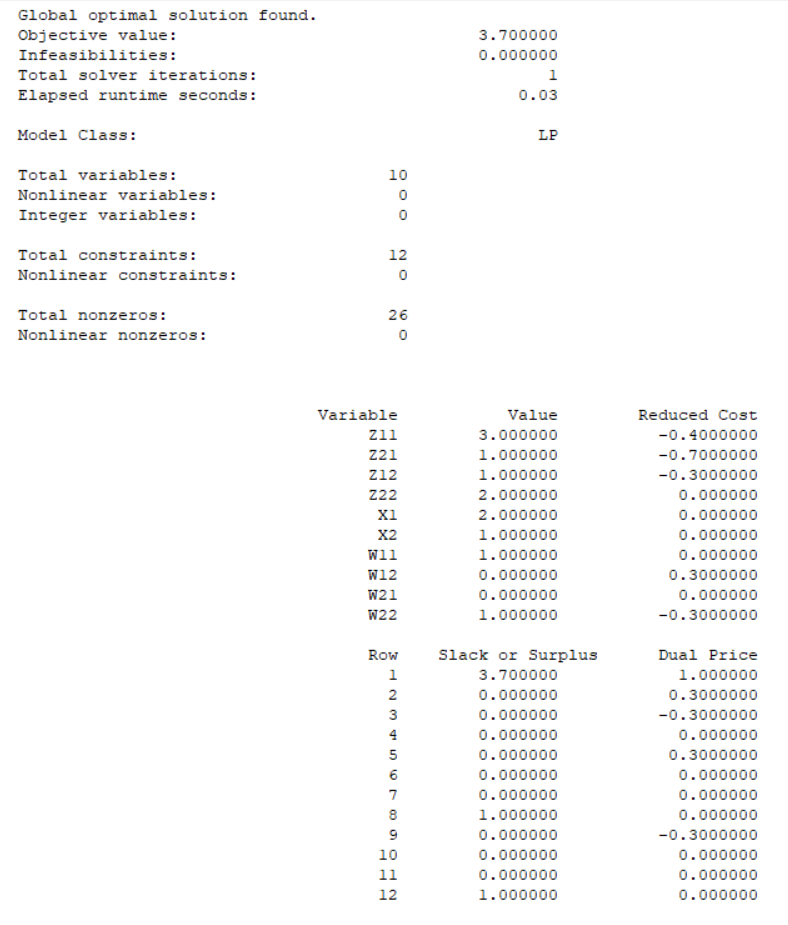
\includegraphics{LINGO.png}
    \caption{Hasil Model Sistem \textit{Electric Bike-Sharing} Sederhana}
    \label{LINGO}
\end{figure}

\chapter{LAMPIRAN SKRIP PROGRAM GENERATING DATA}
\lstset{language=python, frame=single}
\lstset{numbers=left, numberstyle=\tiny, stepnumber=1, numbersep=5pt, basicstyle=\footnotesize}
\lstset{xleftmargin=6pt, xrightmargin=8pt, rulesepcolor=\color{black}}
\lstset{keywordstyle=\color{blue},breaklines=true, breakindent=27pt}
\lstinputlisting{appendices/generator.py.txt}


\chapter{LAMPIRAN SKRIP PROGRAM PEMODELAN DAN KENDALA (SCSLP)}
\lstset{language=python, frame=single}
\lstset{numbers=left, numberstyle=\tiny, stepnumber=1, numbersep=5pt, basicstyle=\footnotesize}
\lstset{xleftmargin=6pt, xrightmargin=8pt, rulesepcolor=\color{black}}
\lstset{keywordstyle=\color{blue},breaklines=true, breakindent=27pt}
\lstinputlisting{appendices/problem.py.txt}

\chapter{LAMPIRAN SKRIP PENYELESAIAN ALGORITMA \textit{FIRE HAWK OPTIMIZER}}
\lstset{language=python, frame=single}
\lstset{numbers=left, numberstyle=\tiny, stepnumber=1, numbersep=5pt, basicstyle=\footnotesize}
\lstset{xleftmargin=6pt, xrightmargin=8pt, rulesepcolor=\color{black}}
\lstset{keywordstyle=\color{blue},breaklines=true, breakindent=27pt}
\lstinputlisting{appendices/fho.py.txt}

%-----------------------------------------------------------------
%-----------------------------------------------------------------
\end{document}
